%%%%% NXT_tutorial-1.0.7 %%%%%
%%%%%%%%%% PREAMBLE %%%%%%%%%%
\documentclass[11pt]{article}
\usepackage{amsmath}
\usepackage{graphicx}
\usepackage{wrapfig}
\usepackage{verbatim}
\usepackage{float}
\usepackage{makeidx}
\usepackage[top = 1in, bottom = 1in, right = 1in, left = 1in]{geometry}
\usepackage[pdftex]{hyperref}
\usepackage{program_article}
%%%%%%%%%% END of PREAMBLE %%%%%%%%%%
\title{Ch NXT Package User's Guide}
\author{Binsen Qian\\Mechanical and Aerospace Engeering}
\date{\today}
\makeindex
\begin{document}

%% Begin title page %%
\begin{titlepage}
\begin{center}
\vspace*{2cm}
{\Huge\sf\bf Ch NXT Package User's Guide}\\
\vspace*{2cm}
{\bf Version 1.0.7}\\
\vspace*{2cm}
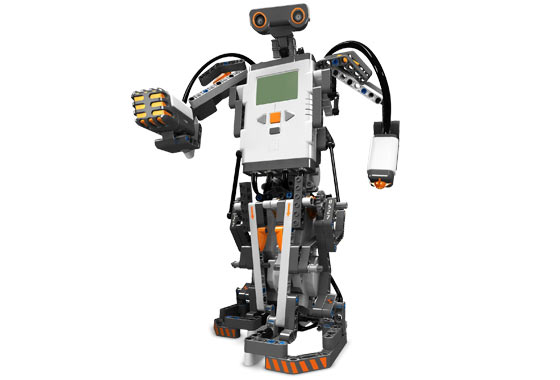
\includegraphics[width = 5in]{figure/mindstorm/NXT_humanoid.png}
\vspace*{2cm}
\newline
Integration Engineering Laboratory\\
University of California, Davis\\
Augest, 2012\\
\end{center}
\end{titlepage}
%% End title page %%

%% use roman page numbering %%
\pagenumbering{Roman}

%% Begin copyright %%
\newpage
\noindent
Copyright (c) 2012 Integration Engineering Laboratory\\
University of California, Davis \\
\newline
Permission to use and distribute this software and its
documentation for any purpose with or without fee is hereby granted,
provided that the above copyright notice appear in all copies and
that both that copyright notice and this permission notice appear
in supporting documentation.\\
\newline
This software is provided "as is" without express or implied warranty
to the extent permitted by applicable law.

%% End copyright %%

\newpage
\tableofcontents
\newpage

%% use arabic page numbering %%
\pagenumbering{arabic}
\baselineskip = 12 pt
%\vspace*{-1.5cm}\textbf{}

%%%%%%%%%%%%% Ch Mindstorms NXT Control Package %%%%%%%%%%%%
\section{Introduction}
Ch Mindstorms NXT Control Package brings the inherent functionality of the Ch programming language
to the intelligence and versatility found in the LEGO Mindstorms NXT robotic design system.\\

The Ch Mindstorms NXT Control Package consists of a set of API functions enabling programmers to 
write programs in C or C++ that can access and control the many features of the LEGO Mindstorms 
NXT controller. The API converts the complex messaging tasks required to communicate with the NXT 
into easy to use functions; allowing the user  to focus their efforts on their robotic application, 
rather than the details of communication. The API of the Ch Mindstorms NXT Control Package was 
designed to support and augment all of the functionality found in the LEGO Mindstorms NXT controller.
The Ch package further enhances the capabilities of the NXT controller by adding data collection and 
plotting capabilities. Additionally an NXT control program, written in C source code can be directly 
run from any platform in Ch without tedious compile/link/execute/debug cycles.\\

The communication between the user, the computer, the NXT controller, the sensors, and the motors can
be described in Figure \ref{fig_NXT_comm}. Once NXT is connected to the computer and a NXT program 
has started, the program instructions are sent from the computer to the NXT. The NXT controller will 
process these instructions perform appropriate tasks by sending commands to the motors or receiving 
data from the sensors. The NXT can collect sensor data and motor encoder counts, and the data can be 
sent back to the computer for further manipulation, display, or stored in the computer for the user.\\

%%%%% START OF FIGURE %%%%%
\begin{figure}[h]
  \begin{center}
    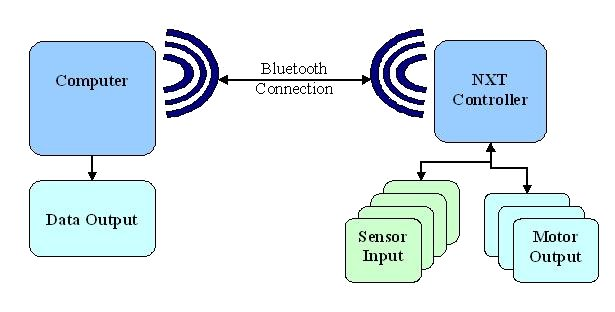
\includegraphics[height=2.5in]{figure/mindstorm/NXT_connect.png}
    \caption{Communication Diagram of NXT\label{fig_NXT_comm}}
  \end{center}
\end{figure}
%%%%% END OF FIGURE %%%%%

With Ch Mindstorms NXT Control Package, you can quickly develop an NXT robotic application and log 
your results. The ease of design and added functionality makes the Ch NXT Control Package a good 
candidate for any NXT programming application.\\

In this guide, we will go over the basics of a Ch Mindstorms NXT program. We will also discuss 
about how to control a NXT vehicle's motion. Lastly we will describe how to control non-vehicle
NXT robots. After reading this guide, you will be ready to write your own Ch NXT program to 
control your NXT robot.

\newpage
\section{Configuraing Lego Mindstorms NXT for Remote Control}
Before using the Ch NXT package to control NXTs, we need to configure the NXTs' bluetooth addresses.
Firstly, the NXT modules need to be paired with the PC, which tells the computer the device is able
to connect to. After successfully paired with the computer, we need to add the bluetooth addresses of
NXTs to the configuration files, which allows the \texttt{ChNXT API} \texttt{connect()} to access
those devices. The detailed information about paring part will be described in another documentation
and in the next part will introduce you how to setup the bluetooth addresses of NXTs to the Ch NXT
configuration file step by step.

\subsection{Getting Bluetooth Addresses of NXTs}
Firstly, we need to get the Bluetooth address of a NXT. As Figure~\ref{fig:bt_device} shown, right click
the Bluetooth icon in the right buttom corner.

%%%%% START OF FIGURE %%%%%
\begin{figure}[H]
  \begin{center}
    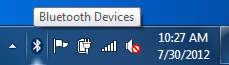
\includegraphics[height=0.5in]{figure/configuration/getBTaddress/bt1.png}
    \caption{Right click the Bluetooth icon.\label{fig:bt_device}}
  \end{center}
\end{figure}
%%%%% END OF FIGURE %%%%%

Then, choose the option "Show Bluetooth Devices", in Figure~\ref{fig:bt_show_device}, to find the NXT which 
has already paired with the computer.

%%%%% START OF FIGURE %%%%%
\begin{figure}[H]
  \begin{center}
    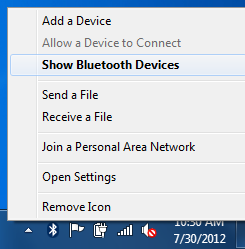
\includegraphics[height=3in]{figure/configuration/getBTaddress/btShowDevices.png}
    \caption{Choose "Show Bluetooth Devices" option.\label{fig:bt_show_device}}
  \end{center}
\end{figure}
%%%%% END OF FIGURE %%%%%

Then, a dialog with all paired Bluetooth devices in this dialog will appear on the screen. Find the NXT icon
and right click on the icon. Then choose "Properties" option as shown in Figure~\ref{fig:bt_property}.

%%%%% START OF FIGURE %%%%%
\begin{figure}[H]
  \begin{center}
    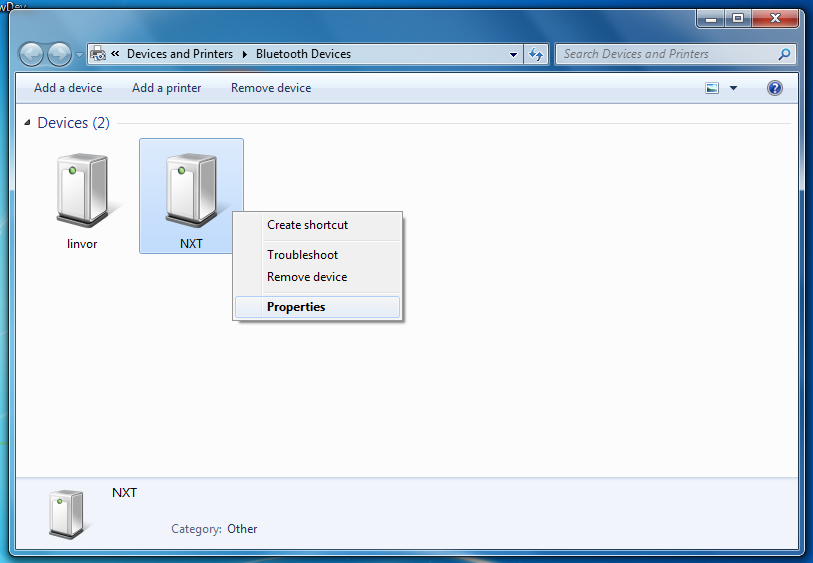
\includegraphics[height=3in]{figure/configuration/getBTaddress/btProperties.png}
    \caption{Right click the NXT icon then choose "Properties" option.\label{fig:bt_property}}
  \end{center}
\end{figure}
%%%%% END OF FIGURE %%%%%

In the dialog of NXT properties as shown in Figure~\ref{fig:bt_property_dialog}, click "Bluetooth" tab on the
top and the bluetooth address will show as "Unique identifier" with the format as "xx:xx:xx:xx:xx:xx".

%%%%% START OF FIGURE %%%%%
\begin{figure}[H]
  \begin{center}
    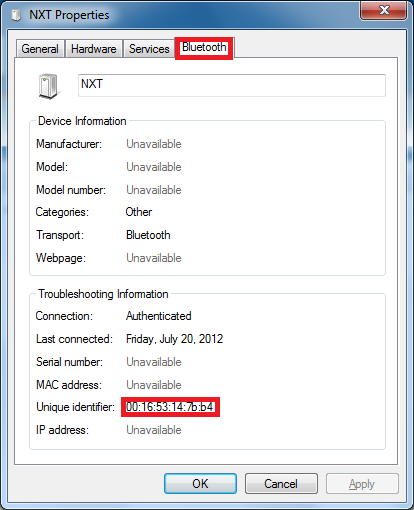
\includegraphics[height=3in]{figure/configuration/getBTaddress/btPropertiesDlg.png}
    \caption{The properties dialog.\label{fig:bt_property_dialog}}
  \end{center}
\end{figure}
%%%%% END OF FIGURE %%%%%

Now that we have already learned how to get the Bluetooth addresses of our NXTs, we can begin next section, which
will introduce you how to add the Bluetooth address we have gotten into the ChNXT package.

\subsection{Adding Bluetooth Addresses of NXTs in ChNXT Controller}
The configuration is performed through the \texttt{ChNXT Controller} program. Start the 
provided ChNXT Control Program by clicking on the icon labeled "ChNXTController" on your desktop,
as shown in Figure~\ref{fig:chnxt_icon}.

%%%%% START OF FIGURE %%%%%
\begin{figure}[H]
  \begin{center}
    
\includegraphics[height=0.5in]{figure/configuration/chnxt.png}
    \caption{The icon for the ChNXT Controller.\label{fig:chnxt_icon}}
  \end{center}
\end{figure}
%%%%% END OF FIGURE %%%%%

Then the main dialog of ChNXT Controller will appear on your screen as shown in Figure~\ref{fig:main_dialog} below.

%%%%% START OF FIGURE %%%%%
\begin{figure}[H]
  \begin{center}
    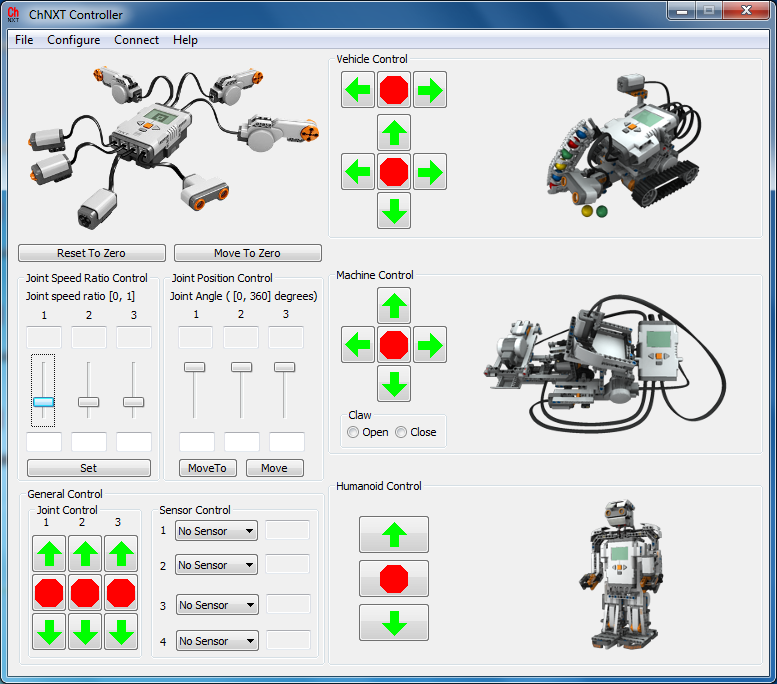
\includegraphics[height=4in]{figure/configuration/mainDlg.png}
    \caption{The main dialog of the ChNXT Controller.\label{fig:main_dialog}}
  \end{center}
\end{figure}
%%%%% END OF FIGURE %%%%%

Then click the menu item "Configure $\rightarrow$ Configure Robot Bluetooth", as shown in Figure~\ref{fig:menu_config}.

%%%%% START OF FIGURE %%%%%
\begin{figure}[H]
  \begin{center}
    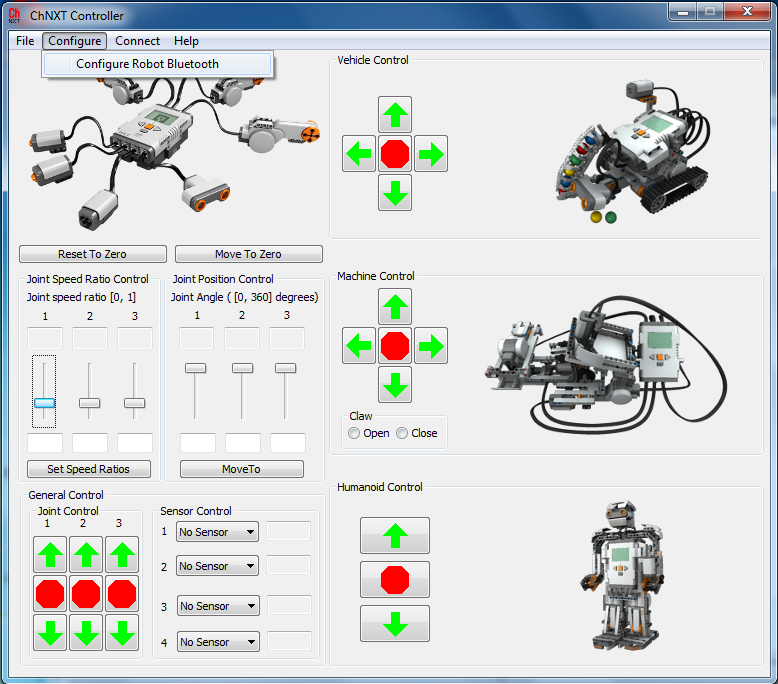
\includegraphics[height=3.4in]{figure/configuration/menuConfig.png}
    \caption{Configuring robot bluetooth connection.\label{fig:menu_config}}
  \end{center}
\end{figure}
%%%%% END OF FIGURE %%%%%

Now, the configuration dialog will appear on your screen, which is titled as "Configure Robot Bluetooth", as shown in 
Figure~\ref{fig:config_dialog}.

%%%%% START OF FIGURE %%%%%
\begin{figure}[H]
  \begin{center}
    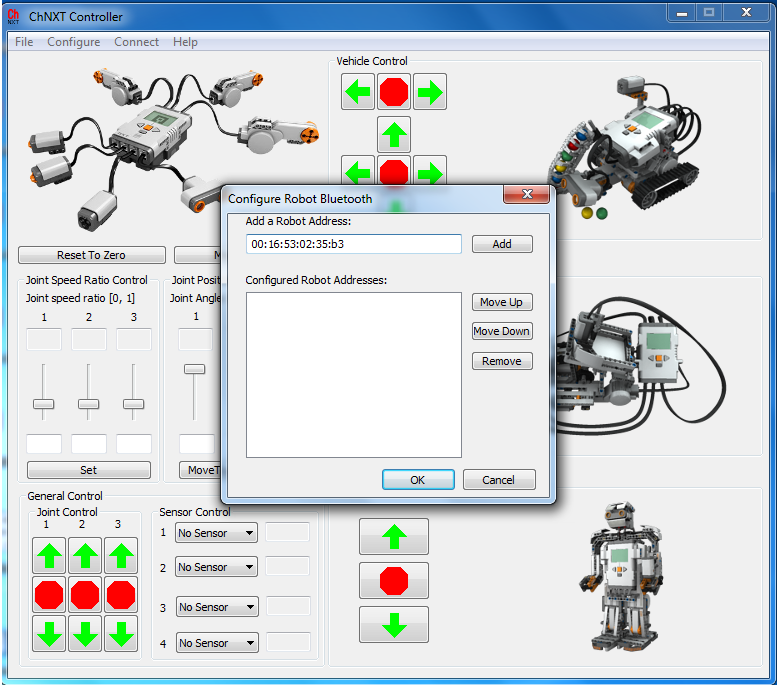
\includegraphics[height=3.4in]{figure/configuration/configDlg.png}
    \caption{The bluetooth configuration dialog.\label{fig:config_dialog}}
  \end{center}
\end{figure}
%%%%% END OF FIGURE %%%%%

In this configuration dialog, we can add robot bluetooth addresses to the list of currently know robot bluetooth addresses.
To add an address, first type in the address in the text box on the top of the dialog, as shown in Figure~\ref{fig:add_address}.

%%%%% START OF FIGURE %%%%%
\begin{figure}[H]
  \begin{center}
    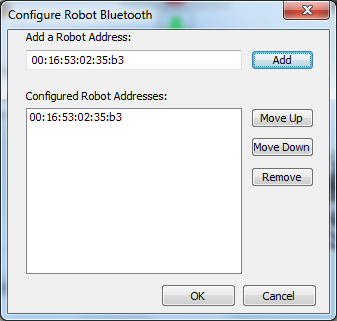
\includegraphics[height=2.5in]{figure/configuration/addBTaddress.png}
    \caption{Adding the robot bluetooth address in the dialog window.\label{fig:add_address}}
  \end{center}
\end{figure}
%%%%% END OF FIGURE %%%%%

Then, click he "Add" button. The newly added address will appear in the list of known addresses and click "Ok" button to exit 
the configuration dialog. With this method, you can add more bluetooth addresses. Also, the "Move Up" button, "Move Down" 
button, and the "Remove" button can be used to manage your bluetooth address list.

\subsection{Connecting and Disconnecting to NXTs from the ChNXT Controller}
%%%%% START OF FIGURE %%%%%
\begin{figure}[!h]
  \begin{center}
    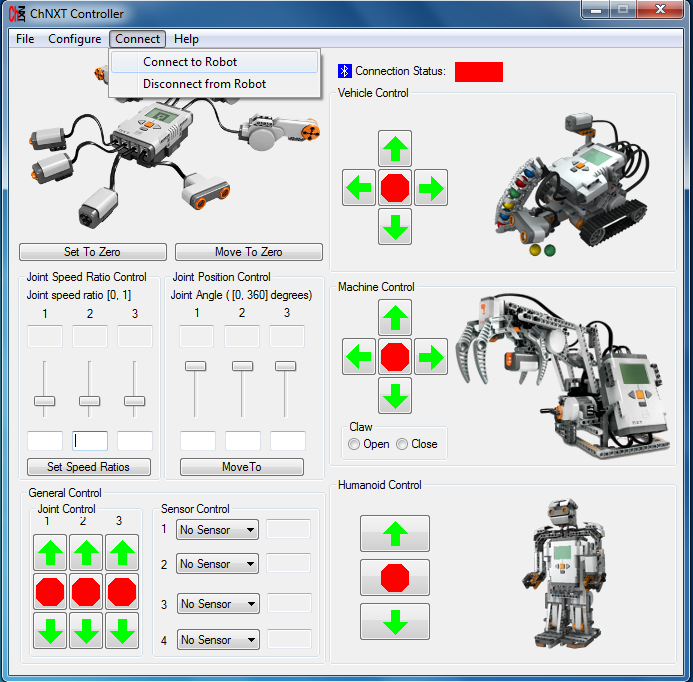
\includegraphics[height=3.5in]{figure/configuration/menuConnect.png}
    \caption{Connecting to and disconnecting from an NXT.\label{fig:menu_connect}}
  \end{center}
\end{figure}
%%%%% END OF FIGURE %%%%%

Once bluetooth addresses are added to the ChNXT Controller, you are now able to connect to a NXT device by clicking on the 
"Connect $\rightarrow$ Connect to Robot" menu item. Then the first NXT on the bluetooth address list will be connected and please make
sure the NXT is turned on, otherwise the connection will fail. Also, by clicking "Connect $\rightarrow$ Disconnect from Robot" menu 
item, the computer will disconnect from the remote device. Those two menu items are as shown in Figure~\ref{fig:menu_connect}.\\

Please note that in order to run a Ch program that controls NXTs, the NXTs should not currently be connected to any other
application, including the ChNXT Controller, other Ch Programs, and other programs on other devices.\\

Furthermore, the Bluetooth devices have a maximum limit of connected devices. The maximum limit is 7 devices connected 
simultaneously.

\newpage
\section{Getting Started with Ch NXT Package}
In this chapter, the basics of controlling an NXT via Ch program will be discussed. The basics are including
control an NXT joints, setup an NXT sensor, and also get information from joints and sensors. The basic structure 
of a Ch NXT robot program is shown in the flow diagram in Figure \ref{fig_NXT_pstruc} below.\\

%%%%% START OF FIGURE %%%%%
\begin{figure}[h!]
  \begin{center}
    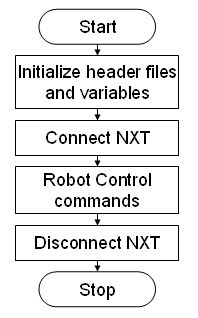
\includegraphics[height=3in]{figure/mindstorm/NXT_pstruc.png}
    \caption{Flow Diagram of a basic NXT program\label{fig_NXT_pstruc}}
  \end{center}
\end{figure}
%%%%% END OF FIGURE %%%%%

Also, to successfully control the Mindstorm NXT using Ch, it is important to practice good coding habits. 
The format of the Ch Mindstorm code is very similar to how a normal C code would be written, with the
inclusion of some Ch specific functions and header files that are used to connect and control the NXT. To 
help the user become acquainted with the Ch NXT programs, sample programs will be presented in this 
section to illustrate the basics and minimum requirements of a Ch NXT control program. The sample programs
are located at \texttt{CHHOME/package/chnxt/demos}, where \texttt{CHHOME} is the Ch home directory, such as
\texttt{C:$\backslash$Ch} for Windows. Therefore, for Windows, the demos are located at 
\texttt{C:$\backslash$Ch$\backslash$package$\backslash$chnxt$\backslash$demos} by default.

\subsection{\label{sec:basic_demo}A Basic Ch NXT Program}
The first demo presents a minimal program which connects to a Lego Mindstorms NXT and moves joints 2 and 3.

\subsubsection*{Source Code}
%%%%%%%%%%%%%%%%%%%%%% Begin of start.ch %%%%%%%%%%%%%%%%%%%%%%%%%%%%%%%%%
\begin{comment}
\begin{Program}[H]
    {\small\verbatiminput{demos/basic/start.ch}}
    \caption{\texttt{start.ch} Source Code\label{prog_start.ch}}
\end{Program}
\end{comment}

\begin{Program}[H]
    {\small\verbatiminput{demos/basic/start.ch_part1}}
    \caption{\texttt{start.ch} Source Code\label{prog_start.ch}}
\end{Program}
\addtocounter{Program}{-1}
\begin{Program}[H]
    {\small\verbatiminput{demos/basic/start.ch_part2}}
    \caption{\texttt{start.ch} Source Code (Continued.)\label{prog_start.ch}}
\end{Program}
%%%%%%%%%%%%%%%%%%%%% End of start.ch %%%%%%%%%%%%%%%%%%%%%%%%%%%%%%%%%%%%%%%

\subsubsection*{Header files}
The beginning of every program will include related header files. Each header file imports functions used for
a number of tasks, such as displaying message on the screen or controlling the Lego Mindstorms NXT. The header
file \texttt{nxt.h}, which contains all \texttt{ChNXT} class and other related functions for controlling the NXT, 
should be included in each Ch NXT program.
\begin{verbatim}
#include <nxt.h>
\end{verbatim}

\subsubsection*{Initialization}
The following line initializes a new variable named nxt which represents the remote Lego Mindstorm NXT which
we wish to control. The special variable is actually an instance of the ChNXT class, which contains its own
set of functions called "methods", "menber functions", or simply "functions".
\begin{verbatim}
ChNXT nxt;
\end{verbatim}

The next line,
\begin{verbatim}
nxt.connect();
\end{verbatim}

will connect our computer to the remote NXT, which is related to the new variable \texttt{nxt}.\\

Another way to get connected with the NXT is using the function \texttt{connectWithAddress()}, and the usesage
is as following:

\begin{verbatim}
nxt.connectWithAddress("11:22:33:44:55:66");
\end{verbatim}

The string \texttt{"11:22:33:44:55:66"} represents the Bluetooth address of the Lego Mindstorms NXT you wish 
to connect. Detailed documentation for \texttt{connect()} \texttt{connectWithAddress()} are presented in 
Appendix \ref{sec:chnxt_api} on page \pageref{sec:chnxt_api}. The next line,

\begin{verbatim}
nxt.moveToZero();
\end{verbatim}

uses the function \texttt{moveToZero()} which is a member function of class \texttt{ChNXT}. The function causes
all joints of the connected NXT move to zero position, which means the absolute angle will be all zero.\\

The next line of code will cause all joints of the connected NXT rotate 360 degrees.

\begin{verbatim}
nxt.move(360, 360, 360);
\end{verbatim}

The member function \texttt{move()} expects input angles in degrees. If you want to use angles in radians, the 
conversion need to be done via the function \texttt{rad2deg()}. The function is implemented in Ch with code

\begin{verbatim}
#include <math.h> /* For M_PI */
double rad2deg(double radians){
    double degrees;
    degrees = radians * 180.0 / M_PI;
    return degrees;
}
\end{verbatim}

If desired, values in radians may also be converted to degrees using the counterpart function, \texttt{deg2rad()}.
Detailed information for function \texttt{rad2deg()} and function \texttt{deg2rad()} can be found in Appendix 
\ref{sec:ultility_functions} on page \pageref{sec:ultility_functions}.\\

\subsection{\label{sec:setzero_demo}Setting the Zero Positions for NXT Joints}
In last section, we introduced a very basic demo of Ch NXT programs. In this section, another simple demo
will be presented to illustrated how to set absolute zero positions for joints.

\subsubsection*{Source Code}
\begin{Program}[H]
    {\small\verbatiminput{demos/basic/setZero.ch}}
    \caption{\texttt{setZero.ch} Source Code\label{prog_setZero.ch}}
\end{Program}

\subsubsection*{Explanation}
The first several lines of the code,\\

\begin{verbatim}
#include <nxt.h>

ChNXT nxt;

/* Connect to the NXT */
nxt.connect();
\end{verbatim}

initializes the program, declares the variable and connects to the remote device. The next line,

\begin{verbatim}
/* Set new zero positions */
nxt.setJointZero(NXT_JOINT1);
\end{verbatim}

sets \texttt{NXT\_JOINT1} to the new zero position. In order to set new zero positions, user should 
move the desired position before calling the function \texttt{setJointZero()}. The function \texttt{setJointZero()} 
can only set zero position for one joint. The argument it takes is the target joint. Another function called 
\texttt{setJointZeros()}, which takes no arguments, can set new zero positions for all joints. The next line,

\begin{verbatim}
/* Move to zero */
nxt.moveToZero();
\end{verbatim}

makes all joints move to new zero positions. The last part of the code,

\begin{verbatim}
/* Disconnect from NXT */
nxt.disconnect();
\end{verbatim}

disconnects from the NXT.

\subsection{\label{sec:speed_demo}Controlling the Speed of NXT Joints}
Now that we have already discussed how to include related header files, define variables for the program, 
get connected with/disconnect from the NXT and also set zero positions NXT joints. In this section, we will 
present a demo program, \texttt{setSpeedRatios.ch}, to illustrate how to set speed ratios for the joints of NXT.

\subsubsection*{Source Code}
\begin{Program}[H]
    {\small\verbatiminput{demos/basic/setSpeedRatios.ch}}
    \caption{\texttt{setSpeedRatios.ch} Source Code\label{prog_setSpeedRatios.ch}}
\end{Program}

\subsubsection*{Explanation}
The fisrt several lines,

\begin{verbatim}
#include <nxt.h>
ChNXT nxt;

/* Connect to the paired NXT */
nxt.connect();
\end{verbatim}

initializes the program, variable, and connect to the NXT. The next three lines,

\begin{verbatim}
/* set speed ratios */
nxt.setJointSpeedRatios(0, 0.4, 0.4);
nxt.setJointSpeedRatio(NXT_JOINT1, 0.5);
\end{verbatim}

sets the speed ratios setting for all joints on the NXT. The function \texttt{setJointSpeedRatios()} sets 
the speed ratio for \texttt{NXT\_JOINT1} as 0 and sets the speed ratios for \texttt{NXT\_JOINT2} and 
\texttt{NXT\_JOINT3} as 0.4. The function \texttt{setJointSpeedRatio()}, which can only set speed ratio
for one joint, sets the speed ratio for \texttt{NXT\_JOINT1} as 0.5.\\


The next two lines,

\begin{verbatim}
/* make NXT joints move */
nxt.move(360, 360, 360)
\end{verbatim}

makes three joints of NXT move at setted speed ratios. The usage of the function \texttt{move()} is just 
as the demo discussed in section~\ref{sec:basic_demo} on page \pageref{sec:basic_demo}.\\

The last part of the code,

\begin{verbatim}
/* disconnect */
nxt.disconnect();
\end{verbatim}
disconnects from the NXT.\\

\subsection{\label{sec:move_demo}Making NXT Joints Move}
Now that we have already discussed connect/disconnect and set speed ratios for joints, this section will presents a full
series of moving functions.

\subsubsection{A Demo Program for Movement Functions}
In this section, a simple demo program will be presented to illustrate the series functions of moving NXT joints.

\subsubsection*{Source Code}
\begin{comment}
\begin{Program}[H]
    {\small\verbatiminput{demos/basic/move.ch}}
    \caption{\texttt{move.ch} Source Code\label{prog_move.ch}}
\end{Program}
\end{comment}

\begin{Program}[H]
    {\small\verbatiminput{demos/basic/move.ch_part1}}
    \caption{\texttt{move.ch} Source Code\label{prog_move.ch}}
\end{Program}
\addtocounter{Program}{-1}
\begin{Program}[H]
    {\small\verbatiminput{demos/basic/move.ch_part2}}
    \caption{(Continued.)\label{prog_move.ch}}
\end{Program}

\subsubsection*{Explanation}
The first part of code,

\begin{verbatim}
#include <nxt.h>
ChNXT nxt;

/* Connect to the NXT */
nxt.connect();

/* Set speed ratios */
nxt.setJointSpeedRatios(0.5, 0.5, 0.5);
\end{verbatim}

initializes the program, connects to the NXT and sets speed ratios for joints. The next couple lines,

\begin{verbatim}
/* move joint to zero position */
nxt.moveToZero();
\end{verbatim}

moves the joint to the absolute zero positions for all joints. The function \texttt{setJointZero()} and \texttt{setJointZeros()} 
are used to set joints absolute positions. Detailed information for these two functions can be found in Appendix \ref{sec:chnxt_api}
. The next four lines,
% begin comment
\begin{comment}
\begin{verbatim}
/* rotate a joint continuously */
nxt.moveJointContinuousNB(NXT_JOINT1, NXT_FORWARD);
delay(5);
nxt.stopOneJoint(NXT_JOINT1);
\end{verbatim}
rotates \texttt{NXT\_JOINT1} continuously until a stop function is called. The stop function here we used is 
\texttt{stopOneJoint()}, which can only stop the specified joint.Other two stop functions are \texttt{stopTwoJoints()} 
and \texttt{stopAllJoints()}, which stops two joints and all joints respectively. The next four lines,
\end{comment}
% end comment
\begin{verbatim}
/* move a joint by user specified angle */
nxt.moveJoint(NXT_JOINT1, 360);

/* move a joint to absolute angle */
nxt.moveJointTo(NXT_JOINT1, 360);
\end{verbatim}
includes two functions \texttt{moveJoint()} and \texttt{moveJointTo}, which makes one joint move a specified angle
relatively and absolutely respectively. Similarly, the next four lines,
\begin{verbatim}
/* move all joints by specified angles */
nxt.move(180, 360, 360);

/* move all joints to absolute angles */
nxt.moveTo(360, 360, 360);
\end{verbatim}
includes functions \texttt{move()} and \texttt{moveTo}, which makes all joints move specified angles relatively and absolutely respectively. The last part,
\begin{verbatim}
/* disconnect from NXT */
nxt.disconnect();
\end{verbatim}
disconnects from an NXT device as all demos discribed in previous sections.

\subsubsection{\label{sec:block_nonblock}Blocking and Non-Blocking Functions}
The movement functions described in previous demo are all blocking ones. Once the blocking movement functions
are called, the functions will hang, or "blocking", until all the joints have stopped moving.
However, the movement functions also have "non-blocking" version, which means the function returns 
immediately and the function \texttt{moveWait()} can be used to wait for the movement stopping. \texttt{NB} at
the end of non-blocking functions indicates that the functions are non-blocking version, such as \texttt{moveNB()}. 
A simple example will be presented in the following.\\

\noindent
\textbf{Example}
\begin{verbatim}
#include <nxt.h>

ChNXT nxt;

/* Connect to the NXT */
nxt.connect();

/* Non-blocking Function */
nxt.moveJointNB(NXT_JOINT1, 360);
printf("This message will be printed on \
        the screen when joint1 is moving.\n");
nxt.moveWait();

/* Blocking Function */
nxt.moveJoint(NXT_JOING1, 360);
printf("This message will be printed on \
        the screen after joint1 stopped moving.\n");

/* Disconnect from the NXT */
nxt.disconnect();
\end{verbatim}

\noindent
\textbf{Explanation}\\
\newline
The first several lines,
\begin{verbatim}
#include <nxt.h>

ChNXT nxt;

/* Connect to the NXT */
nxt.connect();
\end{verbatim}
just like all NXT programs, initializes the program and connects to the NXT. Then the next part,
\begin{verbatim}
/* Non-blocking Function */
nxt.moveJointNB(NXT_JOINT1, 360);
printf("This message will be printed \
        on the screen when joint1 is moving.\n");
nxt.moveWait();
\end{verbatim}
is showing the non-blocking function \texttt{moveJointNB()}. The function \texttt{printf()} will
print a message onto the screen during the joint1 is moving. However, the blocking part below,
\begin{verbatim}
/* Blocking Function */
nxt.moveJoint(NXT_JOING1, 360);
printf("This message will be printed on \
        the screen after joint1 stopped moving.\n");
\end{verbatim}
will print out the message after the function \texttt{moveJoint()} finished, which means the
joint1 stops moving. Most moving functions have both blocking and non-blocking version. However,
there are still some exceptions. The function \texttt{moveJointContinuousNB()} and function
\texttt{moveContinuousNB()} have only non-blocking version and the function \texttt{moveContinuousTime()}
only has blocking version. In table~\ref{tab:block_nonblock}, we list all blocking functions and their 
corresponding non-blocking functions.
\begin{center}
    \begin{longtable}{ p{7cm}p{7cm}}
\caption{Block and Non-block Functions\label{tab:block_nonblock}}\\
\hline
Block Functions & Non-block Functions\\
\hline
\texttt{moveJoint()}            &\texttt{moveJointNB()}\\
\texttt{moveJointTo()}          &\texttt{moveJointToNB()}\\
\texttt{move()}                 &\texttt{moveNB()}\\
\texttt{moveTo()}               &\texttt{moveToNB()}\\
\texttt{moveToZero()}           &\texttt{moveToZeroNB()}\\
\texttt{vehicleRollForward()}      &\texttt{vehicleRollForwardNB()}\\
\texttt{vehicleRollBackward()}     &\texttt{vehicleRollBackwardNB()}\\
\texttt{vehicleRotateLeft()}       &\texttt{vehicleRotateLeftNB()}\\
\texttt{vehicleRotateRight()}      &\texttt{vehicleRotateRightNB()}\\
\hline
\end{longtable}
\end{center}

Also, detailed information for both blocking and non-blocking versions of movement functions can be found in Appendix 
\ref{sec:chnxt_api} on page \pageref{sec:chnxt_api}.

\subsection{Retrieving a Joint Angle}
This demo presents how to get a joint current angle in a Ch NXT program. The angle is the absolute postion in degrees.

\subsubsection*{Source Code}
\begin{Program}[H]
    {\small\verbatiminput{demos/basic/getJointAngle.ch}}
    \caption{\texttt{getJointAngle.ch} Source Code\label{prog_getJointAngle.ch}}
\end{Program}

\subsubsection*{Explanation}
As all programs, the first part of this program,
\begin{verbatim}
#include <nxt.h>
ChNXT nxt;

/* Connect to a NXT */
nxt.connect();
\end{verbatim}
\noindent
is to include the related header files, which is \texttt{nxt.h} in this program, to initialize variable and 
to connect to the remote NXT device. The next three lines of the code,
\begin{verbatim}
/* Get the joint angle of the first joint */
double angle;
nxt.getJointAngle(NXT_JOINT1, angle)
\end{verbatim}
\noindent
retrieves the current angle of joint 1. \texttt{NXT\_JOINT1} is an enumerated value defined in the header
file \texttt{nxt.h}. Detailed information for all enumerated values defined in \texttt{nxt.h} can be found
in Appendix \ref{sec:datatypes} on page \pageref{sec:datatypes}. Finally, the last part of the program,
\begin{verbatim}
/* Print out the joint angle */
printf("The current joint angle for joint 1 is %lf degrees.\n", angle)
\end{verbatim}
\noindent
prints the value of the variable onto the screen.\\

\subsection{\label{setSensor_demo}Setting Sensors for NXT}
We have finished discussing the connection and movement functions in previous sections and In this section,
we will start to discuss how to use sensors of NXT. The following demo code will present how to setup a sensor
for NXT and how to get values collected by the sensor from the NXT.
\subsubsection*{Source Code}
\begin{Program}[H]
    {\small\verbatiminput{demos/basic/sensor.ch}}
    \caption{\texttt{sensor.ch} Source Code\label{prog_sensor.ch}}
\end{Program}
\subsubsection*{Explanation}
The first part of the code,
\begin{verbatim}
#include <nxt.h>

ChNXT nxt;

/* Setup sensors and check sensor connection */
int status1=2, status2=2;

/* Variables to store values gotten from NXT */
int touchValue, ultraValue;

/* Connect to NXT */
nxt.connect();
\end{verbatim}
initializes the program, declares the variables and connects to the NXT. Here, we declared two more sets of variables, 
where one set is used to check the connection status of sensors and another set is used to store the values collected 
by sensors. The next part of code,
\begin{verbatim}
/* Save status of NXT_SENSORPORT1, and NXT_SENSORPORT4 */
status1 = nxt.setSensor(NXT_SENSORPORT1, 
            NXT_SENSORTYPE_TOUCH, NXT_SENSORMODE_BOOLEANMODE);

status2 = nxt.setSensor(NXT_SENSORPORT4,
            NXT_SENSORTYPE_ULTRASONIC, NXT_SENSORMODE_RAWMODE);
\end{verbatim}
\noindent
setups two sensors for the connected NXT. The function we used to setup sensors is \texttt{setSensor()}, 
which takes three arguments. The first argument represents the port number on the NXT, 
which is in type \texttt{nxtSensorPort\_t}. The second argument the function takes is the type of a sensor,
which is in type \texttt{nxtSensorType\_t}. And the last argumentis the working mode of a sensor, 
which is in type \texttt{nxtSensorMode\_t}. Detailed information for the three variable types can be found 
in Appendix \ref{sec:datatypes}. The next several lines,
\begin{verbatim}
/* Check connection status sensors connection */
if(status1) {
    printf("Fail to setup sensors.\n");
    exit(-1);
}

if(status2) {
    printf("Fail to setup sensors.\n");
    exit(-1);
}
\end{verbatim}
checks the status of each sensor to see if they were setupped correctly. If fail to setup sensors, 
the program will exit automatically. The function \texttt{setSensor()} returns 1 means success. The next part of code,
\begin{verbatim}
/* get values collected by sensors from NXT */
nxt.getSensor(NXT_SENSORPORT1, touchValue);
nxt.getSensor(NXT_SENSORPORT4, ultraValue);
\end{verbatim}
gets the collected values from the NXT by using the function \texttt{getSensor()}. In order to use the function, 
two arguments are neccessary. One is the sensor port in type \texttt{nxtSensorType\_t}. Another argument is the 
address of the variable used to store value gotten from the NXT. The last part,
\begin{verbatim}
/* display the values we got onto the screen */
printf("Touch sensor: %d\n", touchValue);
printf("Ultrasonic sensor: %d\n", ultraValue);

/* disconnect */
nxt.disconnect();
\end{verbatim}
\noindent
displays the values gotten from the NXT onto the screen and the disconnects from the NXT.

\newpage
% Controlling a NXT Vehicle %
\section{Controlling a NXT Vehicle}
%%%%% START OF FIGURE %%%%%
\begin{figure}[h!]
  \begin{center}
    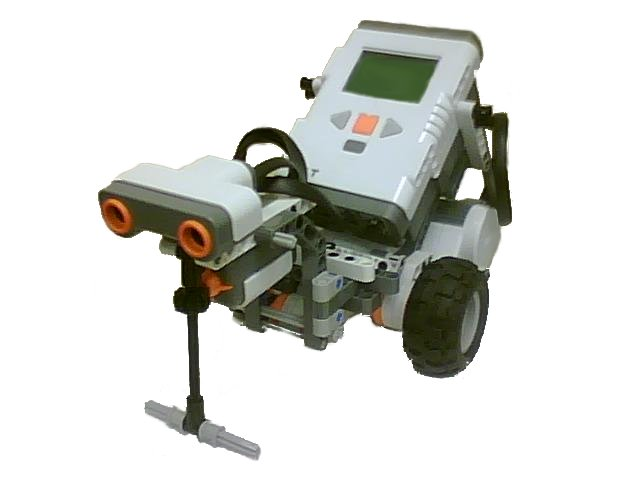
\includegraphics[height=3in]{figure/mindstorm/NXT_vehicle.png}
    \caption{NXT Vehicle\label{fig_NXT_vehicle}}
  \end{center}
\end{figure}
%%%%% END OF FIGURE %%%%%

\noindent
The NXT comes with three actuator output ports and the actuators available are the NXT motors. 
Normaly, you can only control the speed and direction of the connected motors. For a two wheeled NXT 
vehicle, there are two ways that the NXT vehicle can be controlled.  In addition to moving the NXT by
controlling the individual motors as shown in Figure \ref{fig_NXT_vehicle}, you can also use a set of
Ch mindstorm functions writen specificly to control an NXT vehicle. The diagram of the vehicle and 
the motor ports is shown in Figure \ref{fig_NXT_vehport}. When controlling the individual motors, you
would need to define the speed and direction of each motor.  The functions in the following examples 
require only a speed. In this section, we will show a basic Ch NXT program to move the robot forward.
Please make sure your NXT vehicle are configured according to to Figure \ref{fig_NXT_vehport} to run 
our demonstration programs.\\
%%%%% START OF FIGURE %%%%%
\begin{figure}[h]
  \begin{center}
    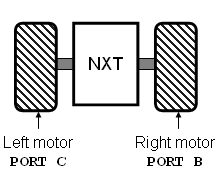
\includegraphics[height=2in]{figure/mindstorm/Vehicle.png}
    \caption{Motor configuration of the NXT Vehicle \label{fig_NXT_vehport}}
  \end{center}
\end{figure}
%%%%% END OF FIGURE %%%%%
\subsection{How to make your NXT move forward}
To help user become acquainted with the Ch NXT package, the example \verb+vehicleRollForward.ch+ will
be presented in the following section to illustrate the basics and minimum requirements of a Ch NXT 
control program. The code can be written using C or Ch syntax. For simplicity, the following code is 
presented as a Ch program.
%%%%%%%%%%  program of forward.ch %%%%%%%%%%%%%
\begin{Program}[H]
    {\small\verbatiminput{demos/vehicle/forward.ch}}
    \caption{\texttt{forward.ch} Source Code\label{prog_forward.ch}}
\end{Program}

\subsubsection{Initialization}
In the beginning of a Ch Mindstorms NXT program or any C program, you must include proper header 
files to run the program properly. Without proper header files, the program will not have the 
specific libraries or source codes to run the program. Essential header files for the NXT includes:
\begin{verbatim}
#include <nxt.h>
\end{verbatim}
\noindent
The \verb+nxt.h+ is the essential header file for Ch NXT control functions and variables.  

\subsubsection{Connect the NXT and Checking Connection Status}
The NXT status, sensor/encoder data, and input/output protocols are stored in a C++ class called 
\verb+ChNXT+. This class must be created in every NXT program in order to connect. Therefore, in the 
beginning of your code, you must define a \verb+ChNXT+ class and use the \verb+connect()+ function to
connect to the NXT. The \verb+connect()+ function will return a 1 if no connection is established, so
you will have to terminate your program if no connection is established. An example of how to create 
the \verb+class+ and how to retrieve data are shown below:
\begin{verbatim}
ChNXT nxt;

/* Check status of NXT connection */
if (nxt.connect()){
    printf("Error: Cannot connect to Lego Mindstorm NXT.\n");
    exit(-1);
}
\end{verbatim}
The line \verb+ChNXT nxt;+ creates the class \verb+nxt+ that is used to store data and control the 
NXT robot. The function \verb+nxt.connect()+ called in the if statement is used to terminate the 
program in the event no connection is established. The \verb+printf()+ is included to print out an 
error message if \verb+nxt.connect+ fails. To end the program if connection fails, the function 
\verb+exit()+ is used. The use of \verb+exit(-1)+ is similar to the C function \verb+return 0;+, that 
can be used when no \verb+main()+ function is present.
%\subsection{Set the Joints' Speed}
%After creating a connection with the NXT, you can begin your program to control the NXT. Before make 
%joints move, the speed of three joints has to be set by using the function \verb+setJointSpeed()+ to 
%setup a single joint or by using the function \verb+setJointSpeedRatios()+ to setup speed for all three 
%joints. However, the speed of the motors are limited, and can only be set from 1 to 100. The following 
%shows how to setup speed for joints of Lego Mindstorms:

%\begin{verbatim}
%    /* setup speed for a single joint */
%    nxt.setJointSpeed(NXT_JOINT1, 50);
%
%    /* setup speed for all joints */
%    nxt.setJointSpeedRatios(20, 40, 40);
%\end{verbatim}

% END OF SET SPEED %
%\newline
%\\
\subsubsection{Moving the Robot Forward}
After estabilishing the connection between a computer and an NXT, you can move the NXT 
vehicle forward by using the \verb+vehicleRollForward()+. After using the 
\verb+vehicleRollForward()+ function, the program will wait for the motion stopping. 
Figure \ref{fig_NXT_forward} shows the NXT vehicle moving forward by actuating both wheels 
forward with the same speed ratio, which is how the function \verb+vehicleRollForward()+ 
works. By default, the ports for the two wheels on the NXT are \textsc{NXT\_JOINT2} and 
\textsc{NXT\_JOINT3}.\\
\\
%%%%% START OF FIGURE %%%%%
\begin{figure}[h]
  \begin{center}
    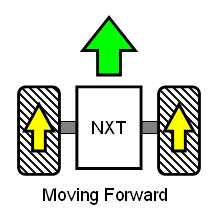
\includegraphics[height=2in]{figure/mindstorm/Vehicle_forward.png}
    \caption{Top-down view of NXT vehicle with two wheels\label{fig_NXT_forward}}
  \end{center}
\end{figure}
%%%%% END OF FIGURE %%%%%

\noindent
The following part is the maint code to make the NXT vehicle robot move forward in the 
program \verb+vehicleRollForward.ch+:
\begin{verbatim}
/* set speed ratio */
nxt.setSpeedRatios(0, 0.25, 0.25);

/* Move foward */
nxt.vehicleRollForward(360);
\end{verbatim}

\subsubsection{Ending your program}
After you finish your program, you must end your program properly by stopping all the motors and 
disconnect the NXT from your computer. You can stop the motors using the \verb+stopAllJoints()+ 
function, which stops all of the NXT motors. To disconnect the nxt, use the \verb+disconnect()+ 
function. For example:

\begin{verbatim}
/* Stop the motors */
nxt.stopAllJoints();
    
/* Disconnect NXT */
nxt.disconnect();
\end{verbatim}

\subsection{How to make your NXT move backward}
To make a NXT vehicle move backward, the function \texttt{vehicleRollBackward()} can be used. 
The function works smilarly to \texttt{vehicleRollForward()}, moving the robot backwards. The 
function works by actuationg both wheels backward at the same speed, as shown in Figure 
\ref{fig_NXT_backward}.\\
%%%%% START OF FIGURE %%%%%
\begin{figure}[h]
  \begin{center}
    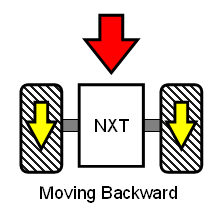
\includegraphics[height=2in]{figure/mindstorm/Vehicle_back.png}
    \caption{NXT vehicle moving backwards\label{fig_NXT_backward}}
  \end{center}
\end{figure}
%%%%% END OF FIGURE %%%%%
\noindent
Using our new function, we can add the following code fragment to our first program to make the robot
move backwards. The code fragment is shown below:
\begin{verbatim}
/* set speed ratio */
nxt.setJointSpeedRatios(0, 0.25, 0.25);

/* Move backward */
nxt.vehicleRollBackward(360);
\end{verbatim}
\noindent
The modified program is called: \verb+vehicleRollBackward.ch+.

%%%%%%%%%%%%%%%% how to make your NXT turn in place left/right %%%%%%%%%%
\subsection{How to make your NXT turn in place left/right}

To make your NXT vehicle turn or rotate in place, the NXT vehicle wheels must be spun in the opposite
direction at the same speed. For example, to rotate the NXT vehicle to the left, the right wheel must
be spun forward, while the left wheel spins at the same speed in reverse. Figure \ref{fig_NXT_360LR} 
shown below shows the NXT vehicle turning in place left or right by actuating the wheels in opposite 
direction.\\
%%%%% START OF FIGURE %%%%%
\begin{figure}[h]
  \begin{center}
    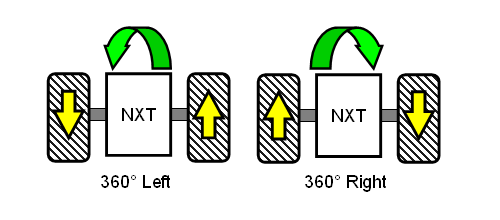
\includegraphics[height=2in]{figure/mindstorm/Vehicle_360LR.png}
    \caption{NXT vehicle turning 360 degrees \label{fig_NXT_360LR}}
  \end{center}
\end{figure}
%%%%% END OF FIGURE %%%%%

\noindent
To make the NXT rotate in place, we can use the functions \verb+vehicleRotateLeft()+ 
and \verb+vehicleRotateRight()+. An example of how to use the functions are shown below:
\begin{verbatim}
/* set speed ratio */
nxt.setJointSpeedRatios(0, 0.50, 0.50);
    
/* rotate left */
nxt.vehicleRotateLeft(360);

// or
    
/* set speed ratio */
nxt.setJointSpeedRatios(0, 0.50, 0.50);

/* rotate right */
nxt.vehicleRotateRight(360);
\end{verbatim}
\noindent
An example program is called: \verb+vehicleRotate.ch+.

%%%%%%%%%%%%%% Advance Mindstorm Motor Control %%%%%%%%%%%%%
\subsection{Advance Mindstorm Motor Control}
The previous section showed simplified controls for an NXT vehicle robot. To control 
alternate NXT designs, or to perform more advance movements with the NXT vehicle, the 
NXT motors must be controlled individually. The following sections shows how to control 
the individual motors, and how the previously presented NXT vehicle actions can be done 
by controlling the individual motors.

%%%%%%%%%%%%%%%%%% Motor Control Functions %%%%%%%%%%%%%%%%%
\subsubsection{Motor Control Functions}
The function that is used to control the NXT motors is \verb+moveJointContinuousNB()+. To use the 
function, you need the motor port and the move direction. The speed of the motors are limited, and 
can only ranged from 0 to 100. For the direction, the data type \texttt{nxtJointState\_t} is defined.
In the data type, there are two values indicate the move directions. One is call \texttt{NXT\_FORWARD},
which means the positive direction and the other is called \texttt{NXT\_BACKWARD} means the negative 
direction. The function is end with \texttt{NB}, which means the function is non-blocking one. Therefore,
you will need to use the \verb+delay()+ function to leave the motors on for the desired amount of the time. 
Otherwise, the program will go through the following statements directly. Due to the setup of the NXT vehicle, 
forward motion can be achieved by turning the motors on to the same speed ratio. For example:
\begin{verbatim}
/* set speed ratio */
nxt.setJointSpeedRatios(0, speedRatio, speedRatio);

/* Move foward */
nxt.moveJointContinuousNB(NXT_JOINT2, NXT_FORWARD);
nxt.moveJointContinuousNB(NXT_JOINT3, NXT_FORWARD);

/* Pause program for a while */
delay(5);
\end{verbatim}
\noindent
This will move the NXT vehicle forward at the value the variable speed was set to. To get the 
NXT vehicle to move in reverse, the same code can be used by changing the sign on speed in the 
function \verb+setJointSpeedRatios()+. The following shows the \verb+forwardBackward.ch+ 
rewritten to use the individual motor control.
%%%%%%%%%%%%  Begin of forwardBackward.ch %%%%%%%%%%%%%
\begin{Program}[H]
    {\small\verbatiminput{demos/vehicle/forwardBackward.ch}}
    \caption{\texttt{forwardBackward.ch} Source Code\label{prog_forwardBackward.ch}}
\end{Program}

\begin{comment}
\begin{Program}[H]
    {\small\verbatiminput{demos/vehicle/forwardBackward.ch_part1}}
    \caption{\texttt{forwardBackward.ch} Source Code\label{prog_forwardBackward.ch}}
\end{Program}
\addtocounter{Program}{-1}
\begin{Program}[H]
    {\small\verbatiminput{demos/vehicle/forwardBackward.ch_part2}}
    \caption{\texttt{forwardBackward.ch} Source Code (Continued.)\label{prog_forwardBackward.ch}}
\end{Program}
\end{comment}
%%%%%%%%%%%% End of forwardBackward.ch %%%%%%%%%%%%%%%%%%%%
%%%%%%%%%%%% Turning Using Single Motor Control %%%%%%%%%%%%
\subsubsection{Turning Using Single Motor Control}
Turning and rotation movements can also be achieved using the \verb+moveJointContinuousNB()+ 
functions. As previously discussed, to turn our NXT vehicle, one motor must be rotating at a 
faster speed then the other, or the motors must be spinning in the opposite direction. For 
the following discussion, Figures \ref{fig_NXT_360LR} maybe useful.\\

\noindent
To turn the NXT vehicle left, the right wheel must be moving faster in forward direction then the 
left wheel. If you want to move forward and turn left, let the left wheel move at 0.7 of the 
speed that the right wheel is set to. To implement it with the single motor control functions, you 
would do the following:
\begin{verbatim}
/* set speed ratio */
nxt.setJointSpeedRatios(0, speedRatio, 0.7*speedRatio);

/* Move foward-left */
nxt.moveJointContinuousNB(NXT_JOINT2, NXT_FORWARD);
nxt.moveJointContinuousNB(NXT_JOINT3, NXT_FORWARD);

/* Pause program for a while */
delay(5);
\end{verbatim}
\noindent
The value of 0.7 is somewhat arbitrary, and other constant values could be used to test the resulting
NXT vehicle response. The function \verb+vehicleRotateLeft()+ works similarly, instead setting the 
left wheel at the negative speed of the right wheel. An example is shown below:
\begin{verbatim}
/* set speed ratio */
nxt.setJointSpeedRatios(0, speedRatio, speedRatio);

/* Rotate left in place */
nxt.moveJointContinuousNB(NXT_JOINT2, NXT_FORWARD);
nxt.moveJointContinuousNB(NXT_JOINT3, NXT_BACKWARD);

/* Pause program for a while */
delay(5);
\end{verbatim}
\noindent
To make the functions \verb+vehicleRotateLeft()+ and \verb+vehicleRotateRight()+ work, you need to make
the speed ratio opposite. Once you understand how the single motor commands work, more advance movements
can be done, such as a move back and left motion. The single motor commands can also be used to add a 
third motor attachment to the NXT vehicle, or used to control alternate robot designs that move or act 
differently.\\
\newline

\noindent
One alternative approach to implementing turning is to increase the speed of a wheel, instead of 
decreasing a wheel speed. For example, to implement a left turn, we could increase the speed of 
the right wheel by multiplying by a constant, such as 1.2.  The resulting code would look like:

\begin{verbatim}
/* set speed ratios */
nxt.setJointSpeedRatios(0, 1.2*speedRatio, speedRatio);

/* Move foward-left */
nxt.moveJointContinuousNB(NXT_JOINT2, NXT_FORWARD);
nxt.moveJointContinuousNB(NXT_JOINT3, NXT_FORWARD);

/* Pause program for a while */
delay(5);
\end{verbatim}

\noindent
While this would work for slower motor speeds, a bug would occur if the NXT vehicle speed was 
set too high. Can you spot why? As previously discussed, the valid motor speed ratio for NXT 
motors are between 0 to 1. If the speed variable is set to 1, the command to control 
the left motor (NXT\_JOINT3) will function correctly. The right motor (NXT\_JOINT2) will 
recieve a command telling it to set the motor speed to 1.2 x 1 = 1.2. This is an invalid motor 
command, and if you tried to run it on the NXT, it will cause the motor to reverse direction, 
making the NXT vehicle turn right instead of left. It is important to be watchful of these 
type of errors while writing code to control the NXT.\\

\subsubsection{Manual Real Time Control Program}
Manual real time control program allows you to control your NXT vehicle with your keyboard like a 
remote control. For a manual control program, a user interface is usually used to display all the 
possible option that a user can input into the program. The user interface allow the user to know how
to control the NXT's motion. The NXT vehicle RTC program prints out a user interface for the user to 
use while executing the program. Figure \ref{fig_NXT_GUI} is the user interface of the NXT vehicle 
RTC program.\\
%%%%% START OF FIGURE %%%%%
\begin{figure}[h]
  \begin{center}
    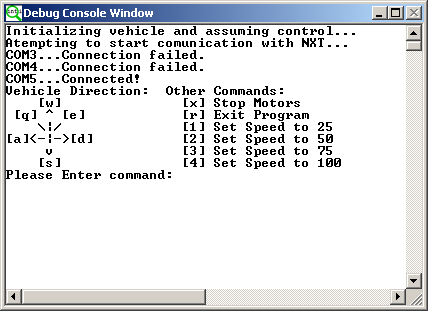
\includegraphics[height=3in]{figure/mindstorm/RTC_GUI.png}
    \caption{NXT vehicle RTC User Interface \label{fig_NXT_GUI}}
  \end{center}
\end{figure}
%%%%% END OF FIGURE %%%%%
\\
In Figure \ref{fig_NXT_GUI}, the user interface of the NXT vehicle RTC program display all the 
possible key that the user can use. In addition, the user interface also indicate the functionality 
of the key that is being pressed. When a specific key is pressed during the execution of the NXT 
vehicle RTC program, the program uses a \verb+if-else if-else+ statement to performs a fragment of code that
send commands to the NXT.
For example:\\
\begin{itemize}
\item The key \verb+"w"+ is to control the NXT to move forward.
\item The key \verb+"s"+ is to control the NXT to move backward.
\item The key \verb+"a"+ is to control the NXT to turn left.
\item The key \verb+"d"+ is to control the NXT to turn right.
\item The key \verb+"x"+ is to stop the NXT motors.
\item The key \verb+"1"+ is to set the NXT motor speed ratio from 0.25.
\item The key \verb+"2"+ is to set the NXT motor speed ratio from 0.5.
\item The key \verb+"3"+ is to set the NXT motor speed ratio from 0.75.
\item The key \verb+"4"+ is to set the NXT motor speed ratio from 1.
\item The key \verb+"r"+ is to exit the manual RTC program.
\end{itemize}

\noindent
In the robot control code block, a while loop is implemented to allow the user to control the NXT
continuously until the program is terminated. Within the while loop, the program grabs the user's 
input and decide what to do with it using the \verb+switch+ and \verb+case+ statements. The whole 
NXT vehicle RTC program is shown in Program~\ref{prog_vehicle_rtc.ch}. Please make sure your NXT 
vehicle are configured according to to Figure \ref{fig_NXT_vehport} to run 
Program~\ref{prog_vehicle_rtc.ch}. In the rest of this section, we are going to explain the whole 
program in detail.

%%%%%%%%%%%%%%%% Begin of vehicle_rtc.ch %%%%%%%%%%%%%%%%%%%%%%%%%%%%%%%%%%
\begin{comment}
\begin{Program}[H]
    {\small\verbatiminput{demos/vehicle/vehicle_rtc.ch}}
    \caption{\texttt{vehicle\_rtc.ch} Source Code\label{prog_vehicle_rtc.ch}}
\end{Program}
\end{comment}

\begin{Program}[H]
    {\small\verbatiminput{demos/vehicle/vehicle_rtc.ch_part1}}
    \caption{\texttt{vehicle\_rtc.ch} Source Code\label{prog_vehicle_rtc.ch}}
\end{Program}
\addtocounter{Program}{-1}
\begin{Program}[H]
    {\small\verbatiminput{demos/vehicle/vehicle_rtc.ch_part2}}
    \caption{\texttt{vehicle\_rtc.ch} Source Code (Continued.)\label{prog_vehicle_rtc.ch}}
\end{Program}
\addtocounter{Program}{-1}
\begin{Program}[H]
    {\small\verbatiminput{demos/vehicle/vehicle_rtc.ch_part3}}
    \caption{\texttt{vehicle\_rtc.ch} Source Code (Continued.)\label{prog_vehicle_rtc.ch}}
\end{Program}
%%%%%%%%%%%%%%%%%%%%%% End of vehicle_rtc.ch %%%%%%%%%%%%%%%%%%%%%%%%%%%%%

\subsubsection*{Header files}
Similar to any C program, you will have to include necessary header files, which is described in the 
first four lines.
    
\begin{verbatim}
#include <conio.h>
#include <stdio.h>
#include <nxt.h>
\end{verbatim}

\begin{itemize}
\item The header \verb+conio.h+ provides a function for the program to detect a key press for the
\verb+-press a key-+ command.
\item The header \verb+stdio.h+ provides input and output function for the program. These input and 
output function allows the program to display output for the user or ask for the user input.
\item The header \verb+nxt.h+ provides the program with general functions of the Ch Mindstorm 
Control Package.
\end{itemize}

\subsubsection*{Declaring variables}
After including the headers, the C program will start the \verb+main()+ program.
Like any C programs, you must declare variables before you can use them.
On the top few lines of the \verb+main()+ program, variables are declared.
\begin{verbatim}
ChNXT nxt;

double speedRaio = 0.25;//speed ratio of the motors. (default to 0.25)

int quit = 0,           //used by quit case to exit the loop
    status1,            //used to check for errors
    status2;            //used to check for errors

char key = 'x',	        //stores the input from the user
     movemode = 'x';    //stores the last movement command
\end{verbatim}

\begin{itemize}
\item The \verb+ChNXT+ class stores the connection status, sensor data, and motor counter data of the
    NXT. Also, the class includes the functions for controling the NXT.
\item The double variable \verb+speedRatio+ stores the speed ratio of the motor.
\item The integer variable \verb+quit+ is used to check if the user wants to quit the program.
\item The integer variable \verb+status1+ and \verb+status2+ are used to check the sensor connection.
\item The character variable \verb+key+ stores the input from the user.
\item The character variable \verb+movemode+ stores the last command that the user used.
\end{itemize}

\subsubsection*{Checking connection}
After declaring variables, the connection of the NXT needs to be checked.
In the next 7 lines of the program, the program checks for the connection of the NXT to the computer.
If the NXT connection fails, the program will quit.

\begin{verbatim}
/* Connect to NXT */
printf("Initializing vehicle and assuming control...");
if (nxt.connect()){
    printf("\nPress any key to exit.\n");
    while (!_kbhit()); //wait for keypress
        exit(-1);
}
\end{verbatim}

\subsubsection*{User interface}
Before the beginning of the real time control, the user must be able to know the function of the key 
they are pressing. To do this, the program print out a user interface for the user to read. 
In segment of the Program~\ref{prog_ultrasonicsensor.ch} shown below, the NXT vehicle RTC program used \verb+printf()+ command is 
used to display the user interface for the user to read.
\begin{verbatim}
/* GUI display */
printf("Vehicle Direction:  Other Commands:");
printf("\n    [w]               [x] Stop Motors");
printf("\n [q] ^ [e]            [r] Exit Program");
printf("\n    \|/               [1] Set Speed Ratio to 0.25");
printf("\n[a]<-|->[d]           [2] Set Speed Ratio to 0.50");
printf("\n     v                [3] Set Speed Ratio to 0.75");
printf("\n    [s]               [4] Set Speed Ratio to 1\n");
printf("Please Enter command:");
\end{verbatim}

\subsubsection*{Real time control}
After completing the initiation of the code, which include adding header files, declaring variables,
checking connection, and displaying the user interface, the real time control of the NXT begins with 
the robot control code block. In the robot control code block, a while loop is implemented to allow 
the user to control the NXT continuously until the program is terminated. Within the while loop, the 
program grabs an input from the user, and then decide what to do with the input using the 
\verb+if-else if-else+ and \verb+case+ statement. A basic flow diagram of the control loop for the NXT 
vehicle RTC program is shown in Figure \ref{fig_RTC_controlloop} below.\\
    
\begin{figure}[h]
  \begin{center}
    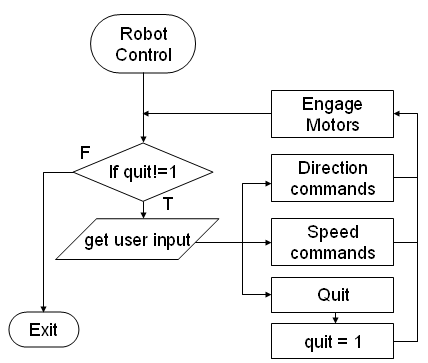
\includegraphics[height=2.4in]{figure/mindstorm/RTC_controlloop.png}
    \caption{NXT vehicle RTC Control Loop Flow Diagram \label{fig_RTC_controlloop}}
  \end{center}
\end{figure}

\noindent
The program fragment shown below shows the beginning and the end of the while loop for 
Program~\ref{prog_ultrasonicsensor.ch}:

\begin{verbatim}
while (quit != 1 ) {
    key = _getch();
    if(key == 'w'){
        ...
    }else if(key == 's'){
        ...
    }else{
        ...
    }
}
\end{verbatim}

\noindent
When the program reaches this stage, the real time control begins. The while loop allows the program 
to keep asking the user's input until the \verb+'r'+ key is pressed. When the \verb+'r'+ key is 
pressed, the program will set \verb+quit+ variable is set to 1, which allows the program to exit 
out of the while loop.\\ \\
\noindent
For first line of the while loop, the program use the \verb+_getch()+ command to obtain a user
input and store the user input to the variable \verb+key+. After obtaining the user's input in a 
variable, the program use a \verb+if-else if-else+ statement to check which key was pressed. Depending on 
what key was pressed, the program will run a fragment of code that sends commands to the NXT.

\subsubsection*{Directional commands}
The movements are controlled using the 'w', 's', 'a', and 'd' format. In Figure \ref{fig_NXT_GUI}, 
the user interface used arrows to indicate the movement direction and associate each direction with 
a specific key. The available buttons for movements are 'w', 's', 'a', 'd', 'q', 'e', and 'x'.
\\ \\
%%% case 'w' %%%
\noindent
When the key 'w' has been pressed, the \verb+if-else if-else+ statement will run the codes for the case 'w'.
The program fragment for case 'w' is shown below:
\begin{verbatim} 
if(key == 'w'){//up
    nxt.moveJointContinuousNB(NXT_JOINT2, NXT_FORWARD);
    nxt.moveJointContinuousNB(NXT_JOINT3, NXT_FORWARD);
    movemode = 'w';
}
\end{verbatim}
In case 'w', the program will run joints \verb+NXT_JOINT2+ and \verb+NXT_JOINT3+ forward at
the velocity \verb+speedRatio+. Next, 'w' key is stored in the variable \verb+movemode+, which will 
be used to indicate the current mode for NXT vehicle. Basically, the case 'w' will move the 
NXT vehicle forward at velocity \verb+speedRatio+.
\\ \\
%%% case 's' %%%
\noindent
When the key 's' has been pressed, the \verb+if-else if-else+ statement will run the codes 
for the case 's'. The program fragment for case 's' is shown below:
\begin{verbatim} 
else if(key == 's'){//down
    nxt.moveJointContinuousNB(NXT_JOINT2, NXT_BACKWARD);
    nxt.moveJointContinuousNB(NXT_JOINT3, NXT_BACKWARD);
    movemode = 's';
}
\end{verbatim}
In case 's', the program will run the joints \verb+NXT_JOINT2+ and \verb+NXT_JOINT3+ backward 
at the velocity \verb+speedRatio+. Next, 's' key is stored in the variable \verb+movemode+, 
which will be used to indicate the current mode for NXT vehicle. Basically, the case 's' will 
move the NXT vehicle backward with velocity \verb+speedRatio+.\\ 
\newline
%%% case 'a' %%%
\noindent 
When the key 'a' has been pressed, the \verb+if-else if-else+ statement will run the codes for the case 'a'.
The program fragment for case 'a' is shown below:
\begin{verbatim} 
else if(key == 'a'){//left
    nxt.moveJointContinuousNB(NXT_JOINT2, NXT_FORWARD);
    nxt.moveJointContinuousNB(NXT_JOINT3, NXT_BACKWARD);
    movemode = 'a';
}
\end{verbatim}
In case 'a', the program will actuate joint \verb+NXT_JOINT2+ forward at velocity \verb+speedRatio+ 
and actuate joint \verb+NXT_JOINT3+ backward at velocity \verb+speedRatio+. Next, 'a' key is stored in 
the variable \verb+movemode+, which will be used to indicate the current mode for NXT vehicle.\\ 
\newline
%%% case 'd' %%%
\noindent
When the key 'd' has been pressed, the \verb+if-else if-else+ statement will run the codes for the case 'd'.
The program fragment for case 'd' is shown below:
\begin{verbatim} 
else if(key == 'd'){//right
    nxt.moveJointContinuousNB(NXT_JOINT2, NXT_BACKWARD);
    nxt.moveJointContinuousNB(NXT_JOINT3, NXT_FORWARD);
    movemode = 'd';
}
\end{verbatim}
In case 'd', the program will actuate joint \verb+NXT_JOINT2+ backward at velocity \verb+speedRatio+ 
and actuate joint \verb+NXT_JOINT3+ forward at velocity \verb+speedRatio+. Next, 'd' key is stored in
the variable \verb+movemode+, which will be used to indicate the current mode for NXT vehicle.\\ 
\newline
%%% case 'q' %%%    
\noindent
When the key 'q' has been pressed, the \verb+if-else if-else+ statement will run the codes for the case 'q'.
The program fragment for case 'q' is shown below:
\begin{verbatim} 
else if(key == 'q'){//forward-left
    nxt.setJointSpeedRatios(0, speedRatio, 0.7*speedRatio);
    nxt.moveJointContinuousNB(NXT_JOINT2, NXT_FORWARD);
    nxt.moveJointContinuousNB(NXT_JOINT3, NXT_BACKWARD);
    movemode = 'q';
}
\end{verbatim}
In case 'q', the program will actuate joint \verb+NXT_JOINT2+ forward at velocity \verb+speedRatio+ 
and actuate joint \verb+NXT_JOINT3+ forward at velocity 0.7*\verb+speedRatio+. Next, 'q' key is 
stored in the variable \verb+movemode+, which will be used to indicate the current mode for NXT 
vehicle.\\ 
\newline
%%% case 'e' %%%
\noindent 
When the key 'e' has been pressed, the \verb+if-else if-else+ statement will run the codes for the case 'e'.
The program fragment for case 'e' is shown below:
\begin{verbatim} 
else if(key == 'e'){//forward-right
    nxt.setJointSpeedRatios(0, 0.7*speedRatio, speedRatio);
    nxt.moveJointContinuousNB(NXT_JOINT2, NXT_BACKWARD);
    nxt.moveJointContinuousNB(NXT_JOINT3, NXT_FORWARD);
    movemode = 'e';
}
\end{verbatim}
In case 'e', the program will actuate joint \verb+NXT_JOINT2+ forward at velocity 
0.7*\verb+speedRatio+ and actuate joint \verb+NXT_JOINT3+ forward at velocity 
\verb+speedRatio+. Next, 'e' key is stored in the variable \verb+movemode+, which will 
be used to indicate the current mode for NXT vehicle.\\ 
\newline
%%% case 'x' %%%
\noindent
When the key 'x' has been pressed, the \verb+if-else if-else+ statement will run the codes for the case 'x'.
The program fragment for case 'x' is shown below:
\begin{verbatim} 
else if(key == 'x'){//stop
    nxt.stopOneJoint(NXT_JOINT2);
    nxt.stopOneJoint(NXT_JOINT3);
    movemode = 'x';
}
\end{verbatim}
In case 'x', the program will set the motor in \verb+NXT_JOINT2+ and \verb+NXT_JOINT3+ to zero 
velocity, and then set the motor to off idle mode. Next, 'x' key is stored in the variable 
\verb+movemode+, which will be used to indicate the current mode for NXT vehicle.
Basically, the case 'x' stops the motor and keep it turned off until another key is pressed.

\subsubsection*{Speed control}
The speed of the motor is controlled by the number key '1', '2', '3', and '4'.
In Figure \ref{fig_NXT_GUI}, the user interface shows that each key has a specific speed ratio.
For example, key '1' indicates 0.25 speed ratio, and key '2' indicate 0.50 speed ratio.
As shown below, each of the key has its fragment of code.
\begin{verbatim}
else if(key == '1'){
    speedRatio = 0.25;
    ungetch(movemode);
}else if(key == '2'){
    speedRatio = 0.50;
    ungetch(movemode);
}else if(key == '3'){
    speedRatio = 0.75;
    ungetch(movemode);
}else if(key == '4'){
    speedRatio = 1;
    ungetch(movemode);
}
\end{verbatim}
\noindent
For each of the case, the fragment of code changes the variable \verb+speedRatio+ and performs an \verb+ungetch()+ command.
The \verb+ungetch()+ command allows the program run the mode that it was previously saved in the variable \verb+movemode+
before the speed keys are pressed. Basically, the speed keys allow the program to change the speed of the NXT motor without 
changing the movement mode that it was in.

\subsubsection*{Functions for other keys}
As mentioned before, the while loop allows the program to keep asking the user's input until the variable
\verb+quit+ is set to 1. To quit the while loop, we must have a special case that sets the variable \verb+quit+ to 1.
When the key 'r' is pressed, the \verb+if-else if-else+ statement will perform a fragment of code for case 'r'.
The program fragment for case 'r' is shown below:
\begin{verbatim}
else if(key == 'r'){//quit
    printf("\nExiting program.\n");
    quit = 1;
}
\end{verbatim}
\noindent
When the \verb+'r'+ key is pressed, the program will print out the statement 'exiting program' and set \verb+quit+
variable is set to 1, which allows the program to exit out of the while loop.\\
\newline
For the keys that is not specified to any cases, a default case is used for the time when the user input a wrong key.
The program fragment for the default case is shown below:
\begin{verbatim}
else{
    printf("\nInvalid Input!\n");
}
\end{verbatim}
\noindent
This fragment prints 'Invalid Input!' to the user to indicate the key they just pressed is an invalid input.

\subsubsection*{Disconnecting your NXT}
After the while loop, the NXT vehicle RTC program ends with the four lines shown below.

\begin{verbatim}
/* Disconnect from NXT */
nxt.disconnect();
\end{verbatim}

\noindent
These lines of code stop the NXT motors, disconnect the NXT from the computer.
%%%%%%%%%% end of NXT RTC %%%%%%%%%%
%%%%%%%%%%% End of Controlling NXT Vehicle %%%%%%%%%%

%%%%%%%%%%% Using NXT Sensors %%%%%%%%%%
\subsection{Using NXT Sensors}
Sensors converts a physical quantity and convert it to signals which can be read by the NXT or the computer. 
Sensors allows the communication between the outside environment to the NXT. The NXT is equipped with four 
sensor input ports and you can equip each port with a variety of different sensors. In this section, we are 
going to discuss about how to use the touch sensor and the ultrasonic sensor. In these discussion, two 
demonstration program will be presented. Please make sure your NXT vehicle are configured according to to 
Figure \ref{fig_NXT_sensport} to run these demonstration programs.
%%%%% START OF FIGURE %%%%%
\begin{figure}[H]
  \begin{center}
    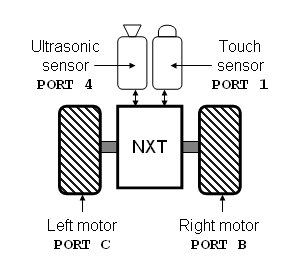
\includegraphics[height=2.4in]{figure/mindstorm/NXT_auto.png}
    \caption{Sensor/Motor configuration of the NXT Vehicle \label{fig_NXT_sensport}}
  \end{center}
\end{figure}
%%%%% END OF FIGURE %%%%%

\subsubsection{Using your touch sensor}
After you have connected your NXT to your PC, you will need to set up the sensor if you would like to include 
sensors in your NXT program. For example, if you want to add components like light sensor, ultrasonic sensor, 
and/or touch sensor, you will need to set up their connection using the \verb+setSensor()+ function. 
The \verb+setSensor()+ function will return 1 if no connection is established, so you can terminate the 
program if a sensor connection is not established. An example connection check for adding the Touch and 
Ulstrasonic sensors to the NXT vehicle is as follow:
\begin{verbatim}
ChNXT nxt;

/* Check status of NXT connection */
if (nxt.connect()){
    exit(-1);
}

/* Setup sensors and check sensor connection */
int status1=2, status2=2;

/* Save status of NXT_SENSORPORT1, and NXT_SENSORPORT4 */
status1 = nxt.setSensor(NXT_SENSORPORT1, 
            NXT_SENSORTYPE_TOUCH, NXT_SENSORMODE_BOOLEANMODE);

status2 = nxt.setSensor(NXT_SENSORPORT4,
            NXT_SENSORTYPE_ULTRASONIC, NXT_SENSORMODE_RAWMODE);
    
/* Check connection status of NXT_SENSORPORT1 */
if(status1) {
    exit(-1);
}
    
/* Check connection status of NXT_SENSORPORT4 */
if(status2) {
    exit(-1);
}
\end{verbatim}

As in previous examples, the class \verb+nxt+, is created, and the initial connection to the NXT is 
made. The next step is to initialize the NXT sensor ports to the correct types and ensure 
the sensors are working correctly. The int variables \verb+status1+ and \verb+status2+ are used to 
check the return value of the function \verb+setSensor()+.\\

A common application of touch sensors for a vehicle robot is for obstacle detection. In order to 
demonstrate the use of the touch sensor, consider the touch sensor demo in Program~\ref{prog_touchsensor.ch}.
\subsubsection*{Source Code}
%%%%%%%%%%%%%%%%%% Begin of touchsensor.ch %%%%%%%%%%%%%%%%%%%%%%%%%%%%%
\begin{comment}
\begin{Program}[H]
    {\small\verbatiminput{demos/vehicle/touchsensor.ch}}
    \caption{\texttt{touchsensor.ch} Source Code\label{prog_touchsensor.ch}}
\end{Program}
\end{comment}

\begin{Program}[H]
    {\small\verbatiminput{demos/vehicle/touchsensor.ch_part1}}
    \caption{\texttt{touchsensor.ch} Source Code\label{prog_touchsensor.ch}}
\end{Program}
\addtocounter{Program}{-1}
\begin{Program}[H]
    {\small\verbatiminput{demos/vehicle/touchsensor.ch_part2}}
    \caption{\texttt{touchsensor.ch} Source Code\label{prog_touchsensor.ch}}
\end{Program}
%%%%%%%%%%%%%%%% End of touchsensor.ch %%%%%%%%%%%%%%%%%%%%%%%%%%%%%%%%%
\subsubsection*{Checking touch sensor connection}
Program~\ref{prog_touchsensor.ch} is similar to Program~\ref{prog_forward.ch}, the only changes is 
the addition of the use of the touch sensor. Program~\ref{prog_touchsensor.ch} makes the NXT move 
forward until the touch sensor is triggered, after which it will back up and stop. One of the additions that 
is added in Program~\ref{prog_touchsensor.ch} is the initialization of the touch sensor. The fragment of 
the initialization of the touch sensor is shown below.
\begin{verbatim}
/* Set sensor types */
int status;

status = nxt.setSensor(NXT_SENSORPORT1, 
            NXT_SENSORTYPE_TOUCH, NXT_SENSORMODE_BOOLEANMODE);
if (status){
    exit(-1);
}
\end{verbatim}
In this fragment, the program use the \verb+setSensor()+ command to set the touch sensor to \verb+NXT_SENSORPORT1+. 
The connection status between the NXT and the sensor is then returned in the variable called status. Next, the 
if statement check if the connection to the sensor is good. If the variable status is equal to 1, which means
no sensor connection, the program will be exited and the rest of the codes will not be executed.
 
\subsubsection*{Using while loop}
A while loop is a common method that is used for sensor data gathering. For every iteration of the while loop, 
the program checks the data gathered by the touch sensor. After gathering the data, the program decide what to 
do with the data. A simple flow diagram of the while loop of the touch sensor demo program is shown in Figure 
\ref{fig_NXT_touchflow}\\

%%%%% START OF FIGURE %%%%%
\begin{figure}[h]
  \begin{center}
    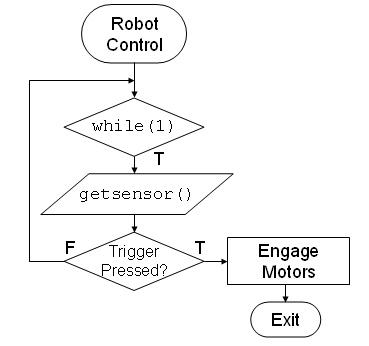
\includegraphics[height=2.4in]{figure/mindstorm/NXT_touchflow.png}
    \caption{Flow Diagram of the while loop in Program~\ref{prog_touchsensor.ch} \label{fig_NXT_touchflow}}
  \end{center}
\end{figure}
%%%%% END OF FIGURE %%%%%

\noindent
In Program~\ref{prog_touchsensor.ch}, the while loop checks for the data of the touch sensor. If 
the touch sensor is triggered, the data of the touch sensor will be set to below 500. Then the program 
will move the NXT backward and disconnect the NXT. The while loop of the touch sensor demonstration 
program is described below:
\begin{verbatim}
while(1){
    /* Get touch sensor data and save into a variable*/
    nxt.getSensor(NXT_SENSORPORT1, touchValue);
    
    /* If touch sensor is triggered */
    if (touchValue < 0){
        /* Move backward */
        nxt.setJointSpeedRatios(0, 0.25, 0.25);
        nxt.vehicleRollBackward(360);
        break;
    }
}
\end{verbatim}
In this while loop, the program uses the \verb+getSensor()+ command to get the data from \verb+NXT_SENSORPORT1+, 
which is the port for the touch sensor according to Figure \ref{fig_NXT_sensport}. Next, the program checks 
the touch sensor if it is pressed with the if statement. If the touch sensor has been triggered, the codes 
in the if statement will run. The codes inside the if statement is the same command for moving the NXT 
backward. After moving the NXT backward, the command break allows the program to exit out of the while loop.
 This while loop will never exit until the touch sensor is triggered and the break command is used.

\subsubsection{Using your ultrasonic sensor}
In order to demonstrate the use of the ultrasonic sensor, consider the ultrasonic sensor demo in 
Program~\ref{prog_ultrasonicsensor.ch}. NOTE: If your robot gets stuck, put your hands in 
front of the ultrasonic sensor to quit the loop.

\subsubsection*{Source Code}
%%%%%%%%%%%%%%%%%%%%% Begin of ultrasonicsensor.ch %%%%%%%%%%%%%%%%%%%%%%%%%%%%%%%%%%%%
\begin{comment}
\begin{Program}[H]
    {\small\verbatiminput{demos/vehicle/ultrasonicsensor.ch}}
    \caption{\texttt{ultrasonicsensor.ch} Source Code\label{prog_ultrasonicsensor.ch}}
\end{Program}
\end{comment}

\begin{Program}[H]
    {\small\verbatiminput{demos/vehicle/ultrasonicsensor.ch_part1}}
    \caption{\texttt{ultrasonicsensor.ch} Source Code\label{prog_ultrasonicsensor.ch}}
\end{Program}
\addtocounter{Program}{-1}
\begin{Program}[H]
    {\small\verbatiminput{demos/vehicle/ultrasonicsensor.ch_part2}}
    \caption{\texttt{ultrasonicsensor.ch} Source Code (Continued.)\label{prog_ultrasonicsensor.ch}}
\end{Program}
\begin{comment}
\addtocounter{Program}{-1}
\begin{Program}[H]
    {\small\verbatiminput{demos/vehicle/ultrasonicsensor.ch_part3}}
    \caption{\texttt{ultrasonicsensor.ch} Source Code (Continued.)\label{prog_ultrasonicsensor.ch}}
\end{Program}
\end{comment}
%%%%%%%%%%%%%%%%%%% End of ultrasonicsensor.ch %%%%%%%%%%%%%%%%%%%%%%%%%%%%%%%%%%%%%%

\subsubsection*{Checking touch sensor connection}
Like Program~\ref{prog_touchsensor.ch}, Program~\ref{prog_ultrasonicsensor.ch} is meant to be a 
brief demonstration of one method of using an ultrasonic sensor with a vehicle NXT. Similar to the 
initialization of the touch sensor, the initialization of the ultrasonic sensor is shown below:
\begin{verbatim}
/* Set sensor types */
int status;

status = nxt.setSensor(NXT_SENSORPORT4, 
            NXT_SENSORTYPE_ULTRASONIC, NXT_SENSORMODE_RAWMODE);

if (status){
    exit(-1);
}
\end{verbatim}

In this program fragment, the \verb+setSensor()+ command sets the ultrasonic sensor to \verb+NXT_SENSORPORT4+.
Next, it checks the return value of the sensor connection status. The program will quit if the return value 
is 1, meaning there is no connection between the sensor and the NXT.

\subsubsection*{Contents in the while loop}
In Program~\ref{prog_ultrasonicsensor.ch}, the while loop uses the ultrasonic sensor to detect distances 
between the NXT and the obstacles in front of the NXT. The ultrasonic sensor will detect distances and the 
program code reacts to the data by slowing down or speeding up. The flow diagram of the while loop of 
Program~\ref{prog_ultrasonicsensor.ch} is shown in Figure \ref{fig_NXT_ultraflow}.

%%%%% START OF FIGURE %%%%%
\begin{figure}[h]
  \begin{center}
    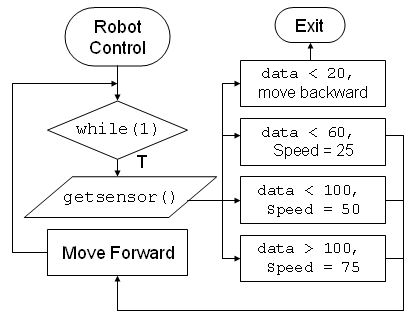
\includegraphics[height=2.4in]{figure/mindstorm/NXT_ultraflow.png}
    \caption{Flow Diagram of the while loop in Program~\ref{prog_touchsensor.ch} \label{fig_NXT_ultraflow}}
  \end{center}
\end{figure}
%%%%% END OF FIGURE %%%%%

The while loop code block for Program~\ref{prog_ultrasonicsensor.ch} is shown below:
\begin{verbatim}
/* Commands: */
while(1){
    /* Get ultrasonic sensor data */
    nxt.getSensor(NXT_SENSORPORT4, ultrasonicValue);
        
    /* If obstacle is really close */
    if (ultrasonicValue < 20){
        speedRatio = 0.25;
        /* Move backward */
        nxt.setJointSpeedRatios(0, speedRatio, speedRatio);
        nxt.vehicleRollBackward(360);
        /* Quit the while loop */
        break;
    }/* Else if the obstacle is close */
    else if(ultrasonicValue < 60){
        speedRatio = 0.25;
    }/* Else if the obstacle is not close */
    else if(ultrasonicValue < 100){
        speedRatio = 0.50;
    }/* Else if there is no obstacle in sight */
    else if(ultrasonicValue < 200){
        speedRatio = 0.75;
    }/* Sensor value larger than 200 */
    else{
        speedRatio = 0.75;
    }
    /* Move forward (constantly) */
    nxt.setJointSpeedRatios(0, speedRatio, speedRatio);
    nxt.moveJointContinuousNB(NXT_JOINT2, NXT_FORWARD);
    nxt.moveJointContinuousNB(NXT_JOINT3, NXT_FORWARD);
}
\end{verbatim}
\noindent
Similar to Program~\ref{prog_touchsensor.ch}, the while loop in Program~\ref{prog_ultrasonicsensor.ch} also gathers the 
sensor data using the \verb+getSensor()+ command to gather data from the ultrasonic sensor in 
\verb+NXT_SENSORPORT4+. Next, the if-else statement block determine what to do depending on the 
distance data from ultrasonic sensor.
\begin{itemize}
\item If the sensor value is below 20, which means the vehicle is very close to an obstacle, the program tells the
    vehicle to reverse, and then break out of the while loop.
\item If the sensor value is above 20 and below 60, which means the vehicle is close to an obstacle, the
    program set the speed raio variable to 0.25.
\item If the sensor value is above 60 and below 100, which means the vehicle is not close to an obstacle, the
    program set the speed ratio variable to 0.50.
\item If the sensor value is above 100 and below 200, which means there is nothing in front of the vehicle,
    the program set the speed ratio variable to 0.75.
\item If the sensor value is other value that is not mentioned above, the program set the speed variable to 0.75.
\end{itemize}

After the if-else statement block, the program sets the robot to move forward with velocity set at the speed variable.
Then the program returns back to the beginning of the while loop, which is to gather data from the sensor again.

%%%%%%%%%% NXT auto %%%%%%%%%%
\subsubsection{Autonomous Control Program}
In the previous sections, we thoroughly covered the manual real time control program, which allows you to 
remote control your NXT vehicle with your keyboard.
In this section, we will talk about the autonomous control program for the NXT vehicle.
In an autonomous control program, the robot, which is the NXT, must be able to move around by itself without
human commands or interventions. In order to achieve such task, the NXT must be able to detect obstacles using 
its sensors and steer away from the obstacle using its actuators.
A typical autonomous control scheme is to sense, plan, and act, which is shown in Figure \ref{fig_NXT_SPA}.
%%%%% START OF FIGURE %%%%%
\begin{figure}[h]
  \begin{center}
    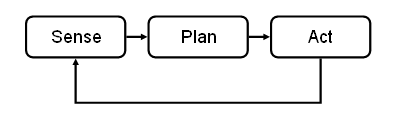
\includegraphics[height=1in]{figure/mindstorm/Senseplanact.png}
    \caption{Sense Plan Act Diagram \label{fig_NXT_SPA}}
  \end{center}
\end{figure}
%%%%% END OF FIGURE %%%%%

\begin{itemize}
\item Sense is to gather data from the robot's surrounding.
\item Plan is to plan the interaction between the robot and its surrounding using gathered data.
\item Act is to act with robot's surrounding.
\end{itemize}

The main difference between the manual RTC program and the autonomous program is the content inside the while loop.
In the manual RTC program, the codes inside the while loop scan for user's input and the robot acts on the input that
the user provided. In the autonomous program, the codes inside the while loop perform the sense-plan-act cycle similarly 
to the diagram shown in Figure \ref{fig_NXT_SPA}. Every cycle, the information is gathered from the sensor and send 
back to the computer. The computer will decide what to do depending on the sensor data. The autonomous control program 
for the NXT vehicle is described in Program~\ref{prog_vehicle_auto.ch}.

\subsubsection*{Source Code}
%%%%%%%%%%%%%%%%%%%%%%%%%%% Begin of vehicle_auto.ch %%%%%%%%%%%%%%%%%%%%%%%%%%%%%%%%%%%%%%%%
\begin{comment}
\begin{Program}[H]
    {\small\verbatiminput{demos/vehicle/vehicle_auto.ch}}
    \caption{\texttt{vehicle\_auto.ch} Source Code\label{prog_vehicle_auto.ch}}
\end{Program}
\end{comment}

\begin{Program}[H]
    {\small\verbatiminput{demos/vehicle/vehicle_auto.ch_part1}}
    \caption{\texttt{vehicle\_auto.ch} Source Code\label{prog_vehicle_auto.ch}}
\end{Program}
\addtocounter{Program}{-1}
\begin{Program}[H]
    {\small\verbatiminput{demos/vehicle/vehicle_auto.ch_part2}}
    \caption{\texttt{vehicle\_auto.ch} Source Code (Continued.)\label{prog_vehicle_auto.ch}}
\end{Program}
\addtocounter{Program}{-1}
\begin{Program}[H]
    {\small\verbatiminput{demos/vehicle/vehicle_auto.ch_part3}}
    \caption{\texttt{vehicle\_auto.ch} Source Code (Continued.)\label{prog_vehicle_auto.ch}}
\end{Program}
%%%%%%%%%%%%%%%%%%%%%%%%%%% End of vehicle_auto.ch %%%%%%%%%%%%%%%%%%%%%%%%%%%%%%%%%%%%%%%%

In Program~\ref{prog_vehicle_auto.ch}, the sensors that is used are the touch sensor and the ultra sonic sensor.
These sensors are located in the front of the vehicle so that when the vehicle encounters an obstacle, the program will
control the robot to avoid or steer away from it. A diagram of the vehicle and its sensor and actuators of the program 
is shown in Figure \ref{fig_NXT_sensport}. Please make sure your NXT vehicle are configured according to to Figure 
\ref{fig_NXT_sensport} to run Program~\ref{prog_vehicle_auto.ch}.

\subsubsection*{Exiting the while loop}
In the autonomous program, there must be codes that allow the user to quit the autonomous program.
Otherwise, the robot will roam forever until the batteries run out or until a deliberate shut down of the program.
In the beginning of the while loop, the program checks for the user's input. 
If the user's input is 'q' to quit, then the program will break out of the while loop and safely disconnects the NXT.
If the user's input is not 'q' or if the user did not input anything, the program will continue to the next section of
the while loop. The program fragment for exiting the autonomous program is shown below.

\begin{verbatim}
/* check user input 'q' to quit */
if(kbhit()){
    if (getch()=='q'){	
        printf("\nExiting.");
        break;
    }
}
\end{verbatim}

In this program fragment, an if statement is used to check if a keyboard key has been hit.
Next, if a keyboard key has been hit, another if statement checks if the input is 'q'.
If both conditions are satisfied, the break statement will break out of the while loop of the program.

\subsubsection*{Touch sensor}
The next section of the while loop uses the touch sensor to control the NXT vehicle.
When the NXT contact some obstacle in the front, the touch sensor will be triggered.
The autonomous program will notice that the touch sensor is triggered and command the 
NXT to steer away from the obstacle. The program fragment of the touch sensor is shown below.

\begin{verbatim}
/* get touch sensor. If pressed reverse and turn left */
nxt.getSensor(NXT_SENSORPORT1, touchValue);
if (touchValue <500){
    nxt.vehicleRollBackward(180);
    nxt.vehicleRotateLeft(360);
    }
\end{verbatim}

In the first line of this fragment, the NXT gathers data from \verb+NXT_SENSORPORT1+, which is the port for the touch sensor.
Next, it checks the value for the touch sensor data with an if statement.
If the value of the touch sensor data is less than 500, which means the touch sensor has been triggered, the program
will execute the obstacle avoidance commands inside the if statement.
The commands in the if statement control the NXT vehicle to reverse, then stop, and then steer left.

\subsubsection*{Ultrasonic sensor}
The next part of the while loop uses the ultrasonic sensor to control the speed of the NXT vehicle.
The ultrasonic sensor is used to detects the distance between itself to an incoming obstacle.
The distance between the ultrasonic sensor and the incoming obstacle will tell the vehicle if it should slow down or
    speed up.
For example, if the sensor senses nothing in front of the vehicle, the program will tell the vehicle to speed up; and
if the sensor senses there is an obstacle in front, the program will tell the vehicle to slow down.
The program fragment of the ultrasonic sensor is shown below.

\begin{verbatim}
/* 
 * get distance from UltraSonic sensor, 
 * set speedRatio according to distance. Turn left 
 * if really close.
 */
       
nxt.getSensor(NXT_SENSORPORT4, ultrasonicValue);
if(ultrasonicValue <10){
    nxt.vehicleRollBackward(360);
    nxt.vehicleRotateRight(180);
    speedRatio=0;
} else if (ultraValue < 30)	
    speedRatio = 0.25;
else if (ultraValue < 50)
    speedRatio = 0.50;
else if (ultraValue < 100)	
    speedRatio = 0.75;
else if (ultraValue < 200)
    speedRatio = 1;
else
    speedRatio = 0.75;
\end{verbatim}

In the first line of this fragment, the NXT gathers data from \verb+NXT_SENSORPORT4+, which is the port for the ultrasonic sensor.
Afterwards, there is a block of if-else statement to determine what speed is used for the sensor data gathered.
The if-else block changes the speed variable of the vehicle depending on the ultrasonic sensor value.
Here is the list of sensor value threshold and its commands.
\begin{itemize}
\item If the sensor value is below 10, which means the vehicle is very close to an obstacle, the program tells the
    vehicle to reverse, stop, and then steer left.
\item If the sensor value is above 10 and below 30, which means the vehicle is close to an obstacle, the
    program set the speed ratio variable to 0.25.
\item If the sensor value is above 30 and below 50, which means the vehicle sees an incoming obstacle, the
    program set the speed ratio variable to 0.50.
\item If the sensor value is above 50 and below 100, the program set the speed ratio variable to 0.75.
\item If the sensor value is above 100 and below 200, which means there is nothing in front of the vehicle,
    the program set the speed ratio variable to 1.
\item If the sensor value is other value that is not mentioned above, the program set the speed ratio variable to 0.75.
\end{itemize}


\subsubsection*{Running forward}
The autonomous program does not work if the robot is stationary.
The last portion of the while loop sets the robot to be running forward if it is not performing other tasks.
The program fragment for running forward is shown below.

\begin{verbatim}
/* Turn motors on (drive forward) */
nxt.setJointSpeedRatios(0, speedRatio, speedRatio);
nxt.moveJointContinuousNB(NXT_JOINT2, NXT_FORWARD);
nxt.moveJointContinuousNB(NXT_JOINT3, NXT_FORWARD);
\end{verbatim}

This program fragment command the vehicle to move forward continuously by setting both motors rotating positively at
the variable \verb+speedRatio+.
%%%%%%%%%% end of NXT auto %%%%%%%%%%
%%%%%%%%%%% End of Using NXT Sensors %%%%%%%%%%

\newpage
\section{Controlling Non-Vehicle NXT Robots}
Previously, the focus has been on controlling vehicle NXT designs. Ch Mindstorms NXT Control Package can 
also be used to control alternate NXT robot configurations. The following sections demonstrates Ch code 
that controls the Lego Machine NXT Robot and the Lego Bipedal Robot. These examples should give you a 
sufficient background using Ch to program the NXT to create codes for any Lego NXT creation you may make.

%%%%%%%%%%% Controlling NXT Machine %%%%%%%%%%
\subsection{Controlling NXT Machine}
%%%%% START OF FIGURE %%%%%
\begin{figure}[h]
  \begin{center}
    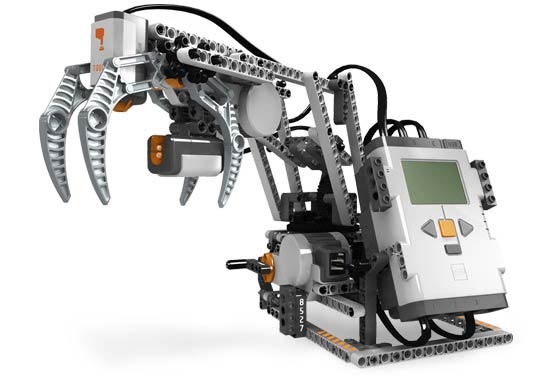
\includegraphics[height=4in]{figure/mindstorm/NXT_machine.png}
    \caption{NXT Machine\label{fig_NXT_machine}}
  \end{center}
\end{figure}
%%%%% END OF FIGURE %%%%%
\noindent
The NXT mindstorm also comes with two other forms, one of these forms is the machine form as shown in Figure
\ref{fig_NXT_machine}. In this section, the NXT machine form and the NXT machine demo program will be discussed.
Compared to the NXT vehicle, the NXT machine uses three motors to manipulate its arm and two sensors for detection.
The location and description of the components of the NXT machine is shown in Figure \ref{fig_NXT_machineMOD}.
\newpage
%%%%% START OF FIGURE %%%%%
\begin{figure}[h]
  \begin{center}
      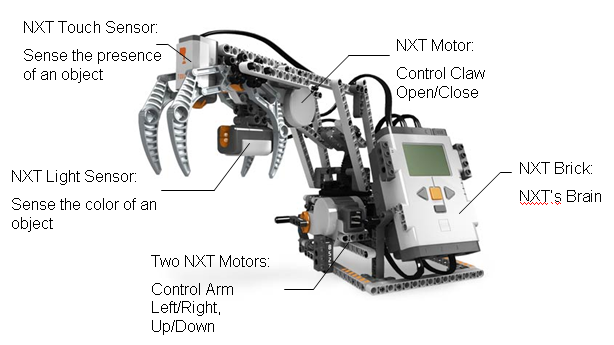
\includegraphics[height = 3in]{figure/mindstorm/NXT_machineMOD.png}
    \caption{Components of the NXT Machine\label{fig_NXT_machineMOD}}
  \end{center}
\end{figure}
%%%%% END OF FIGURE %%%%%
\noindent
As shown in Figure \ref{fig_NXT_machineMOD}, one of its motor is responsible for moving its arm left and right.
Another motor is responsible for moving its arm up and down.
The last motor is responsible for controlling its claws open and close.
There are two sensors mounted on the claw, they are the light sensor and the touch sensor.
The NXT machine uses the light sensor to sense the color of the object it is handling.
The NXT uses the touch sensor to sense if it has successfully grabbed an object.
Please use the sensor/motor port configuration shown in Figure \ref{fig_NXT_mach_port} for the
    Ch NXT machine demos programs described in later in this section.
\begin{figure}[H]
  \begin{center}
    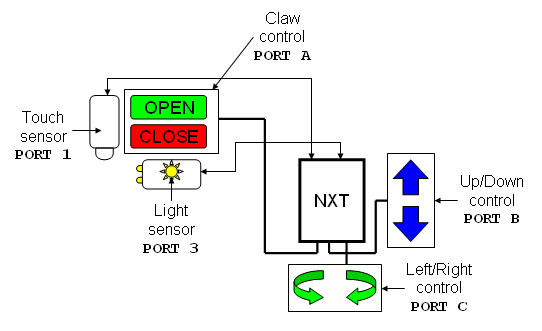
\includegraphics[height=3in]{figure/mindstorm/NXT_mach_port.png}
    \caption{Sensor/Motor configuration of the NXT Machine\label{fig_NXT_mach_port}}
  \end{center}
\end{figure}
\newpage

\subsubsection{Manual Real Time Control Program}
In this section the manual real time control for the NXT machine will be introduced and described.
The manual RTC for the NXT machine allows the user to control the NXT machine manually via the keyboard.
The user interface of the RTC program for the NXT machine is shown in Figure \ref{fig_mach_UI}
\begin{figure}[h]
  \begin{center}
    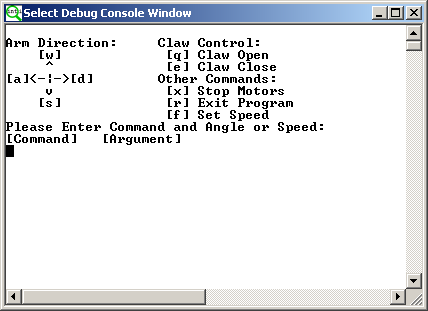
\includegraphics[height=3in]{figure/mindstorm/mach_UI.png}
    \caption{NXT vehicle RTC User Interface \label{fig_mach_UI}}
  \end{center}
\end{figure}
The user interface and the user commands for the NXT machine RTC program is a bit different compared to the
NXT vehicle RTC program. Instead of controlling the direction by pressing one key, the user will be required 
to press a key for direction or command, and then enter a number to set the angle or speed. When a specific 
key is pressed during the execution of the NXT machine RTC program, the program uses a \verb+if-else if-else+ 
statement to performs a fragment of code that send commands to the NXT to move in a direction or perform a task.
If a directional key or aset speed key has been pressed, program will ask for an user input for a number to set 
the arm to move at an angle or set the speed. If a discrete task key is pressed, like open or close claw, the 
program will not ask for an user input for a number. The list below is the list of commands and a short 
description of each commands:
\begin{itemize}
\item The key \verb+"w"+ is to control the NXT arm to move up.
\item The key \verb+"s"+ is to control the NXT arm to move down.
\item The key \verb+"a"+ is to control the NXT arm to turn left.
\item The key \verb+"d"+ is to control the NXT arm to turn right.
\item The key \verb+"q"+ is to control the NXT claw to open.
\item The key \verb+"e"+ is to control the NXT claw to close.
\item The key \verb+"x"+ is to stop the NXT motors.
\item The key \verb+"r"+ is to exit the manual RTC program.
\item The key \verb+"f"+ is to set the NXT motor speed.
\end{itemize}
The NXT machine RTC program is described in Program~\ref{prog_machine_rtc.ch}. In the rest of this section, 
we are going to explain important parts of the manual rtc program in detail.

\subsubsection*{Source Code}
%%%%%%%%%%%%%%%%%%%%%%%%%%%%%%%%% Begin of machine_rtc.ch %%%%%%%%%%%%%%%%%%%%%%%%%%%%%%%%%%%%%%%%%
\begin{comment}
\begin{Program}[H]
    {\small\verbatiminput{demos/machine/machine_rtc.ch}}
    \caption{\texttt{machine\_rtc.ch} Source Code\label{prog_machine_rtc.ch}}
\end{Program}
\end{comment}

\begin{Program}[H]
    {\small\verbatiminput{demos/machine/machine_rtc.ch_part1}}
    \caption{\texttt{machine\_rtc.ch} Source Code\label{prog_machine_rtc.ch}}
\end{Program}
\addtocounter{Program}{-1}
\begin{Program}[H]
    {\small\verbatiminput{demos/machine/machine_rtc.ch_part2}}
    \caption{\texttt{machine\_rtc.ch} Source Code (Continued.)\label{prog_machine_rtc.ch}}
\end{Program}
\addtocounter{Program}{-1}
\begin{Program}[H]
    {\small\verbatiminput{demos/machine/machine_rtc.ch_part3}}
    \caption{\texttt{machine\_rtc.ch} Source Code (Continued.)\label{prog_machine_rtc.ch}}
\end{Program}
%%%%%%%%%%%%%%%%%%%%%%%%%%%%%%%% End of machine_rtc.ch %%%%%%%%%%%%%%%%%%%%%%%%%%%%%%%%%%%%%%%%%%%

\subsubsection*{How does it work?}
The initialization and the termination of the NXT machine RTC program is very similar to the
NXT vehicle RTC program. The biggest difference between the two programs is in the while loop of the program.
In this section, we will focus on how the \texttt{while()} loop of the NXT machine RTC program work internally.

\subsubsection*{While loop}
Similar to the while loop of the NXT vehicle RTC program, the while loop of the NXT machine RTC program scans for the
variable quit to see if it is set to 1. If the 'r' key has been pressed, the variable quit will be set to 1 and the 
while loop will terminate and the machine RTC program will be terminated. In the while loop, the user will be required 
to enter different types of command. Some commands are directional command, where the user needs to enter a number 
after the command. Some commands are discrete command, where the user does not need to enter another number.
Instead of simply scanning for a key, the while loop has an additional if statement that scans for which key
was pressed. If the key is a directional key, the program ask for the user to input an angle using the \verb+scanf()+ 
command. The fragment of the while loop is shown below:

\begin{verbatim}
while (quit != 1 ) {
    printf("\nEnter command: ");
    dir = _getch();
    if ((dir == 'w') || (dir == 'a') || (dir == 's') 
            || (dir == 'd')){
        printf("  Enter angle: ");
        scanf("%d", &angle);
    }
    if(key == 'a'){
        ...
    }else if(key == 'd'){
        ...
    }else{
        ...
    }
}
\end{verbatim}

Depending on what key was pressed, the program will run a fragment of code that sends commands to the NXT using the
\verb+if-else if-else+ command.

\subsubsection*{Directional commands}
The directional movements are controlled using the 'w', 's', 'a', and 'd' keys.
In Figure \ref{fig_mach_UI}, the user interface used arrows to indicate the 
movement direction and associate each direction with a specific key.
\newline
%%% case 'a' %%%
When the key 'a' has been pressed, the \verb+if-else if-else+ statement will run the codes for the case 'a'.
The program fragment for case 'a' is shown below:
\begin{verbatim} 
if(key == 'a'){
    nxt.moveJoint(NXT_JOINT3, (int)(angle / gearratio));
}
\end{verbatim}
In case 'a', the program will run the joint \verb+NXT_JOINT3+ at velocity \verb+speedRatio+, 
and to an \verb+angle+ divided by the gear ratio that the user has entered. Basically, for case 
'a' the program will rotate the NXT machine arm left to an adjusted angle that the user has entered.\\

%%% case 'd' %%%
When the key 'd' has been pressed, the \verb+if-else if-else+ statement will run the codes for the case 'd'.
The program fragment for case 'd' is shown below:
\begin{verbatim} 
else if(key == 'd'){
    nxt.moveJoint(NXT_JOINT3, (int)(-angle / gearratio));
}
\end{verbatim}
In case 'd', the program will run the joint \verb+NXT_JOINT3+ at velocity \verb+-speedRatio+,
and to an \verb+angle+ divided by the gear ratio that the user has entered. Basically, for case 'd' 
the program will rotate the NXT machine arm right to an adjusted angle that the user has entered.\\

%%% case 'w' %%%
When the key 'w' has been pressed, the \verb+if-else if-else+ statement will run the codes for the case 'w'.
The program fragment for case 'w' is shown below:
\begin{verbatim} 
else if(key == 'w'){
    nxt.moveJoint(NXT_JOINT2, angle);
}
\end{verbatim}
In case 'w', the program will run the joint \verb+NXT_JOINT2+ at velocity \verb+speedRatio+,
and to a prescribed \verb+angle+ that the user has entered. Basically, for case 'w' the program 
will move the NXT machine arm upward to a prescribed angle that the user entered to an angle at 
a set speed ratio.\\

%%% case 's' %%%
When the key 's' has been pressed, the \verb+if-else if-else+ statement will run the codes for the case 's'.
The program fragment for case 's' is shown below:
\begin{verbatim} 
else if(key == 's'){
    nxt.moveJoint(NXT_JOINT2, -angle);
}
\end{verbatim}
In case 's', the program will run the joint \verb+NXT_JOINT2+ at velocity \verb+-speedRatio+,
and to a prescribed \verb+angle+ that the user has entered. Basically, for case 'w' the program will 
move the NXT machine arm downward to a prescribed angle that the user entered to an angle at a set speed ratio.\\

\subsubsection*{Discrete commands}
The discrete commands are commands that performs a specific task that can either be on or off.
For example, open or close the claw, turn on or off the motors, or quit the program.
For this program, the discrete commands does not require another parameter, so the user does not need to
input another number for using these commands. These commands are accessed by entering the 'q', 'e', 'x', 'r' keys.\\
\newline

%%% case 'q' %%%
When the key 'q' has been pressed, the \verb+if-else if-else+ statement will run the codes for the case 'q'.
The program fragment for case 'q' is shown below:
\begin{verbatim} 
else if(key == 'q'){
    nxt.moveJointContinuousNB(NXT_JOINT1, NXT_BACKWARD);
    delay(1);
    nxt.stopOneJoint(NXT_JOINT1);
}
\end{verbatim}
In case 'q', the program will run the joint \verb+NXT_JOINT1+ at velocity \verb+speedRatio+ for 1 seconds. Next, 
the program will hold the position of the joint at that spot, thus keeping the machine claw open. Basically, for 
case 'q' the program will open the machine claw.\\
\newline

%%% case 'e' %%%
When the key 'e' has been pressed, the \verb+if-else if-else+ statement will run the codes for the case 'e'.
The program fragment for case 'e' is shown below:
\begin{verbatim} 
else if(key == 'e'){
    nxt.moveJointContinuousNB(NXT_JOINT1, NXT_FORWARD);
    delay(1);
    nxt.stopOneJoint(NXT_JOINT1);
}
\end{verbatim}
In case 'e', the program will run the joint \verb+NXT_JOINT1+ at velocity \verb+speedRatio+ for 1 seconds. Next, 
the program will hold the position of the motor at that spot, thus keeping the machine claw close. Basically, for 
case 'e' the program will close the machine claw.

%%% case 'x' %%%
When the key 'x' has been pressed, the \verb+if-else if-else+ statement will run the codes for the case 'x'.
The program fragment for case 'x' is shown below:
\begin{verbatim} 
else if(key == 'x'){
    nxt.stopAllJoints();
}
\end{verbatim}
In case 'x', the program will stop all the motors, and turn the mode to off.\\

%%% case 'r' %%%
When the key 'r' has been pressed, the \verb+if-else if-else+ statement will run the codes for the case 'r'.
The program fragment for case 'r' is shown below:
\begin{verbatim} 
else if(key == 'r'){
    printf("\nQuit.");
    quit = 1;
}
\end{verbatim}
In case 'x', the program will print the string "Quit." and set the variable \verb+quit+ to 1.
By setting the variable \verb+quit+ to 1, the while loop will be terminated, thus quitting the program.

\subsubsection*{Speed ratio setup}
To set the speed ratio of the movement of the arm, the user can enter the key 'f' and enter the speed ratio.
The speed ratio of joints are in the range of 0 to 1. The program fragment of case 'f' is shown below:
\begin{verbatim}
else if(key == 'f'){
    printf("   Enter the speed ratio (0 to 1):");
    scanf("%lf", &speedRatio);
    printf("\nSpeed ratio set to %lf.", speedRatio);
}
\end{verbatim}

\subsubsection*{Using the sensors}
After the switch cases, the while loop will use the sensors to detect if the claw has grabbed an object or not.
If the object has been detected, the program will also try to determine the color of the object using its
light sensor In this program, the object that is grabbed is assumed to be a ball, and the color of the ball is 
assumed to be red or blue. The program fragment for this task is described below:
\begin{verbatim}
delay(0.200);
nxt.getSensor(NXT_SENSORPORT1, touchValue);
if (touchValue < 0){
    printf("    The Ball was grabbed ");
    nxt.getSensor(NXT_SENSORPORT3, colorValue);
    if (colorValue < 500){
        printf("and the color is red\n");
    }else{
        printf("and the color is blue\n");
    }
}
\end{verbatim}
In this fragment, the program will delay for 200 milliseconds and then grab the sensor value stored in
\verb+NXT_SENSORPORT1+ using the \verb+getSensor()+ command, which is the touch sensor. Afterward, the if 
statement checks if the claw has grabbed an object. If the sensor value for the touch sensor is greater 
than 500, the touch sensor is not triggered, so there is the NXT detected that there is no object in 
its claw. If the sensor value for the touch sensor is less than 500, the touch sensor is triggered and 
the NXT detected that the claw has grabbed an object. \\
\newline
When the touch sensor is trigged, the program will continue in the if statement, and the program will 
prints out that "The Ball was grabbed" in the screen and it get the sensor value stored in
\verb+NXT_SENSORPORT3+, which is the light sensor. Next, the program will determine the color of the ball 
using the light sensor value. If the light sensor value is less than 500, the NXT will detect that the 
ball that was grabbed is red and program will print out "and the color is red". If the light sensor 
value is greater than 500, the NXT will detect that the ball that was grabbed is blue and program will 
print out "and the color is blue". \\

\subsubsection{Autonomous Control Program}
In this section, the autonomous control program for the NXT machine will be introduced.
This autonomous program uses the NXT machine arm to scan it's surrounding. It performs 
this task by rotating its arm by an angle step and collect distance data with an 
ultrasonic sensor as it is rotating. At the end of the program, the collected data will be 
stored in a data file called 'output.csv', and a polar diagram of the data will be display 
for the user. The NXT machine automatic control program is described in 
Program~\ref{prog_machine_auto.ch}. In the rest of this section, we are going to explain 
important parts of the automatic control program in detail.

\subsubsection*{Source Code}
%%%%% Program~\ref{prog_machine_auto.ch} %%%%%
\begin{comment}
\begin{Program}[H]
    {\small\verbatiminput{demos/machine/machine_auto.ch}}
    \caption{\texttt{machine\_auto.ch} Source Code\label{prog_machine_auto.ch}}
\end{Program}
\end{comment}

\begin{Program}[H]
    {\small\verbatiminput{demos/machine/machine_auto.ch_part1}}
    \caption{\texttt{machine\_auto.ch} Source Code\label{prog_machine_auto.ch}}
\end{Program}
\addtocounter{Program}{-1}
\begin{Program}[H]
    {\small\verbatiminput{demos/machine/machine_auto.ch_part2}}
    \caption{\texttt{machine\_auto.ch} Source Code (Continued.)\label{prog_machine_auto.ch}}
\end{Program}
\addtocounter{Program}{-1}
\begin{Program}[H]
    {\small\verbatiminput{demos/machine/machine_auto.ch_part3}}
    \caption{\texttt{machine\_auto.ch} Source Code (Continued.)\label{prog_machine_auto.ch}}
\end{Program}
%%%%% End of Program~\ref{prog_machine_auto.ch} %%%%%%

Please use the Figure \ref{fig_NXT_machauto_port} to connect your NXT devices for the autonomous
control program.

\begin{figure}[h!]
    \begin{center}
    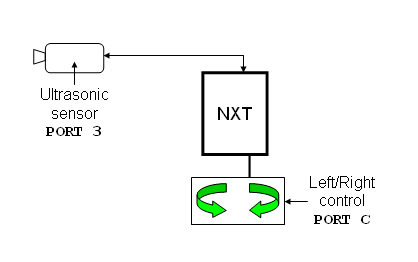
\includegraphics[height=3in]{figure/mindstorm/NXT_machauto_port.png}
    \caption{NXT vehicle RTC User Interface \label{fig_NXT_machauto_port}}
\end{center}
\end{figure}

\subsubsection*{How does it work?}
In this autonomous program, a for loop is used instead of a while loop.
The for loop will collect data, print out data, and rotate the arm at an angle step for every
loop. Some of the parameters are hardcoded in the program, for example, number of loops and angle steps,
so the user cannot change them as the autonomous program is executed. These parameters are shown in the program fragment below:

\begin{verbatim}
enum {numpoints=90};    //desired number of data points
const int anglestep=2;	//angle moved between steps
double angle[numpoints];//angle calculated from the tachometer
int distance[numpoints];//data received from the ultrasonic sensor
\end{verbatim}

The variable \verb+numpoints+ determines how many number of times the for loop will run and
the variable \verb+angles+ determines how much the arm rotates in degrees of angle.\\
Another feature this program has is the usage information printout described in the program fragment below.
\begin{verbatim}
printf("\n%d Data points will be collected with a"
        "step size of %d.",numpoints,anglestep);

printf("\nPlease ensure that the arm can rotate"
        "%d degrees from its current position.",(numpoints*anglestep));

printf("\nPress any key to continue. Press q at any time to quit.");

if(getch()=='q'){
    printf("\nQuitting program.");
    delay(1.500);
    exit(-1);
}
\end{verbatim}

In this program fragment, the program will print out how many data point will be collected
with the angle step size. Next, it will calculate and print out the full rotation angle of 
the robot arm and ask the user to ensure that the arm can rotate that amount of angle.
Lastly, the program asks the user to continue or quit the program.

\subsubsection*{For loop}
The for loop is the main part of the autonomous program for the NXT machine.
The for loop uses a series of if-else statements to perform data collection and arm movement.
There are three sections for this for loop. The first section is to collect, store, and print 
ultrasonic data and angle rotation data. The second section scans for user input to see if the 
user has pressed 'q' to quit the program. The last section is to rotate the arm by an angle step.
The program fragment below is the for loop for the autonomous program for the NXT machine.

\begin{verbatim}
for(i=0;i<numpoints;i++){
    /* get sensor data, if success print data, else print error*/
    if((nxt.getSensor(NXT_SENSORPORT4, ultraValue))){
        distance[i]= ultraValue;
        if (nxt.getJointAngle(NXT_SENSORPORT3, angle[i] == 0)){
            printf("\nSample: %d,  distance: %d,  Angle: %lf",
                        i, distance[i],angle[i]);
        }
    }else	
        printf("\nError!");

    /* check if q was pressed and if so exit program */
    if (!_kbhit){
        if(getch()=='q'){
            printf("\nQuitting program.");
            break;
        }
    }		

    /* rotate arm by anglestep (rotate motor 
       anglestep/gear ratio)*/
    nxt.moveJoint(NXT_JOINT3, (anglestep/gearratio));
    delay(1);
}
\end{verbatim}

The first section of the for loop begins at the line after the first comment and ends at the line
before the second comment. The first section begins by getting the ultrasonic sensor data and store 
it in an array. If the program is able to retrieve the data, the program will also get the data from 
the tachometer and convert it to angle. The calculated angle will be stored in another array.
Next, the program will print the sample number, distance detected by ultrasonic sensor, and angle
rotated by the motor. If the program is unable to retrieve the data, the program will print error.\\ 
\newline
The second section of the for loop begins at the line after the second comment and ends at the line
before the third comment. In this section, the program checks if a key has been hit by the user, if 
no key has been hit, this section is skipped. If a key has been hit and it happened to be the 'q' 
key, the program will print 'Quitting program' and the program will be aborted.\\
\newline
The third section of the for loop begins at the line after the third comment and ends at the end of
the for loop. In this section, the program controls the motor to rotate at a given angle using the 
\verb+moveJoint()+ command. Lastly, the program freezes for 1 second by using the \verb+delay()+ command.

\subsubsection*{Plotting data}
In addition to creating and storing a data file, the program also plots a polar diagram for
the user to visualize the data. The program fragment below are the commands for plotting the 
data in a polar diagram.

\begin{verbatim}
//plot data in CH using a polar graph
plot.polarPlot(PLOT_ANGLE_DEG);
plot.data2DCurve(angle, distance, numpoints);
plot.sizeRatio(1);
plot.grid(PLOT_ON); 
plot.plotting();
\end{verbatim}

In this fragment, the program uses the CPlot class commands to do its plotting.
First, the program use the function \verb+polarPlot()+ to set the plot to polar and degrees in angle.
Next, the program use the function \verb+data2DCurve()+ to insert the collected data onto the polar plot.
Afterward, the program uses the function \verb+sizeRatio()+ function and \verb+grid()+ command to
correct the size of the plot and to add grid to the plot. Finally, the program creates the plot by using 
the function \verb+plotting()+.
%%%%%%%%%%% End of Controlling Your NXT Machine %%%%%%%%%%

\clearpage
\newpage
%%%%%%%%%%% Controlling NXT Humanoid %%%%%%%%%%
\subsection{Controlling NXT Humanoid}
%%%%% START OF FIGURE %%%%%
\begin{figure}[ht]
  \begin{center}
    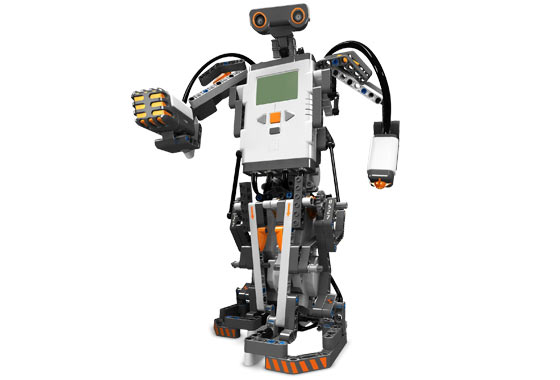
\includegraphics[height=2.5in]{figure/mindstorm/NXT_humanoid.png}
    \caption{NXT Humanoid \label{fig_NXT_humanoid}}
  \end{center}
\end{figure}

\noindent
The third form of the NXT mindstorm is the humanoid form as shown in Figure \ref{fig_NXT_humanoid}
The NXT humanoid uses two of its motors to perform the walking motion. Also, the NXT humanoid uses 
its last motor to control the rotation of its head. The NXT humanoid is equipped with four sensors, 
a sound sensor on its right hand, a touch sensor on its left hand, a light sensor in the back, and 
an ultrasonic sensor on its head. In the next section, the real time control program for the NXT 
humanoid will be discussed. Please configure your NXT sensors and motors according to Figure 
\ref{fig_NXT_human_port}

\begin{figure}[ht]
  \begin{center}
    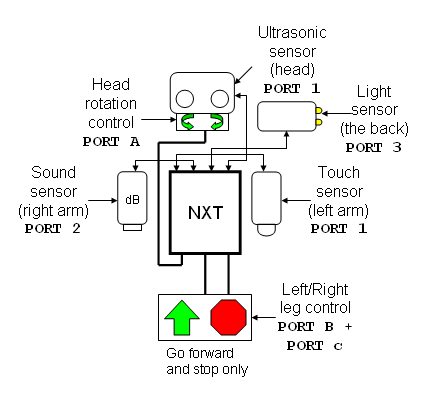
\includegraphics[height=2.5in]{figure/mindstorm/NXT_human_port.png}
    \caption{Sensor/Motor configuration of the NXT Humanoid\label{fig_NXT_human_port}}
  \end{center}
\end{figure}

\newpage
\subsubsection{Manual Real Time Control Program}
The real time control program of the NXT humanoid is similar to the real time control program of the NXT vehicle.
The RTC program of the NXT humanoid allows the user to control the robot's leg movement and head rotation using the
keyboard. In addition, the RTC program allow the user to print out data that has been collected by the NXT sensor.
Figure \ref{fig_human_UI} shows the user interface of the NXT humanoid.

\begin{figure}[ht]
  \begin{center}
    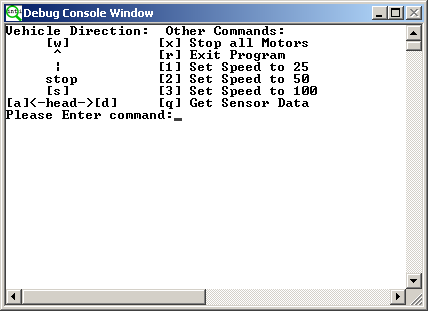
\includegraphics[height=3in]{figure/mindstorm/human_UI.png}
    \caption{NXT Humanoid RTC User Interface \label{fig_human_UI}}
  \end{center}
\end{figure}

The list below is the list of commands:
\begin{itemize}
\item The key \verb+"w"+ is to control the NXT humanoid to walk forward.
\item The key \verb+"s"+ is to control the NXT humanoid to stop.
\item The key \verb+"a"+ is to control the NXT humanoid head to turn left.
\item The key \verb+"d"+ is to control the NXT humanoid head to turn right.
\item The key \verb+"q"+ is to print out sensor data.
\item The key \verb+"x"+ is to stop all of the NXT motors.
\item The key \verb+"r"+ is to exit the RTC program.
\item The number key is to set the NXT motor speed.
\end{itemize}

The NXT humanoid real time control program is described in Program~\ref{prog_humanoid_rtc.ch}. 
In the rest of this section, we are going to explain important parts of the manual RTC program in detail.

\subsubsection*{Source Code}
%%%%% Program~\ref{prog_humanoid_rtc.ch} %%%%%
\begin{comment}
\begin{Program}[H]
    {\small\verbatiminput{demos/humanoid/humanoid_rtc.ch}}
    \caption{\texttt{humanoid\_rtc.ch} Source Code\label{prog_humanoid_rtc.ch}}
\end{Program}
\end{comment}

\begin{Program}[H]
    {\small\verbatiminput{demos/humanoid/humanoid_rtc.ch_part1}}
    \caption{\texttt{humanoid\_rtc.ch} Source Code\label{prog_humanoid_rtc.ch}}
\end{Program}
\addtocounter{Program}{-1}
\begin{Program}[H]
    {\small\verbatiminput{demos/humanoid/humanoid_rtc.ch_part2}}
    \caption{\texttt{humanoid\_rtc.ch} Source Code (Continued.)\label{prog_humanoid_rtc.ch}}
\end{Program}
\addtocounter{Program}{-1}
\begin{Program}[H]
    {\small\verbatiminput{demos/humanoid/humanoid_rtc.ch_part3}}
    \caption{\texttt{humanoid\_rtc.ch} Source Code (Continued.)\label{prog_humanoid_rtc.ch}}
\end{Program}
%%%%% End of Program~\ref{prog_humanoid_rtc.ch} %%%%%%
%%%%% END OF FIGURE %%%%%

\subsubsection*{How does it work?}
The the main difference between the RTC program for the NXT humanoid and the NXT vehicle is the content 
in the switch cases. Other than the switch cases, the while loop of the RTC program is the same as the 
previous RTC program. When the key 'r' has been pressed, the \verb+if-else if-else+ statement will run the codes 
for the case 'r'. In the case 'r', the variable quit will be to 1, which will allow the program to exit 
the while loop, thus quitting the program.\\
\newline

%%% case 'w' %%%
When the key 'w' has been pressed, the \verb+if-else if-else+ statement will run the codes for the case 'w'.
The program fragment for case 'w' is shown below:

\begin{verbatim} 
if(key == 'w')//up
    nxt.moveJointContinuousNB(NXT_JOINT2, NXT_FORWARD);
    nxt.moveJointContinuousNB(NXT_JOINT3, NXT_FORWARD);
    movemode='w';
    break;
\end{verbatim}
In case 'w', the program will run joints \verb+NXT_JOINT2+ and \verb+NXT_JOINT3+ at velocity \verb+speedRatio+. 
Basically, for case 'w' the program will control the NXT humanoid to walk forward at a speed ratio.\\
\newline

%%% case 's' %%%
When the key 's' has been pressed, the \verb+if-else if-else+ statement will run the codes for the case 's'.
The program fragment for case 's' is shown below:

\begin{verbatim} 
else if(key == 's'){//down
    nxt.stopOneJoint(NXT_JOINT2);
    nxt.stopOneJoint(NXT_JOINT3);
    movemode='s';
}
\end{verbatim}
In case 's', the program will stop joints \verb+NXT_JOINT2+ and \verb+NXT_JOINT3+ and turn them to off.
Basically, for case 's' the program will stop the NXT humanoid from walking forward.\\
\newline

%%% case 'a' %%%
When the key 'a' has been pressed, the \verb+if-else if-else+ statement will run the codes for the case 'a'.
The program fragment for case 'a' is shown below:
\begin{verbatim} 
else if(key == 'a'){//left
    nxt.setJointSpeedRatio(NXT_JOINT1, 0.3);
    nxt.moveJointContinuousNB(NXT_JOINT1, NXT_BACKWARD);
}
\end{verbatim}
In case 'a', the program will run joints \verb+NXT_JOINT1+ at a speed ratio of 0.3.
Basically, for case 'a' the program will rotate the NXT humanoid head left.\\
\newline

%%% case 'd' %%%
When the key 'd' has been pressed, the \verb+if-else if-else+ statement will run the codes for the case 'd'.
The program fragment for case 'd' is shown below:
\begin{verbatim} 
else if(key == 'd'){//right
    nxt.setJointSpeedRatio(NXT_JOINT1, 0.3);
    nxt.moveJointContinuousNB(NXT_JOINT1, NXT_FORWARD);
}
\end{verbatim}

In case 'd', the program will run the joint \verb+NXT_JOINT1+ at a speed ratio of 0.3.
Basically, for case 'd' the program will rotate the NXT humanoid head right.\\
\newline

%%% case 'q' %%%
When the key 'q' has been pressed, the \verb+if-else if-else+ statement will run the codes for the case 'q'.
The program fragment for case 'q' is shown below:
\begin{verbatim} 
else if(key == 'q'){//print sensor
    printSensor();
}
\end{verbatim}
In case 'q', the program will run the function \verb+printSensor()+, which will get sensor data from each data and
print these data out for the user. The details of the \verb+printSensor()+ function will be discussed later in this 
section.\\
\newline

%%% case 'x' %%%
When the key 'x' has been pressed, the \verb+if-else if-else+ statement will run the codes for the case 'x'.
The program fragment for case 'x' is shown below:
\begin{verbatim} 
else if(key == 'x'){//stop
    nxt.stopOneJoint(NXT_JOINT2);
    nxt.stopOneJoint(NXT_JOINT3);
    movemode='x';
}
\end{verbatim}
In case 'x', the program will stop all the motors connected to the NXT and set them to off idle mode.

\subsubsection*{Printing sensor data}
The function definition for the function \verb+printSensor+ is shown in the program fragment below:

\begin{verbatim}
int printSensor(ChNXT *nxt){
    int touchValue=0;
    int ultraValue=0;
    int soundValue=0;
    int lightValue=0;

    nxt->getSensor(NXT_SENSORPORT1, touchValue);
    nxt->getSensor(NXT_SENSORPORT2, ultraValue);
    nxt->getSensor(NXT_SENSORPORT3, soundValue);
    nxt->getSensor(NXT_SENSORPORT4, lightValue);

    if (touch < 0)
        printf("\n\n\nThe touch sensor has been activated.\n", touchValue);
    else
        printf("\nThe touch sensor has not been activated.\n");

    printf("The distance reported by the ultrasonic sensor is %d.\n",
                    ultraValue);
    /*
    if (light<500)  
        printf("\nThe touch sensor has been activated\n");
    else    
        printf("\nThe touch sensor has been activated\n");
    */
    printf("The light level is %d.\n",lightValue);
    printf("The Sound level is %dDb\n\n\n",soundValue);
    
    //GUI display
    printf("Vehicle Direction:  Other Commands:");
    printf("\n     [w]           [x] Stop all Motors");
    printf("\n      ^            [r] Exit Program");
    printf("\n      |            [1] Set Speed Ratio to 0.25");
    printf("\n     stop          [2] Set Speed Ratio to 0.50");
    printf("\n     [s]           [3] Set Speed Ratio to 0.75");
    printf("\n[a]<-head->[d]     [q] Get Sensor Data\n");
    printf("Please Enter command:");
    return 0;
}
\end{verbatim}

In the beginning of this function, the program get sensor data from each sensor and store them in its corresponding
variable. Next, if else statements are used to print the correct statement if the sensor is triggered or not.
For example, if the touch sensor is triggered, the sensor data retrieved is below 500, then the program will
print 'The touch sensor has been activated'. Next, the program will print out the distance collected by the 
ultrasonic sensor, then the light sensor and lastly the sound sensor. Finally, the function prints the user 
interface again for the user to read.
%%%%%%%%%%% End of Controlling Your NXT Humanoid %%%%%%%%%%
%% appendix %%
\newpage
\appendix
%%%%%%%%%% APPENDIX %%%%%%%%%%
\section{\label{sec:chnxt_api}ChNXT Class API}
The header file nxt.h defines all the data types, macros and 
function prototypes for th Lego Mindstorms NXT API library. 
The header file declares a class called ChNXT which contains
member functions which may be used to control the Lego
Minstorms NXT.\\
%% DATA TYPE %%
\subsection{\label{sec:datatypes}Data Types Used in ChNXT Class}
The data types defined in the header file \texttt{nxt.h} are 
described in this appendix. These data types are used by the NXT 
library to represent certain values, such as joint id's and motor 
directions.\\

\noindent
\begin{tabular}{p{3.5cm}p{12cm}} 
\hline 
Data Type& Description \\
\hline 
\texttt{nxtJointId\_t} & An enumerated value that indicates a 
nxt joints. \\
\texttt{nxtJointState\_t} & The current state of a nxt joint. \\
\texttt{nxtSensorId\_t} & An enumerate value that indicates a 
nxt's sensors. \\
\texttt{nxtSensorType\_t} & An enumerate value that indicates 
the type of a sensor of a nxt.\\
\texttt{nxtSensorMode\_t} & An enumerate value that indicates 
the mode of a sensor for getting value. \\
\hline
\end{tabular}

\subsubsection{\label{sec:nxtJointId_t}\texttt{nxtJointId\_t}}
This datatype is an enumerated type used to identify a joint on 
the Lego Mindstorms NXT. Valid values for this type are:
\begin{verbatim}
typedef enum nxt_joints_e {
  NXT_JOINT1 = 0,
  NXT_JOINT2 = 1,
  NXT_JOINT3 = 2,
} nxtJointId_t;
\end{verbatim}
\index{nxt\_joints\_t}

\index{NXT\_JOINT1}
\index{NXT\_JOINT2}
\index{NXT\_JOINT3}

\noindent
\begin{tabular}{p{3.5cm}p{12cm}} \hline 
Value & Description \\
\hline 
\texttt{NXT\_JOINT1} & PortA on the Lego Mindstorms NXT. \\
\texttt{NXT\_JOINT2} & PortB on the Lego Mindstorms NXT. \\
\texttt{NXT\_JOINT3} & PortC on the Lego Mindstorms NXT. \\
\hline
\end{tabular}

\subsubsection{\label{sec:nxtJointState_t}\texttt{nxtJointState\_t}}
This datatype is an enumerated type used to designate the current 
movement state of a joint. The values may be retrieved from the 
robot with the \texttt{getJointState()} function and may be set 
with the \texttt{moveContinuous()} family of functions. Valid values are:

\begin{verbatim}
typedef enum nxt_joint_state_e {
    NXT_FORWARD   = 1,
    NXT_BACKWARD  = -1,
} nxtJointState_t;
\end{verbatim}

\index{nxtJointState\_t}

\index{NXT\_FORWARD}
\index{NXT\_BACKWARD}

\noindent
\begin{tabular}{p{3.5cm}p{12cm}} \hline 
Value & Description \\
\hline
\texttt{NXT\_FORWARD} & This value indicates that the joint is currently moving forward.  \\
\texttt{NXT\_BACKWARD}& This value indicates that the joint is currently moving backward. \\
\hline
\end{tabular}
\\

\subsubsection{\label{sec:nxtSensorPort_t}\texttt{nxtSensorPort\_t}}
This datatype is an enumerated type used to identify a sensor on 
the Lego Mindstorms NXT. Valid values for this type are:

\begin{verbatim}
typedef enum nxt_sensors_e{
    NXT_SENSORPORT1 = 0,
    NXT_SENSORPORT2 = 1,
    NXT_SENSORPORT3 = 2,
    NXT_SENSORPORT4 = 3
} nxtSensorId_t;
\end{verbatim}
\index{nxtSensorId\_t}

\index{NXT\_SENSORPORT1}
\index{NXT\_SENSORPORT2}
\index{NXT\_SENSORPORT3}
\index{NXT\_SENSORPORT4}

\noindent
\begin{tabular}{p{3.5cm}p{12cm}} \hline
Value &       Description\\
\hline
\texttt{NXT\_SENSORPORT1}&Select sensor input PORT 1 on the NXT.\\
\texttt{NXT\_SENSORPORT2}&Select sensor input PORT 2 on the NXT.\\
\texttt{NXT\_SENSORPORT3}&Select sensor input PORT 3 on the NXT.\\
\texttt{NXT\_SENSORPORT4}&Select sensor input PORT 4 on the NXT.\\
\hline
\end{tabular}

\subsubsection{\label{sec:nxtSensorType_t}\texttt{nxtSensorType\_t}}
This data type is used to identify the type of a sensor for the
Lego Mindstorms NXT. Valid values for this type are:

\begin{verbatim}
typedef enum nxt_sensor_type_e{
    NXT_SENSORTYPE_TOUCH           = 0x01,
    NXT_SENSORTYPE_TEMPERATURE     = 0x02,
    NXT_SENSORTYPE_LIGHT_ACTIVE    = 0x05,
    NXT_SENSORTYPE_LIGHT_INACTIVE  = 0x06,
    NXT_SENSORTYPE_SOUND_DB        = 0x07,
    NXT_SENSORTYPE_SOUND_DBA       = 0x08,
    NXT_SENSORTYPE_LOWSPEED        = 0x0A,
    NXT_SENSORTYPE_ULTRASONIC      = 0x0B // LOWSPEED_9V
} nxtSensorType_t;
\end{verbatim}

\index{nxtSensorType\_t}

\index{NXT\_SENSORTYPE\_TOUCH}
\index{NXT\_SENSORTYPE\_TEMPERATURE}
\index{NXT\_SENSORTYPE\_LIGHT\_ACTIVE}
\index{NXT\_SENSORTYPE\_LIGHT\_INACTIVE}
\index{NXT\_SENSORTYPE\_SOUND\_DB}
\index{NXT\_SENSORTYPE\_SOUND\_DBA}
\index{NXT\_SENSORTYPE\_ULTRASONIC}

\noindent
\begin{tabular}{p{5.5cm}p{10cm}} \hline
Value &       Description\\
\hline
\texttt{NXT\_SENSORTYPE\_TOUCH}          &Set to Touch sensor.\\
\texttt{NXT\_SENSORTYPE\_TEMPERATURE}   &Set to Temperature Sensor.\\
\texttt{NXT\_SENSORTYPE\_LIGHT\_ACTIVE} &Set to Light Sensor in active mode(LED on).\\
\texttt{NXT\_SENSORTYPE\_LIGHT\_INACTIVE}&Set to Light Sensor in inactive mode(LED off).\\
\texttt{NXT\_SENSORTYPE\_SOUND\_DB}    &Set to Sound Sensor in dB.\\
\texttt{NXT\_SENSORTYPE\_SOUND\_DBA}   &Set to Sound Sensor in dBa.\\
\texttt{NXT\_SENSORTYPE\_LOWSPEED}     &Set to ISP type sensor.\\
\texttt{NXT\_SENSORTYPE\_ULTRASONIC}   &Set to Ultrasonic Sensor.\\
\hline
\end{tabular}

\subsubsection{\label{sec:nxtSensorMode_t}\texttt{nxtSensorMode\_t}}
This data type is used to identify the mode for a sensor to get value for the Lego Mindstorms NXT. Valid values for this type are:

\begin{verbatim}
typedef enum nxt_sensor_mode_e{
    NXT_SENSORMODE_RAWMODE         = 0x00,
    NXT_SENSORMODE_BOOLEANMODE     = 0x20
} nxtSensorMode_t;
\end{verbatim}
\index{nxtSensorMode\_t}

\index{NXT\_SENSORMODE\_RAWMODE}
\index{NXT\_SENSORMODE\_BOOLEANMODE}

\noindent
\begin{tabular}{p{5.5cm}p{10cm}} \hline
Value & Description\\
\hline
\texttt{NXT\_SENSORMODE\_RAWMODE}	    &Get sensor value as raw mode.\\	 
\texttt{NXT\_SENSORMODE\_BOOLEANMODE}  &Get sensor value as boolean mode.\\
\hline
\end{tabular}
%%%%%%%%%% End of Data Types %%%%%%%%%%

%%%%%%%%%%%%%%%%%%%%%%%%%%% ChNXT Class API %%%%%%%%%%%%%%%%%%%%%%%%%%%%

%%%%%%%%%%%%%%%% the table of communication functions %%%%%%%%%%%%
\subsection{ChNXT Class API Overview}
\begin{table}[!h]
\caption{Functions for Communication}

\begin{tabular}{ p{6cm}p{10cm}}\hline
Function & Description\\
\hline
\texttt{connect()}&Connects to the Mindstorms NXT using bluetooth 
(Read bluetooth address from the configuration file automaticly).\\
\texttt{connectWithAddress()}&Connects to the Mindstorms NXT via 
bluetooth (Read bluetooth address from users' input).\\
\texttt{disconnect()}  &Disconnects from the Mindstorms NXT.\\
\hline
\end{tabular}
\end{table}

% the table for the checking functions %
\begin{table}[!h]
\caption{Functions for Checking Status}
\begin{tabular}{ p{6cm}p{10cm}}\hline
Function & Description\\
\hline
\texttt{isConnected()}    &Check the connection to a robot.\\
\texttt{isMoving()}       &Check if any joints are currently in motion.\\
\hline
\end{tabular}
\end{table}

% the table for the sensors' functions %
\begin{table}[!h]
\caption{Functions for Sensors}
\begin{tabular}{ p{6cm}p{10cm}}\hline
Function & Description\\
\hline
\texttt{setSensor()}       &Setup the sensors to collect data from the environment.\\
\texttt{getSensor()}       &Get the data collected by the sensors from the NXT.\\
\hline
\end{tabular}
\end{table}

%%%%%%%%%%%%%%% functions for joints %%%%%%%%%%%%%%
\begin{table}[!h]
\caption{Functions for Joints}
\begin{tabular}{ p{6cm}p{10cm} }\hline
Functions & Description\\
\hline
\texttt{setJointZero()}         &Reset the tachometer to zero for a single joint.\\
\texttt{setJointZeros()}        &Reset the tachometer to zero for all joints.\\
\texttt{setJointSpeedRatio()}   &Set up a single joint speed.\\
\texttt{setJointSpeedRatios()}  &Set up all joints' speed.\\
\texttt{moveJointContinuousNB()}&Make a single joint move continuously.\\
\texttt{moveJoint()}            &Make a single joint move a user-specified angle.\\
\texttt{moveJointNB()}          &Identical to \texttt{moveJoint()} but non-blocking.\\
\texttt{moveJointTo()}          &Make a single joint move to an absolute angle.\\
\texttt{moveJointToNB()}        &Identical to \texttt{moveJointTo()} but non-blocking.\\
\texttt{move()}                 &Make all joints move a user-specified angles.\\
\texttt{moveNB()}               &Identical to \texttt{move()} but non-blocking.\\
\texttt{moveTo()}               &Make all joints move to absolute angles.\\
\texttt{moveToNB()}             &Identical to \texttt{moveTo()} but non-blocking.\\
\texttt{moveToZero()}           &Make all joints move to absolute zero positions.\\
\texttt{moveToZeroNB()}         &Identical to \texttt{moveToZero()} but non-blocking.\\
\texttt{moveContinuousNB()}     &Make all joints move continuously.\\
\texttt{moveContinuousTime()}   &Make all joints move continuously for a certain amount of time.\\
\texttt{moveWait()}             &Wait untill all motors have stopped moving.\\
\texttt{getJointAngle()}        &Get tachometer counts from NXT.\\
\texttt{getJointSpeedRatio()}   &Get a motor's speed ratio from NXT.\\
\texttt{getJointSpeedRatios()}  &Get all motors' speed ratios from NXT.\\
\texttt{stopOneJoint()}         &Make a single joint stop moving.\\
\texttt{stopTwoJoints()}        &Make two joints stop moving.\\
\texttt{stopAllJoints()}        &Make all joints stop moving.\\
\hline
\end{tabular}
\end{table}

% the functions for vehicle configuration %
\begin{table}[!h]
\caption{Functions for the Vehicle Configuration}
\begin{tabular}{ p{6cm}p{10cm} }\hline
Functions & Description\\
\hline
\texttt{vehicleRollForward()}      &Moves the NXT vehicle forward.\\
\texttt{vehicleRollForwardNB()}    &Identical to \texttt{vehicleRollForward()}, but non-blocking.\\
\texttt{vehicleRollBackward()}     &Moves the NXT vehicle backward.\\
\texttt{vehicleRollBackwardNB()}   &Identical to \texttt{vehicleRollBackward()}, but non-blocking.\\
\texttt{vehicleRotateLeft()}       &Rotates the NXT vehicle left.\\
\texttt{vehicleRotateLeftNB()}     &Identical to \texttt{vehicleRotateLeft()}, but non-blocking.\\
\texttt{vehicleRotateRight()}      &Rotates the NXT vehicle right.\\
\texttt{vehicleRotateRightNB()}    &Identical to \texttt{vehicleRotateRight()}, but non-blocking.\\
\texttt{vehicleMotionWait()}       &Wait until vehicle stop moving.\\
\hline
\end{tabular}
\end{table}

\clearpage
\newpage
% functions details %
\subsection{ChNXT Class API Details}
\noindent
\vspace{5pt}
\rule{4.5in}{0.015in}\\
\noindent
{\LARGE \texttt{ChNXT::connect()} \index{ChNXT::connect()}}\\

\addcontentsline{toc}{subsection}{connect()}

\noindent
{\bf Synopsis}
%\vspace{-8pt}
\begin{lstlisting}
#include <nxt.h>
int ChNXT::connect();
\end{lstlisting}

\noindent
{\bf Purpose}\\
Connect to a Mindstorms NXT via Bluetooth.\\

\noindent
{\bf Return Value}\\
The function returns 0 on success, and non-zero otherwise.\\

\noindent
{\bf Parameters}\\
None.\\

\noindent
{\bf Description}\\
This function is used to connect to a Mindstorms NXT via Bluetooth. The Bluetooth address is gotten from the configuration file.\\

\noindent
{\bf Example}
\begin{lstlisting}
#include <nxt.h> 

ChNXT nxt;
if (nxt.connect()){
    printf("Connection to NXT has failed.");
    exit(0);
}
\end{lstlisting}

\noindent
{\bf See Also}\\
\texttt{connectWithAddress()}, \texttt{disconect()}\\
%%%%% END OF ChNXT::connect %%%%%

\noindent
\vspace{5pt}
\rule{4.5in}{0.015in}\\
\noindent
{\LARGE \texttt{ChNXT::connectWithAddress()} \index{ChNXT::connectWithAddress()}}\\

\addcontentsline{toc}{subsection}{connectWithAddress()}

\noindent
{\bf Synopsis}
\vspace{-8pt}
\begin{verbatim}
#include <nxt.h>
int ChNXT::connectWithAddress(char usr_addr[18]);
\end{verbatim}

\noindent
{\bf Purpose}\\
Connect to a Mindstorms NXT via Bluetooth.\\

\noindent
{\bf Return Value}\\
The function returns 0 on success, and non-zero otherwise.\\

\noindent
{\bf Parameters}\\
\vspace{-0.1in}
\begin{description}
\item
\begin{tabular}{p{20mm}p{135mm}}
\texttt{usr\_address} & The Bluetooth address of the Mindstorm NXT.
\end{tabular}
\end{description}

\noindent
{\bf Description}\\
This function is used to connect to a Mindstorms NXT via Bluetooth. The Bluetooth address is gotten from the configuration file.\\

\noindent
{\bf Example}
\begin{verbatim}
#include <nxt.h> 

ChNXT nxt;
if (nxt.connectWithAddress("00:16:53:12:e7:80")){
    printf("Connection to NXT has failed.");
    exit(0);
}
\end{verbatim}

\noindent
{\bf See Also}\\
\texttt{connect()}, \texttt{disconnect()}\\
%%%%% END OF ChNXT::connectWithAddress %%%%%

\noindent
\vspace{5pt}
\rule{4.5in}{0.015in}\\
\noindent
{\LARGE \texttt{ChNXT::disconnect()} \index{ChNXT::disconnect()}}\\

\addcontentsline{toc}{subsection}{disconnect()}

\noindent
{\bf Synopsis}
\begin{lstlisting}
#include <nxt.h>
int ChNXT::disconnect();
\end{lstlisting}

\noindent
{\bf Purpose}\\
Disconnect from a Lego mindstorms NXT.\\

\noindent
{\bf Return Value}\\
The function returns 0 on success and non-zero otherwise.\\

\noindent
{\bf Parameters}\\
None.\\

\noindent
{\bf Description}\\
This function is used to disconnect from a connected Mindstorms NXT. A call to this function is not necessary before the terminationof a program. It is only neccessary if another connection will be established within the same program at a later time.\\

\noindent
{\bf Example}
\begin{lstlisting}
#include <nxt.h> 

ChNXT nxt;
if (nxt.connectWithAddress("00:16:53:12:e7:80")){
    printf("Connection to NXT has failed.");
    exit(0);
}
    
nxt.disconnect();
\end{lstlisting}

\noindent
{\bf See Also}\\
\texttt{connect()}, \texttt{connectWithAddress}\\
%%%%% END OF ChNXT::connect %%%%%

%\newpage
\noindent
\vspace{5pt}
\rule{4.5in}{0.015in}\\
\noindent
{\LARGE \texttt{ChNXT::getJointAngle()}\index{ChNXT::getJointAngle()}}\\
%\phantomsection
\addcontentsline{toc}{subsection}{getJointAngle()}

\noindent
{\bf Synopsis}
\begin{lstlisting}
#include <nxt.h>
int ChNXT::getJointAngle(nxtJointId_t id, double &angle);
\end{lstlisting}

\noindent
{\bf Purpose}\\
Retrieve a robot joint's current angle.\\

\noindent
{\bf Return Value}\\
The function returns 0 on success and non-zero otherwise.\\

\noindent
{\bf Parameters}\\
\vspace{-0.1in}
\begin{description}
\item               
\begin{tabular}{p{15 mm}p{145 mm}}
\texttt{id} & The joint number. This is an enumerated type 
discussed in Section \ref{sec:nxtJointId_t} on page
\pageref{sec:nxtJointId_t}.\\
\texttt{angle} & A variable to store the current angle of the robot
motor. The contents of this variable will be overwritten with a value that
represents the motor's angle in degrees.  \\
\end{tabular}
\end{description}

\noindent
{\bf Description}\\
This function gets the current motor angle of a NXT's motor. The
angle returned is in units of degrees and is accurate to roughly $\pm1$
degrees. The function \texttt{getJointAngle()} always returns an angle 
from 0 to $\infty$ degrees.\\

\noindent
{\bf Example}
\begin{lstlisting}
#include <nxt.h>

ChNXT nxt;
double angle;

nxt.connect();

nxt.getJointAngle(NXT_JOINTA, angle);

printf("The angle of jointA is: %lf\n", angle);
\end{lstlisting}

\noindent
{\bf See Also}\\

%\CPlot::\DataThreeD(), \CPlot::\DataFile(), \CPlot::\Plotting(), \plotxy().\\

%\noindent
\vspace{5pt}
\rule{4.5in}{0.015in}\\
\noindent
{\LARGE \texttt{ChNXT::getJointDirection()}\index{ChNXT::getJointDirection()}}\\
%\phantomsection
\addcontentsline{toc}{subsection}{getJointDirection()}

\noindent
{\bf Synopsis}
\begin{lstlisting}
#include <nxt.h>
int ChNXT::getJointDirection(robotJointId_t id, int &direction);
\end{lstlisting}

\noindent
{\bf Purpose}\\
Get the speed of a joint on the Lego Mindstorms NXT.\\

\noindent
{\bf Return Value}\\
The function returns 0 on success and non-zero otherwise.\\

\noindent
{\bf Parameters}
\vspace{-0.1in}
\begin{description}
\item               
\begin{tabular}{p{10 mm}p{145 mm}}
\texttt{id} & The joint number to pose. This is an enumerated type 
discussed in Section \ref{sec:robotJointId_t} on page
\pageref{sec:robotJointId_t}.\\
\texttt{direction} & An integer variable. This variable will be overwritten
with the current speed of the joint.
\end{tabular}
\end{description}

\noindent
{\bf Description}\\
This function is used to retrieve the motor's direction status. The valid
status directions are
\begin{itemize}
\item 1: Forward direction
\item 2: Backward direction
\end{itemize}

\noindent
{\bf Example}
\noindent

\noindent
{\bf See Also}\\
\texttt{setJointDirection()}

%\CPlot::\DataThreeD(), \CPlot::\DataFile(), \CPlot::\Plotting(), \plotxy().\\

%\newpage
\noindent
\vspace{5pt}
\rule{4.5in}{0.015in}\\
\noindent
{\LARGE \texttt{ChNXT::getJointSpeedRatio()}\index{ChNXT::getJointSpeedRatio()}}\\
%\phantomsection
\addcontentsline{toc}{subsection}{getJointSpeedRatio()}

\noindent
{\bf Synopsis}
\vspace{-8pt}
\begin{verbatim}
#include <nxt.h>
int ChNXT::getJointSpeedRatio(nxtJointId_t id, double &ratio);
\end{verbatim}

\noindent
{\bf Purpose}\\
Get the speed ratio settings of a joint on the Lego Mindstorms NXT.\\

\noindent
{\bf Return Value}\\
The function returns 0 on success and non-zero otherwise.\\

\noindent
{\bf Parameters}
\vspace{-0.1in}
\begin{description}
\item               
\begin{tabular}{p{10 mm}p{145 mm}}
\texttt{id} & Retrieve the speed ratio setting of this joint. This is an 
enumerated type discussed in Section \ref{sec:nxtJointId_t} on page
\pageref{sec:nxtJointId_t}.\\
\texttt{ratio} & A variable of type double. The value of this variable will
be overwritten with the current speed ratio setting of the joint.
\end{tabular}
\end{description}

\noindent
{\bf Description}\\
This function is used to find the speed ratio setting of a joint. The speed
ratio setting of a joint is the percentage of the maximum joint speed, and the
value ranges from 0 to 1. In other words, if the ratio is set to 0.5, the joint 
will turn at 50\% of its maximum angular velocity while moving continuously
or moving to a new goal position.\\

\noindent
{\bf Example}\\
\begin{verbatim}
#include <nxt.h>

ChNXT nxt;
double ratio;

nxt.connect();

nxt.getJointSpeedRatio(ROBOT_JOINT1, ratio);

printf("The speed ratio of joint1 is: %lf\n", ratio);
\end{verbatim}

\noindent
{\bf See Also}\\
\texttt{setJointSpeedRatio(), getJointSpeedRatio()}

%\CPlot::\DataThreeD(), \CPlot::\DataFile(), \CPlot::\Plotting(), \plotxy().\\

\noindent
\vspace{5pt}
\rule{4.5in}{0.015in}\\
\noindent
{\LARGE \texttt{ChNXT::getJointSpeedRatios()}\index{ChNXT::getJointSpeedRatios()}}\\
%\phantomsection
\addcontentsline{toc}{subsection}{getJointSpeedRatios()}

\noindent
{\bf Synopsis}
\vspace{-8pt}
\begin{verbatim}
#include <nxt.h>
int ChNXT::getJointSpeedRatios(double &ratio1, double &ratio2, double &ratio3);
\end{verbatim}

\noindent
{\bf Purpose}\\
Get the speed ratio settings of all joints on the Lego Mindstorms NXT.\\

\noindent
{\bf Return Value}\\
The function returns 0 on success and non-zero otherwise.\\

\noindent
{\bf Parameters}
\vspace{-0.1in}
\begin{description}
\item               
\begin{tabular}{p{10 mm}p{145 mm}}
\texttt{ratio1} & The address of a variable to store the speed ratio of joint 1.\\
\texttt{ratio2} & The address of a variable to store the speed ratio of joint 2.\\
\texttt{ratio3} & The address of a variable to store the speed ratio of joint 3.\\
\end{tabular}
\end{description}

\noindent
{\bf Description}\\
This function is used to retrieve all four joint speed ratio settings of a Lego
Mindstorms NXT simultaneously. The speed ratios are as a value from 0 to 1. \\

\noindent
{\bf Example}\\
\begin{verbatim}
#include <nxt.h>

ChNXT nxt;
double ratio1, ratio2, ratio3;

nxt.connect();

nxt.getJointSpeedRatio(ratio1, ratio2, ratio3);

printf("The speed ratio of joint1 is: %lf\n", ratio1);
printf("The speed ratio of joint2 is: %lf\n", ratio2);
printf("The speed ratio of joint3 is: %lf\n", ratio3);
\end{verbatim}

\noindent
{\bf See Also}\\
\texttt{getJointSpeedRatio(), setJointSpeedRatio()}

%\CPlot::\DataThreeD(), \CPlot::\DataFile(), \CPlot::\Plotting(), \plotxy().\\

\noindent
\vspace{5pt}
\rule{4.5in}{0.015in}\\
\noindent
{\LARGE \texttt{ChNXT::getJointState()}\index{ChNXT::getJointState()}}\\
%\phantomsection
\addcontentsline{toc}{subsection}{getJointState()}

\noindent
{\bf Synopsis}
\vspace{-8pt}
\begin{verbatim}
#include <nxt.h>
int ChNXT::getJointState(nxtJointId_t id, nxtJointState_t &state);
\end{verbatim}

\noindent
{\bf Purpose}\\
Determine whether a motor is moving or not.\\

\noindent
{\bf Return Value}\\
The function returns 0 on success and non-zero otherwise.\\

\noindent
{\bf Parameters}
\vspace{-0.1in}
\begin{description}
\item               
\begin{tabular}{p{10 mm}p{145 mm}}
\texttt{id} & The joint number. This is an enumerated type 
discussed in Section \ref{sec:nxtJointId_t} on page
\pageref{sec:nxtJointId_t}.\\
\texttt{state} & An integer variable which will be overwritten with the current state of the motor. 
This is an enumerated type 
discussed in Section \ref{sec:nxtJointState_t} on page
\pageref{sec:nxtJointState_t}.
\end{tabular}
\end{description}

\noindent
{\bf Description}\\
This function is used to determine the current state of a motor. Valid states are listed below.\\
\\
\input{jointStateTable}

\noindent
{\bf Example}\\
\begin{verbatim}
#include <nxt.h>
#include <stdio.h>

ChNXT nxt;
nxtJointState_t status;

nxt.connect();

nxt.getJointState(ROBOT_JOINT1, status);
if(status == 0)
    printf("Joint1 is not moving.\n");
else
    printf("Joint1 is moving.\n");

nxt.disconnect();
\end{verbatim}
%\noindent

\noindent
{\bf See Also}\\
\texttt{isMoving()}\\
%\CPlot::\DataThreeD(), \CPlot::\DataFile(), \CPlot::\Plotting(), \plotxy().\\

\noindent
\vspace{5pt}
\rule{4.5in}{0.015in}\\
\noindent
{\LARGE \texttt{ChNXT::getSensor()}\index{ChNXT::getSensor()}}\\
%\phantomsection
\addcontentsline{toc}{subsection}{getSensor()}

\noindent
{\bf Synopsis}
\begin{lstlisting}
#include <nxt.h>
int ChNXT::getSensor(nxtSensorId_t id, double &value);
\end{lstlisting}

\noindent
{\bf Purpose}\\
Retrieve a NXT sensor's current value.\\

\noindent
{\bf Return Value}\\
The function returns 0 on success and non-zero otherwise.\\

\noindent
{\bf Parameters}\\
\vspace{-0.1in}
\begin{description}
\item               
\begin{tabular}{p{15 mm}p{145 mm}}
    {\tt id} & The sensor port. This is an enumerated type discussed in 
    Section~\ref{sec:nxtSensorPort_t} on Page~\pageref{sec:nxtSensorPort_t}.\\
    {\tt value} & A variable to store the current value of the NXT sensor. The 
    contents of this variable will be overwritten with the sensor's value.  \\
\end{tabular}
\end{description}

\noindent
{\bf Description}\\
This function gets the current sensor's value of a NXT.\\

\noindent
{\bf Example}
\begin{lstlisting}
#include <nxt.h>

ChNXT nxt;
int value;

nxt.connect();

nxt.setSensor(NXT_SENSORPORT4, NXT_SENSORTYPE_ULTRASONIC,
		NXT_SENSORMODE_RAWMODE);

nxt.getSensor(NXT_SENSORPORT4, value);

printf("The value of sensor 4 is: %d\n", value);
\end{lstlisting}

\noindent
{\bf See Also}\\

%\CPlot::\DataThreeD(), \CPlot::\DataFile(), \CPlot::\Plotting(), \plotxy().\\

\noindent
\vspace{5pt}
\rule{4.5in}{0.015in}\\
\noindent
{\LARGE \texttt{ChNXT::humanoidWalkBackward()}\index{ChNXT::humanoidWalkBackward()}}\\
{\LARGE \texttt{ChNXT::humanoidWalkBackwardNB()}\index{ChNXT::humanoidWalkBackwardNB()}}\\
%\phantomsection
\addcontentsline{toc}{subsection}{humanoidWalkBackward()}
\addcontentsline{toc}{subsection}{humanoidWalkBackwardNB()}

\noindent
{\bf Synopsis}
\begin{lstlisting}
#include <mobot.h>
int ChNXT::humanoidWalkBackward(double angle);
int ChNXT::humanoidWalkBackwardNB(double angle);
\end{lstlisting}

\noindent
{\bf Purpose}\\
Make the Lego Mindstorms NXT in the humanoid configuration walk backward.\\

\noindent
{\bf Return Value}\\
The function returns 0 on success and non-zero otherwise.\\

\noindent
{\bf Parameters}\\
\vspace{-0.1in}
\begin{description}
\item               
\begin{tabular}{p{15 mm}p{145 mm}}
\texttt{angle} & The angle to turn the joints, specified in degrees.\\
\end{tabular}
\end{description}

\noindent
{\bf Description}\\
\vspace{-12pt}
\begin{quote}
{\bf ChNXT::humanoidWalkBackward()}\\
This function is used to make the Lego Mindstorms walk backward in the humanoid
configuration. The amount to roll the joints is specified by the argument,
\texttt{angle}.

{\bf ChNXT::humanoidWalkBackwardNB()}\\
This function is used to make the Lego Mindstorms walk backward in the humanoid
configuration. The amount to roll the joints is specified by the argument,
\texttt{angle}.

This function has both a blocking and non-blocking version.
The blocking version, \texttt{humanoidWalkBackward()}, will block until the
robot motion has completed. The non-blocking version, \texttt{humanoidWalkBackwardNB()},
will return immediately, and the motion will be performed asynchronously.\\
\end{quote}

\noindent
{\bf Example}
\begin{lstlisting}
#include <nxt.h>

ChNXT nxt;

nxt.connect();

/* Blocking function */
nxt.humanoidWalkBackward(360);

/* Non-blocking function */
nxt.humanoidWalkBackwardNB(360);
nxt.humanoidMotionWait();
\end{lstlisting}

\noindent
{\bf See Also}\\
\texttt{humanoidWalkBackward()}

%\CPlot::\DataThreeD(), \CPlot::\DataFile(), \CPlot::\Plotting(), \plotxy().\\

\noindent
\vspace{5pt}
\rule{4.5in}{0.015in}\\
\noindent
{\LARGE \texttt{ChNXT::humanoidWalkForward()}\index{ChNXT::humanoidWalkForward()}}\\
{\LARGE \texttt{ChNXT::humanoidWalkForwardNB()}\index{ChNXT::humanoidWalkForwardNB()}}\\
%\phantomsection
\addcontentsline{toc}{subsection}{humanoidWalkForward()}
\addcontentsline{toc}{subsection}{humanoidWalkForwardNB()}

\noindent
{\bf Synopsis}
\vspace{-8pt}
\begin{verbatim}
#include <mobot.h>
int ChNXT::humanoidWalkForward(double angle);
int ChNXT::humanoidWalkForwardNB(double angle);
\end{verbatim}

\noindent
{\bf Purpose}\\
Make the Lego Mindstorms NXT in the humanoid configuration walk forward.\\

\noindent
{\bf Return Value}\\
The function returns 0 on success and non-zero otherwise.\\

\noindent
{\bf Parameters}\\
\vspace{-0.1in}
\begin{description}
\item               
\begin{tabular}{p{15 mm}p{145 mm}}
\texttt{angle} & The angle to turn the joints, specified in degrees.\\
\end{tabular}
\end{description}

\noindent
{\bf Description}\\
\vspace{-12pt}
\begin{quote}
{\bf ChNXT::humanoidWalkForward()}\\
This function is used to make the Lego Mindstorms walk forward in the humanoid
configuration. The amount to roll the joints is specified by the argument,
\texttt{angle}.

{\bf ChNXT::humanoidWalkForwardNB()}\\
This function is used to make the Lego Mindstorms walk forward in the humanoid
configuration. The amount to roll the joints is specified by the argument,
\texttt{angle}.

This function has both a blocking and non-blocking version.
The blocking version, \texttt{humanoidWalkForward()}, will block until the
robot motion has completed. The non-blocking version, \texttt{humanoidWalkForwardNB()},
will return immediately, and the motion will be performed asynchronously.\\
\end{quote}

\noindent
{\bf Example}
\begin{verbatim}
#include <nxt.h>

ChNXT nxt;

nxt.connect();

/* Blocking function */
nxt.humanoidWalkForward(360);

/* Non-blocking function */
nxt.humanoidWalkForwardNB(360);
nxt.humanoidMotionWait();
\end{verbatim}

\noindent
{\bf See Also}\\
\texttt{humanoidWalkBackward()}

%\CPlot::\DataThreeD(), \CPlot::\DataFile(), \CPlot::\Plotting(), \plotxy().\\

\noindent
\vspace{5pt}
\rule{4.5in}{0.015in}\\
\noindent
{\LARGE \texttt{ChNXT::humanoidMotionWait()}\index{ChNXT::humanoidMotionWait()}}\\
%\phantomsection
\addcontentsline{toc}{subsection}{humanoidMotionWait()}

\noindent
{\bf Synopsis}
\begin{lstlisting}
#include <nxt.h>
int ChNXT::humanoidMotionWait();
\end{lstlisting}

\noindent
{\bf Purpose}\\
Wait for a motion to complete execution in humanoid configuration.\\

\noindent
{\bf Return Value}\\
The function returns 0 on success and non-zero otherwise.\\

\noindent
{\bf Description}\\
This function is used to wait for a motion function to fully complete its cycle.\\


\noindent
{\bf Example}
\begin{lstlisting}
#include <nxt.h>

ChNXT nxt;

nxt.connect();

/* Non-blocking function */
nxt.humanoidRotateRightNB(360);

/* wait until non-blocking motion stops */
nxt.humanoidMotionWait();
\end{lstlisting}

\noindent
{\bf See Also}\\
\texttt{humanoidWalkForward()}, \texttt{humanoidWalkBackward()}



%\CPlot::\DataThreeD(), \CPlot::\DataFile(), \CPlot::\Plotting(), \plotxy().\\

\noindent
\vspace{5pt}
\rule{4.5in}{0.015in}\\
\noindent
{\LARGE \texttt{ChNXT::isConnected()} \index{ChNXT::isConnected()}}\\

\addcontentsline{toc}{subsection}{isConnect()}

\noindent
{\bf Synopsis}
\vspace{-8pt}
\begin{verbatim}
#include <nxt.h>
int ChNXT::isConnected(void);
\end{verbatim}

\noindent
{\bf Purpose}\\
Check to see if currently connected to a Lego Mindstorms NXT via Bluetooth.

\noindent
{\bf Return Value}\\
The function returns zero if it is not currently connected to a Lego Mindstorms NXT or if an error has occured, or 1 if the Lego Mindstorms NXT is connected.\\

\noindent
{\bf Parameters}\\
None.\\

\noindent
{\bf Description}\\
This function is used to check if the software is currently connected to a Lego Mindstorms NXT.\\

\noindent
{\bf Example}
\begin{verbatim}
#include <nxt.h>

ChNXT nxt;
int connectStatus;

nxt.connect();
connectStatus = nxt.isConnected();

if(connectStatus)
    printf("Connected!\n");
else
    printf("Not connected!\n");
\end{verbatim}

\noindent
{\bf See Also}\\
%%%%% END OF ChNXT::isConnect %%%%%

\noindent
\vspace{5pt}
\rule{4.5in}{0.015in}\\
\noindent
{\LARGE \texttt{ChNXT::isMoving()} \index{ChNXT::isMoving()}}\\

\addcontentsline{toc}{subsection}{isMoving()}

\noindent
{\bf Synopsis}
\vspace{-8pt}
\begin{verbatim}
#include <nxt.h>
int ChNXT::isMoving(void);
\end{verbatim}

\noindent
{\bf Purpose}\\
Check to see if a Lego Mindstorms NXT is currently moving any of its joints.\\

\noindent
{\bf Return Value}\\
This function returns 0 if none of the joints are being driven or 
if an error has occured, or 1 if any joint is being driven.\\

\noindent
{\bf Parameters}\\
None.\\

\noindent
{\bf Description}\\
This function is used to determine if a robot is currently moving any of its joints.\\

\noindent
{\bf Example}
\begin{verbatim}
#include <nxt.h>

ChNXT nxt;
int moveStatus;

nxt.connect();
moveStatus = isMoving(ROBOT_JOINT1);

if(moveStatus)
    printf("Joint1 is moving!\n");
else
    printf("Joint1 is not moving!\n");
\end{verbatim}

\noindent
{\bf See Also}\\
\texttt{getJointState()}\\
%%%%% END OF ChNXT::connect %%%%%

\noindent
\vspace{5pt}
\rule{4.5in}{0.015in}\\
\noindent
{\LARGE \texttt{ChNXT::move()} \index{ChNXT::move()}}\\
{\LARGE \texttt{ChNXT::moveNB()} \index{ChNXT::moveNB()}}\\

\addcontentsline{toc}{subsection}{move()}
\addcontentsline{toc}{subsection}{moveNB()}

\noindent
{\bf Synopsis}
\begin{lstlisting}
#include <nxt.h>
int ChNXT::move(double degreesA, double degreesB, double degreesC);
int ChNXT::moveNB(double degreesA, double degreesB, double degreesC);
\end{lstlisting}

\noindent
{\bf Purpose}\\
Move all joints of Lego Mindstorms NXT by specified degrees.\\

\noindent
{\bf Return Value}\\
The function returns 0 on success and non-zero otherwise.\\

\noindent
{\bf Parameters}\\
\vspace{-0.1in}
\begin{description}
\item               
\begin{tabular}{p{15 mm}p{125 mm}}
\texttt{angle1} & The amount to move joint A relative to the current position. \\
\texttt{angle2} & The amount to move joint B relative to the current position. \\
\texttt{angle3} & The amount to move joint C relative to the current position. \\
\end{tabular}
\end{description}

\noindent
{\bf Description}\\
\vspace{-12pt}
\begin{quote}
{\bf ChNXT::move()}\\
This function moves all of the joints of a Lego Mindstorms NXT by 
the specified number of degrees from their current positions. 

\noindent
{\bf ChNXT::moveNB()}\\
This function moves all of the joints of a Lego Mindstorms NXT by 
the specified number of degrees from their current positions. 

The function \texttt{moveNB()} is the non-blocking version of the 
\texttt{move()} function, which means that the function will 
return immediately and the physical robot motion will occur 
asynchronously. For more information on blocking and non-blocking 
functions, please refer to Section \ref{sec:block_nonblock} on page 
\pageref{sec:block_nonblock}.\\
\end{quote}

\noindent
{\bf Example}
\begin{lstlisting}
#include <nxt.h> 

ChNXT nxt;

if (nxt.connectWithAddress("00:16:53:12:e7:80")){
    printf("Connection to NXT has failed.");
    exit(0);
}
 
/* setup speed for all three joints */
nxt.setJointSpeeds(60, 40, 40);

/* move by the non-blocking function*/
nxt.moveNB(360, 360, 360);
nxt.moveWait();

/* move by the blocking function*/
nxt.move(360, 360, 360);
\end{lstlisting}

\noindent
{\bf See Also}\\
{\tt moveTo(), moveToNB()}\\
%%%%% END OF ChNXT::move %%%%%

\noindent
\vspace{5pt}
\rule{4.5in}{0.015in}\\
\noindent
{\LARGE \texttt{ChNXT::moveContinuousNB()} \index{ChNXT::moveContinuousNB()}}\\

\addcontentsline{toc}{subsection}{moveContinuousNB()}

\noindent
{\bf Synopsis}
\vspace{-8pt}
\begin{verbatim}
#include <nxt.h>
int ChNXT::moveContinuousNB(nxtJointState_t dir1, 
                            nxtJointState_t dir2, 
                            nxtJointState_t dir3); 
\end{verbatim}

\noindent
{\bf Purpose}\\
Move the joints of a robot continuously in the specified directions.\\

\noindent
{\bf Return Value}\\
The function returns 0 on success and non-zero otherwise.\\

\noindent
{\bf Parameters}\\
Each parameter specifies the direction the joint should move. The types
are enumerated in \texttt{mobot.h} and have the following values:\\
\input{jointStateTable}
\noindent
More documentation about these types may be found at Section
\ref{sec:nxtJointState_t} on page
\pageref{sec:nxtJointState_t}.

\noindent
{\bf Description}\\
This function causes joints of a robot to begin moving at the 
previously set speed. The joints will continue moving until the 
joint hits a joint limit, or the joint is stopped by setting the 
speed to zero. This function is a non-blocking function.\\

\noindent
{\bf Example}
\begin{verbatim}
#include <nxt.h> 
#include <stdio.h>

ChNXT nxt;

if (nxt.connectWithAddress("00:16:53:12:e7:80")){
    printf("Connection to NXT has failed.");
    exit(0);
}
 
/* setup speed for all three joints */
nxt.setJointSpeeds(60, 40, 40);

/* move all joints on the Mindstorm NXT */
nxt.moveContinuousNB(ROBOT_FORWARD, ROBOT_FORWARD, ROBOT_FORWARD);

nxt.disconnect();
\end{verbatim}

%\noindent
%{\bf Output}\\
%None.\\
%\\
\noindent
{\bf See Also}\\
%%%%% END OF ChNXT::moveContinuousNB %%%%%

\noindent
\vspace{5pt}
\rule{4.5in}{0.015in}\\
\noindent
{\LARGE \texttt{ChNXT::moveContinuousTime()} \index{ChNXT::moveContinuousTime()}}\\

\addcontentsline{toc}{subsection}{moveContinuousTime()}

\noindent
{\bf Synopsis}
\vspace{-8pt}
\begin{verbatim}
#include <nxt.h>
int ChNXT::moveContinuousTime(nxtJointState_t dir1, 
                              nxtJointState_t dir2, 
                              nxtJointState_t dir3, 
                              double seconds);
\end{verbatim}

\noindent
{\bf Purpose}\\
Move the joints of a robot continuously in the specified directions for some amount of time.\\

\noindent
{\bf Return Value}\\
The function returns 0 on success and non-zero otherwise.\\

\noindent
{\bf Parameters}\\
Each direction parameter specifies the direction the joint should 
move. The types are enumerated in \texttt{nxt.h} and have the 
following values:\\ \input{jointStateTable} 
\noindent
The \texttt{seconds} parameter is the time to perform the movement, in seconds.
\\

\noindent
{\bf Description}\\
This function causes joints of a robot to begin moving. The joints
will continue moving until the joint hits a joint limit, or the 
time specified in the \texttt{seconds} parameter is reached. This 
function will block until the motion is completed.\\

\noindent
{\bf Example}
\begin{verbatim}
#include <nxt.h> 

ChNXT nxt;

if (nxt.connectWithAddress("00:16:53:12:e7:80")){
    printf("Connection to NXT has failed.");
    exit(0);
}
 
/* setup speed for all three joints */
nxt.setJointSpeedRatios(0.4, 0.4, 0.4);

/* move all joints on the Mindstorm NXT in 10 seconds*/
nxt.moveContinuousTime(ROBOT_FORWARD, ROBOT_FORWARD, 
                       ROBOT_FORWARD, 10);
\end{verbatim}

%\noindent
%{\bf Output}\\
%None.\\
%\\
\noindent
{\bf See Also}\\
%%%%% END OF ChNXT::moveContinuousTime %%%%%

\noindent
\vspace{5pt}
\rule{4.5in}{0.015in}\\
\noindent
{\LARGE \texttt{ChNXT::moveJoint()} \index{ChNXT::moveJoint()}}\\
{\LARGE \texttt{ChNXT::moveJointNB()} \index{ChNXT::moveJointNB()}}\\

\addcontentsline{toc}{subsection}{moveJoint()}
\addcontentsline{toc}{subsection}{moveJointNB()}

\noindent
{\bf Synopsis}
\begin{lstlisting}
#include <nxt.h>
int ChNXT::moveJoint(nxtJointId_t id, double angle);
int ChNXT::moveJointNB(nxtJointId_t id, double angle);
\end{lstlisting}

\noindent
{\bf Purpose}\\
Move a joint on the robot by a specified angle with respect to the
current position.\\

\noindent
{\bf Return Value}\\
The function returns 0 on success and non-zero otherwise.\\

\noindent
{\bf Parameters}\\
\vspace{-0.1in}
\begin{description}
\item               
\begin{tabular}{p{20 mm}p{135 mm}}
\texttt{id} & The joint number to move. \\
\texttt{angle} & The desired angle the joint need to move. \\
\end{tabular}
\end{description}

\noindent
{\bf Description}\\
\vspace{-12pt}
\begin{quote}
{\bf ChNXT::moveJoint()}\\
This function commands the motor to move by an angle relative to 
the joint's current position at the joints current speed setting.
The current motor speed ratio may be set with the 
\texttt{setJointSpeedRatio()} member function. Please note that if
the motor speed is set to zero, the motor will not move after 
calling the \texttt{moveJoint()} function. 

{\bf ChNXT::moveJointNB()}\\
This function commands the motor to move by an angle relative to 
the joint's current position at the joints current speed setting.
The current motor speed ratio may be set with the
\texttt{setJointSpeedRatio()} member function. Please note that if
the motor speed is set to zero, the motor will not move after 
calling the \texttt{moveJointNB()} function. 

The function \texttt{moveJointNB()} is the non-blocking version of
the \texttt{moveJoint()} function, which means that the function 
will return immediately and the physical robot motion will occur 
asynchronously. For more details on blocking and non-blocking 
functions, please refer to Section \ref{sec:block_nonblock} on page 
\pageref{sec:block_nonblock}.\\
\end{quote}

\noindent
{\bf Example}
\begin{lstlisting}
#include <nxt.h> 

ChNXT nxt;

if (nxt.connectWithAddress("00:16:53:12:e7:80")){
    printf("Connection to NXT has failed.");
    exit(0);
}
 
/* setup speed for joint1 */
nxt.setJointSpeedRatio(NXT_JOINTA, 40);

/* move joint1 360 degrees */
nxt.moveJointNB(NXT_JOINTA, 360);
nxt.moveJointWait();

/* move joint1 360 degrees */
nxt.moveJoint(NXT_JOINTA, 360);
\end{lstlisting}

%\noindent
%{\bf Output}\\
%None.\\
%\\
\noindent
{\bf See Also}\\
%%%%% END OF ChNXT::moveJoint %%%%%

\noindent
\vspace{5pt}
\rule{4.5in}{0.015in}\\
\noindent
{\LARGE \texttt{ChNXT::moveJointContinuousNB()} \index{ChNXT::moveJointContinuousNB()}}\\

\addcontentsline{toc}{subsection}{moveJointContinuousNB()}

\noindent
{\bf Synopsis}
\begin{lstlisting}
#include <nxt.h>
int ChNXT::moveJointContinuousNB(robotJointId_t id, int dir);
\end{lstlisting}

\noindent
{\bf Purpose}\\
Move the specific joint on the Mindstorm NXT continuously in a direction.\\

\noindent
{\bf Return Value}\\
The function returns 0 on success and non-zero otherwise.\\

\noindent
{\bf Parameters}\\
\vspace{-0.1in}
\begin{description}
\item               
\begin{tabular}{p{15 mm}p{125 mm}}
\texttt{id}      &The joint of the Mindstorm NXT.\\
\texttt{dir}     &The move direction of the joint. 1 means positive and 0 means negative direction.\\
\end{tabular}
\end{description}

\noindent
{\bf Description}\\
This function is used to rotate the specific joint of the Mindstorm NXT. The joint will move continuously until the function 
\texttt{stopOneJoint()} is called. The variable \texttt{dir} indicates the move direction of the joint. \\


\noindent
{\bf Example}
\begin{lstlisting}
#include <nxt.h> 

ChNXT nxt;

if (nxt.connectWithAddress("00:16:53:12:e7:80")){
    printf("Connection to NXT has failed.");
    exit(-1);
}
 
/* setup speed for all three joints */
nxt.setJointSpeeds(60, 40, 40);

/* move the joint 1 on the Mindstorm NXT */
nxt.moveJointContinuousNB(NXT_JOINTA, NXT_FORWARD);
\end{lstlisting}

%\noindent
%{\bf Output}\\
%None.\\
%\\
\noindent
{\bf See Also}\\
%%%%% END OF ChNXT::moveJointContinuousNB %%%%%

\noindent
\vspace{5pt}
\rule{4.5in}{0.015in}\\
\noindent
{\LARGE \texttt{ChNXT::moveJointTo()} \index{ChNXT::moveJointTo()}}\\
{\LARGE \texttt{ChNXT::moveJointToNB()} \index{ChNXT::moveJointToNB()}}\\

\addcontentsline{toc}{subsection}{moveJointTo()}
\addcontentsline{toc}{subsection}{moveJointToNB()}

\noindent
{\bf Synopsis}
\vspace{-8pt}
\begin{verbatim}
#include <nxt.h>
int ChNXT::moveJointTo(nxtJointId_t id, double angle);
int ChNXT::moveJointToNB(nxtJointId_t id, double angle);
\end{verbatim}

\noindent
{\bf Purpose}\\
Move a joint on the Lego Mindstorms NXT to an absolute position.\\

\noindent
{\bf Return Value}\\
The function returns 0 on success and non-zero otherwise.\\

\noindent
{\bf Parameters}\\
\vspace{-0.1in}
\begin{description}
\item               
\begin{tabular}{p{10 mm}p{145 mm}}
\texttt{id} & The joint number to move. \\
\texttt{angle}&The absolute angle in degrees to move the motor to.\\
\end{tabular}
\end{description}

\noindent
{\bf Description}\\
\vspace{-12pt}
\begin{quote}
{\bf ChNXT::moveJointTo()}\\
This function commands the motor to move to a position specified 
in degrees at the current motor's speed. The current motor speed 
may be set with the \texttt{setJointSpeedRatio()} member function.
Please note that if the motor speed is set to zero, the motor will
not move after calling the \texttt{moveJointTo()} function. 

{\bf ChNXT::moveJointToNB()}\\
This function commands the motor to move to a position specified 
in degrees at the current motor's speed. The current motor speed 
may be set with the \texttt{setJointSpeedRatio()} member function.
Please note that if the motor speed is set to zero, the motor will
not move after calling the \texttt{moveJointToNB()} function. 

The function \texttt{moveJointToNB()} is the non-blocking version 
of the \texttt{moveJointTo()} function, which means that the 
function will return immediately and the physical robot motion 
will occur asynchronously. For more details on blocking and 
non-blocking functions, please refer to Section \ref{sec:block_nonblock}
on page \pageref{sec:block_nonblock}.\\
\end{quote}

\noindent
{\bf Example}
\begin{verbatim}
#include <nxt.h> 

ChNXT nxt;

if (nxt.connectWithAddress("00:16:53:12:e7:80")){
    printf("Connection to NXT has failed.");
    exit(-1);
}
 
/* setup speed for all three joints */
nxt.setJointSpeedRatio(ROBOT_JOINT1, 40);

/* move joint1 360 degrees with the non-blocking function */
nxt.moveJointToNB(ROBOT_JOINT1, 360);
nxt.moveJointWait(ROBOT_JOINT1);

/* move joint1 360 degrees with the blocking function */
nxt.moveJointTo(ROBOT_JOINT1, 360);
\end{verbatim}

%\noindent
%{\bf Output}\\
%None.\\
%\\
\noindent
{\bf See Also}\\
%%%%% END OF ChNXT::moveJointTo %%%%%

\noindent
\vspace{5pt}
\rule{4.5in}{0.015in}\\
\noindent
{\LARGE \texttt{ChNXT::moveJointWait()}\index{ChNXT::moveJointWait()}}\\
%\phantomsection
\addcontentsline{toc}{subsection}{moveJointWait()}

\noindent
{\bf Synopsis}
\begin{lstlisting}
#include <nxt.h>
int ChNXT::moveJointWait(nxtJointId_t id);
\end{lstlisting}

\noindent
{\bf Purpose}\\
Wait for a joint to stop moving.\\

\noindent
{\bf Return Value}\\
The function returns 0 on success and non-zero otherwise.\\

\noindent
{\bf Parameters}
\vspace{-0.1in}
\begin{description}
\item               
\begin{tabular}{p{10 mm}p{145 mm}}
\texttt{id} & The joint number to wait for. \\
\end{tabular}
\end{description}

\noindent
{\bf Description}\\
This function is used to wait for a joint motion to finish. Functions such as
\texttt{moveNB()} and \texttt{moveJointNB()} do not wait for a joint to finish
moving before continuing to allow multiple joints to move at the same time. The
\texttt{moveJointWait()} function is used to wait for a 
robotic joint motion to complete.

Please note that if this function is called after a motor has been commanded to
turn indefinitely, this function may never return and your program may hang.\\

\noindent
{\bf Example}
%Please see the example in Section \ref{sec:democode} on page \pageref{sec:democode}.\\
%\noindent

\noindent
{\bf See Also}\\
\texttt{moveWait()}

%\CPlot::\DataThreeD(), \CPlot::\DataFile(), \CPlot::\Plotting(), \plotxy().\\

\noindent
\vspace{5pt}
\rule{4.5in}{0.015in}\\
\noindent
{\LARGE \texttt{ChNXT::moveTo()} \index{ChNXT::moveTo()}}\\
{\LARGE \texttt{ChNXT::moveToNB()} \index{ChNXT::moveToNB()}}\\

\addcontentsline{toc}{subsection}{moveTo()}
\addcontentsline{toc}{subsection}{moveToNB()}

\noindent
{\bf Synopsis}
\vspace{-8pt}
\begin{verbatim}
#include <nxt.h>
int ChNXT::moveTo(double angle1, double angle2, double angle3, double angle4);
int ChNXT::moveToNB(double angle1, double angle2, double angle3, double angle4);
\end{verbatim}

\noindent
{\bf Purpose}\\
Move all joints of Lego Mindstorms NXT to the specified position.\\

\noindent
{\bf Return Value}\\
The function returns 0 on success and non-zero otherwise.\\

\noindent
{\bf Parameters}\\
\vspace{-0.1in}
\begin{description}
\item               
\begin{tabular}{p{15 mm}p{105 mm}}
\texttt{angle1} & The absolute position to move joint 1, expressed in degrees. \\
\texttt{angle2} & The absolute position to move joint 2, expressed in degrees. \\
\texttt{angle3} & The absolute position to move joint 3, expressed in degrees. \\
\end{tabular}
\end{description}

\noindent
{\bf Description}\\
\vspace{-12pt}
\begin{quote}
{\bf ChNXT::moveTo()}\\
This function moves all of the joints of a robot to the specified 
absolute positions. 

{\bf ChNXT::moveToNB()}\\
This function moves all of the joints of a robot to the specified 
absolute positions. 

The function \texttt{moveToNB()} is the non-blocking version of
the \texttt{moveTo()} function, which means that the function will
return immediately and the physical robot motion will occur 
asynchronously. For more details on blocking and non-blocking 
functions, please refer to Section \ref{sec:block_nonblock} on page 
\pageref{sec:block_nonblock}.\\
\end{quote}

\noindent
{\bf Example}
\begin{verbatim}
#include <nxt.h> 
#include <stdio.h>

ChNXT nxt;

if (nxt.connectWithAddress("00:16:53:12:e7:80")){
    printf("Connection to NXT has failed.");
    exit(0);
}
 
/* setup speed for all three joints */
nxt.setJointSpeeds(40, 40, 40);

/* move by the non-blocking function*/
nxt.moveToNB(360, 360, 360);
nxt.moveWait();

/* move by the blocking function*/
nxt.moveTo(360, 360, 360);

nxt.disconnect();
\end{verbatim}

\noindent
{\bf See Also}\\
%%%%% END OF ChNXT::move %%%%%

\noindent
\vspace{5pt}
\rule{4.5in}{0.015in}\\
\noindent
{\LARGE \texttt{ChNXT::moveToZero()} \index{ChNXT::moveToZero()}}\\
{\LARGE \texttt{ChNXT::moveToZeroNB()} \index{ChNXT::moveToZeroNB()}}\\

\addcontentsline{toc}{subsection}{moveToZero()}
\addcontentsline{toc}{subsection}{moveToZeroNB()}

\noindent
{\bf Synopsis}
\begin{lstlisting}
#include <nxt.h>
int ChNXT::moveToZero();
int ChNXT::moveToZeroNB();
\end{lstlisting}

\noindent
{\bf Purpose}\\
Move all motors of Lego Mindstorms NXT to their absolute zero position. \\

\noindent
{\bf Return Value}\\
The function returns 0 on success and non-zero otherwise.\\

\noindent
{\bf Parameters}\\
None.\\

\noindent
{\bf Description}\\
\vspace{-12pt}
\begin{quote}
{\bf ChNXT::moveToZero()}\\
This function moves all of the motors of a NXT to their zero 
position.

{\bf ChNXT::moveToZeroNB()}\\
This function moves all of the motors of a NXT to their zero 
position.

The function \texttt{moveToZeroNB()} is the non-blocking version 
of the \texttt{moveToZero()} function, which means that the 
function will return immediately and the physical robot motion 
will occur asynchronously. For more details on blocking and 
non-blocking functions, please refer to Section \ref{sec:block_nonblock}
on page \pageref{sec:block_nonblock}.\\
\end{quote}

\noindent
{\bf Example}
\begin{lstlisting}
#include <nxt.h> 

ChNXT nxt;

if (nxt.connectWithAddress("00:16:53:12:e7:80")){
    printf("Connection to NXT has failed.");
    exit(-1);
}
 
/* setup speed for all three motors */
nxt.setMotorSpeeds(60, 40, 40);

/* move to zero by the non-blocking function*/
nxt.moveToZeroNB();
nxt.moveWait();

/* move to zero by the blocking function*/
nxt.moveToZero();
\end{lstlisting}

%\noindent
%{\bf Output}\\
%None.\\
%\\
\noindent
{\bf See Also}\\
%%%%% END OF ChNXT::moveToZero %%%%%

\noindent
\vspace{5pt}
\rule{4.5in}{0.015in}\\
\noindent
{\LARGE \texttt{ChNXT::moveWait()}\index{ChNXT::moveWait()}}\\
%\phantomsection
\addcontentsline{toc}{subsection}{moveWait()}

\noindent
{\bf Synopsis}
\begin{lstlisting}
#include <nxt.h>
int ChNXT::moveWait();
\end{lstlisting}

\noindent
{\bf Purpose}\\
Wait for all joints to stop moving.\\

\noindent
{\bf Return Value}\\
The function returns 0 on success and non-zero otherwise.\\

\noindent
{\bf Description}\\
This function is used to wait for all joint motions to finish. Functions such as
\texttt{move()} and \texttt{moveTo()} do not wait for a joint to finish
moving before continuing to allow multiple joints to move at the same time. The
\texttt{moveWait()} function is used to wait for robotic motions to complete.\\

\noindent
Please note that if this function is called after a motor has been commanded to
turn indefinitely, this function may never return and your program may hang.\\

\noindent
{\bf Example}
\begin{lstlisting}
#include <nxt.h> 

ChNXT nxt;

if (!nxt.connectWithAddress("00:16:53:12:e7:80")){
    printf("Connection to NXT has failed.");
    exit(-1);
}
 
/* setup speed for all three joints */
nxt.setJointSpeeds(60, 40, 40);

/* move by the non-blocking function*/
nxt.moveNB(360, 360, 360);

/* wait until motors stop moving */
nxt.moveWait();
\end{lstlisting}

%See the sample program in Section \ref{sec:democode} on page \pageref{sec:democode}.

\noindent
{\bf See Also}\\
\texttt{moveJointWait()}

%\CPlot::\DataThreeD(), \CPlot::\DataFile(), \CPlot::\Plotting(), \plotxy().\\

\noindent
\vspace{5pt}
\rule{4.5in}{0.015in}\\
\noindent
{\LARGE \texttt{ChNXT::setJointToZero()} \index{ChNXT::setJointToZero()}}\\

\addcontentsline{toc}{subsection}{setJointToZero()}

\noindent
{\bf Synopsis}
\begin{lstlisting}
#include <nxt.h>
int ChNXT::setJointToZero(nxtJointId_t id);
\end{lstlisting}

\noindent
{\bf Purpose}\\
Reset the tachometer count for a single joint on Mindstorms NXT.\\

\noindent
{\bf Return Value}\\
The function returns 0 on success and non-zero otherwise.\\

\noindent
{\bf Parameters}\\
\vspace{-0.1in}
\begin{description}
\item
\begin{tabular}{p{20mm}p{135mm}}
\texttt{id} &The port of the joint locate on the Mindstorm NXT.\\
\end{tabular}
\end{description}

\noindent
{\bf Description}\\
This function is used to reset the tachometer count for a joint on the Mindstorms NXT.\\

\noindent
{\bf Example}
\begin{lstlisting}
#include <nxt.h> 

ChNXT nxt;

if (nxt.connectWithAddress("00:16:53:12:e7:80")){
    printf("Connection to NXT has failed.");
    exit(-1);
}
    
nxt.setJointToZero(NXT_JOINTA);
\end{lstlisting}

%\noindent
%{\bf Output}\\
%None.\\
%\\
\noindent
{\bf See Also}\\
\texttt{setJointToZeros()}\\
%%%%% END OF ChNXT::setJointRelativeZero %%%%%

%\noindent
\vspace{5pt}
\rule{4.5in}{0.015in}\\
\noindent
{\LARGE \texttt{ChNXT::setJointZeros()} \index{ChNXT::setJointZeros()}}\\

\addcontentsline{toc}{subsection}{setJointZeros()}

\noindent
{\bf Synopsis}
\begin{lstlisting}
#include <nxt.h>
int ChNXT::setJointZeros(void);
\end{lstlisting}

\noindent
{\bf Purpose}\\
Reset the tachometer count for all motors.\\

\noindent
{\bf Return Value}\\
The function returns 0 on success and non-zero otherwise.\\

\noindent
{\bf Parameters}\\
None.\\

\noindent
{\bf Description}\\
This function is used to reset the tachometer count for 
all joints of the Mindstorms NXT.\\

\noindent
{\bf Example}
\begin{lstlisting}
#include <nxt.h> 

ChNXT nxt;

if (nxt.connectWithAddress("00:16:53:12:e7:80")){
    printf("Connection to NXT has failed.");
    exit(-1);
}
    
nxt.setJointZeros();
\end{lstlisting}

%\noindent
%{\bf Output}\\
%None.\\
%\\
\noindent
{\bf See Also}\\
\texttt{setJointZero()}\\
%%%%% END OF ChNXT::setJointZeros %%%%%

%\noindent
\vspace{5pt}
\rule{4.5in}{0.015in}\\
\noindent
{\LARGE \texttt{ChNXT::resetToZero()} \index{ChNXT::resetToZero()}}\\

\addcontentsline{toc}{subsection}{resetToZero()}

\noindent
{\bf Synopsis}
\vspace{-8pt}
\begin{verbatim}
#include <nxt.h>
int ChNXT::resetToZero(void);
\end{verbatim}

\noindent
{\bf Purpose}\\
Reset the tachometer count for all motors.\\

\noindent
{\bf Return Value}\\
The function returns 0 on success and non-zero otherwise.\\

\noindent
{\bf Parameters}\\
None.\\

\noindent
{\bf Description}\\
This function is used to reset the tachometer count for 
all joints of the Mindstorms NXT.\\

\noindent
{\bf Example}
\begin{verbatim}
#include <nxt.h> 
#include <stdio.h>

ChNXT nxt;

if (nxt.connectWithAddress("00:16:53:12:e7:80")){
    printf("Connection to NXT has failed.");
    exit(0);
}
    
nxt.resetToZero();

nxt.disconnect();
\end{verbatim}

%\noindent
%{\bf Output}\\
%None.\\
%\\
\noindent
{\bf See Also}\\
\texttt{setJointZero()}\\
%%%%% END OF ChNXT::resetToZero %%%%%

\noindent
\vspace{5pt}
\rule{4.5in}{0.015in}\\
\noindent
{\LARGE \texttt{ChNXT::setToZero()} \index{ChNXT::setToZero()}}\\

\addcontentsline{toc}{subsection}{setToZero()}

\noindent
{\bf Synopsis}
\begin{lstlisting}
#include <nxt.h>
int ChNXT::setToZero(void);
\end{lstlisting}

\noindent
{\bf Purpose}\\
Reset the tachometer count for all motors.\\

\noindent
{\bf Return Value}\\
The function returns 0 on success and non-zero otherwise.\\

\noindent
{\bf Parameters}\\
None.\\

\noindent
{\bf Description}\\
This function is used to reset the tachometer count for 
all joints of the Mindstorms NXT.\\

\noindent
{\bf Example}
\begin{lstlisting}
#include <nxt.h> 

ChNXT nxt;

if (nxt.connectWithAddress("00:16:53:12:e7:80")){
    printf("Connection to NXT has failed.");
    exit(-1);
}
    
nxt.setToZero();
\end{lstlisting}

%\noindent
%{\bf Output}\\
%None.\\
%\\
\noindent
{\bf See Also}\\
\texttt{setJointToZero()}\\
%%%%% END OF ChNXT::setToZero %%%%%

%\noindent
\vspace{5pt}
\rule{4.5in}{0.015in}\\
\noindent
{\LARGE \texttt{ChNXT::setJointAbsoluteZero()} \index{ChNXT::setJointAbsoluteZero()}}\\

\addcontentsline{toc}{subsection}{setJointAbsoluteZero()}

\noindent
{\bf Synopsis}
\vspace{-8pt}
\begin{verbatim}
#include <nxt.h>
int ChNXT::setJointAbsoluteZero(robotJointId_t id);
\end{verbatim}

\noindent
{\bf Purpose}\\
Reset the absolute tachometer count for a single joint on Mindstorms NXT.\\

\noindent
{\bf Return Value}\\
The function returns 0 on success and non-zero otherwise.\\

\noindent
{\bf Parameters}\\
\vspace{-0.1in}
\begin{description}
\item
\begin{tabular}{p{20mm}p{135mm}}
\texttt{id} &The port of the joint locate on the Mindstorm NXT.\\
\end{tabular}
\end{description}

\noindent
{\bf Description}\\
This function is used to reset the absolute tachometer count for a joint on the Mindstorms NXT.\\

\noindent
{\bf Example}
\begin{verbatim}
#include <nxt.h> 

ChNXT nxt;

if (!nxt.connectWithAddress("00:16:53:12:e7:80")){
    printf("Connection to NXT has failed.");
    exit(-1);
}
    
nxt.setJointAbsoluteZero(ROBOT_JOINT1);
\end{verbatim}

\noindent
{\bf Output}\\
None.\\
\\
%%%%% END OF ChNXT::setJointRelativeZero %%%%%

%\noindent
\vspace{5pt}
\rule{4.5in}{0.015in}\\
\noindent
{\LARGE \texttt{ChNXT::setJointAbsoluteZeros()} \index{ChNXT::setJointAbsoluteZeros()}}\\

\addcontentsline{toc}{subsection}{setJointAbsoluteZeros()}

\noindent
{\bf Synopsis}
\vspace{-8pt}
\begin{verbatim}
#include <nxt.h>
int ChNXT::setJointAbsoluteZero(void);
\end{verbatim}

\noindent
{\bf Purpose}\\
Reset the absolute tachometer count for all motors.\\

\noindent
{\bf Return Value}\\
The function returns 0 on success and non-zero otherwise.\\

\noindent
{\bf Parameters}\\
None.\\

\noindent
{\bf Description}\\
This function is used to reset the absolute tachometer count for 
all joints of the Mindstorms NXT.\\

\noindent
{\bf Example}
\begin{verbatim}
#include <nxt.h> 
#include <stdio.h>

ChNXT nxt;

if (!nxt.connectWithAddress("00:16:53:12:e7:80")){
    printf("Connection to NXT has failed.");
    exit(0);
}
    
nxt.setJointAbsoluteZeros();

nxt.disconnect();
\end{verbatim}

\noindent
{\bf Output}\\
None.\\
\\
%%%%% END OF ChNXT::setJointAbsoluteZeros %%%%%

%\noindent
\vspace{5pt}
\rule{4.5in}{0.015in}\\
\noindent
{\LARGE \texttt{ChNXT::setJointRelativeZero()} \index{ChNXT::setJointRelativeZero()}}\\

\addcontentsline{toc}{subsection}{setJointRelativeZero()}

\noindent
{\bf Synopsis}
\begin{lstlisting}
#include <nxt.h>
int ChNXT::setJointRelativeZero(robotJointId_t id);
\end{lstlisting}

\noindent
{\bf Purpose}\\
Reset the relative tachometer count for a single joint on Mindstorms NXT.\\

\noindent
{\bf Return Value}\\
The function returns 0 on success and non-zero otherwise.\\

\noindent
{\bf Parameters}\\
\vspace{-0.1in}
\begin{description}
\item
\begin{tabular}{p{20mm}p{135mm}}
\texttt{id} &The port of a joint located on the Mindstorm NXT.\\
\end{tabular}
\end{description}

\noindent
{\bf Description}\\
This function is used to reset the relative tachometer count for a joint on the Mindstorms NXT.\\

\noindent
{\bf Example}
\begin{lstlisting}
#include <nxt.h> 

ChNXT nxt;

if (!nxt.connectWithAddress("00:16:53:12:e7:80")){
    printf("Connection to NXT has failed.");
    exit(-1);
}
    
nxt.setJointRelativeZero(ROBOT_JOINT1);
\end{lstlisting}

\noindent
{\bf Output}\\
None.\\
\\
%%%%% END OF ChNXT::setJointRelativeZero %%%%%

%\noindent
\vspace{5pt}
\rule{4.5in}{0.015in}\\
\noindent
{\LARGE \texttt{ChNXT::setJointRelativeZeros()} \index{ChNXT::setJointRelativeZeros()}}\\

\addcontentsline{toc}{subsection}{setJointRelativeZeros()}

\noindent
{\bf Synopsis}
\begin{lstlisting}
#include <nxt.h>
int ChNXT::setJointRelativeZero(void);
\end{lstlisting}

\noindent
{\bf Purpose}\\
Reset the relative tachometer count for all motors.\\

\noindent
{\bf Return Value}\\
The function returns 0 on success and non-zero otherwise.\\

\noindent
{\bf Parameters}\\
None.\\

\noindent
{\bf Description}\\
This function is used to reset the relative tachometer count for 
all joints of the Mindstorms NXT.\\

\noindent
{\bf Example}
\begin{lstlisting}
#include <nxt.h> 

ChNXT nxt;

if (!nxt.connectWithAddress("00:16:53:12:e7:80")){
    printf("Connection to NXT has failed.");
    exit(-1);
}
    
nxt.setJointRelativeZeros();
\end{lstlisting}

\noindent
{\bf Output}\\
None.\\
\\
%%%%% END OF ChNXT::setJointRelativeZeros %%%%%

\noindent
\vspace{5pt}
\rule{4.5in}{0.015in}\\
\noindent
{\LARGE \texttt{ChNXT::setSensor()} \index{ChNXT::setSensor()}}\\

\addcontentsline{toc}{subsection}{setSensor()}

\noindent
{\bf Synopsis}
\vspace{-8pt}
\begin{verbatim}
#include <nxt.h>
int ChNXT::setSensor(nxtSensorId_t id,
                     nxtSensorType type, 
                     nxtSensorMode mode);
\end{verbatim}

\noindent
{\bf Purpose}\\
Set up a sensor of Lego mindstorms NXT.\\

\noindent
{\bf Return Value}\\
The function returns 0 on success and non-zero otherwise.\\

\noindent
{\bf Parameters}\\
\vspace{-0.1in}
\begin{description}
\item
\begin{tabular}{ p{20mm}p{135mm} }
\texttt{id}&The port of the sensor locate on the Mindstorm NXT.\\
\texttt{type}   &The type of the sensor. \\
\texttt{mode}   &The mode of the sensor. \\
\end{tabular}
\end{description}

\noindent
{\bf Description}\\
This function is used to set up a sensor on the Mindstorm with a specific type and mode of the sensor. See the Macros section for 
the details of ports, types and modes.\\

\noindent
{\bf Example}
\begin{verbatim}
#include <nxt.h> 
#include <stdio.h>

ChNXT nxt;
int status_1=2;
int status_2=2;

if (nxt.connectWithAddress("00:16:53:12:e7:80")){
    printf("Connection to NXT has failed.");
    exit(0);
}
    
/* setup port 1 as touch sensor */
status_1=nxt.setSensor(SENSOR_PORT1, 
        SENSOR_TYPE_TOUCH, SENSOR_MODE_BOOLEANMODE);
if(status_1){
    printf("Connection to touch sensor has failed");
}

/* setup port4 as ultrasonic sensor */
status_2=nxt.setSensor(SENSOR_PORT4, 
        SENSOR_TYPE_ULTRASONIC, SENSOR_MODE_RAWMODE);
if(status_2){
    printf("Connection to ultrasonic sensor has failed");
}

nxt.disconnect();
\end{verbatim}

\noindent
{\bf See Also}\\

%%%%% END OF ChNXT::setSensor %%%%%

\noindent
\vspace{5pt}
\rule{4.5in}{0.015in}\\
\noindent
{\LARGE \texttt{ChNXT::setJointSpeedRatio()} \index{ChNXT::setJointSpeedRatio()}}\\

\addcontentsline{toc}{subsection}{setJointSpeedRatio()}

\noindent
{\bf Synopsis}
\begin{lstlisting}
#include <nxt.h>
int ChNXT::setJointSpeedRatio(nxtJointId_t id, double ratio);
\end{lstlisting}

\noindent
{\bf Purpose}\\
Set the speed ratio setting of a joint on the Lego Mindstorms NXT.\\

\noindent
{\bf Return Value}\\
The function returns 0 on success and non-zero otherwise.\\

\noindent
{\bf Parameters}\\
\vspace{-0.1in}
\begin{description}
\item
\begin{tabular}{ p{20mm}p{135mm} }
\texttt{id}&The port of the sensor locate on the Mindstorm NXT.\\
\texttt{ratio}&A variable of type double with a value from 0 to 1.\\
\end{tabular}
\end{description}

\noindent
{\bf Description}\\
This function is used to set the speed ratio setting of a joint on
the Lego Mindstorms NXT. The speed ratio setting of a joint is the
percentage of the maximum joint speed, and the value ranges from 
0 to 1. In other words, if the ratio is set to 0.5, the joint will
turn at 50\% of its maximum angular velocity while moving 
continuously or moving to a new goal position.\\

\noindent
{\bf Example}
\begin{lstlisting}
#include <nxt.h> 

ChNXT nxt;

if (nxt.connectWithAddress("00:16:53:12:e7:80")){
    printf("Connection to NXT has failed.");
    exit(-1);
}
    
/* set the speed ratio setting for joint1 on port0 */
nxt.setJointSpeedRatio(NXT_JOINTA, 0.5);
\end{lstlisting}
\noindent
{\bf See Also}\\
\texttt{setJointSpeedRatios()}\\
%%%%% END OF ChNXT::connect %%%%%

\noindent
\vspace{5pt}
\rule{4.5in}{0.015in}\\
\noindent
{\LARGE \texttt{ChNXT::setJointSpeedRatios()} \index{ChNXT::setJointSpeedRatios()}}\\

\addcontentsline{toc}{subsection}{setJointSpeedRatios()}

\noindent
{\bf Synopsis}
\vspace{-8pt}
\begin{verbatim}
#include <nxt.h>
int ChNXT::setJointSpeedRatios(double ratio1, double ratio2, double ratio3);
\end{verbatim}

\noindent
{\bf Purpose}\\
Set the speed ratio setting of all joints on the Lego Mindstorms NXT.\\

\noindent
{\bf Return Value}\\
The function returns 0 on success and non-zero otherwise.\\

\noindent
{\bf Parameters}\\
\vspace{-0.1in}
\begin{description}
\item
\begin{tabular}{ p{20mm}p{135mm} }
\texttt{ratio1}&The speed ratio setting for the first joint.\\
\texttt{ratio2}&The speed ratio setting for the second joint.\\
\texttt{ratio3}&The speed ratio setting for the third joint.\\
\end{tabular}
\end{description}

\noindent
{\bf Description}\\
This function is used to simultaneously set the speed ratio settings 
of all joints on the Lego Mindstorms NXT. The speed ratio setting of
a joint is the percentage of the maximum joint speed, and the value 
ranges from 0 to 1.\\

\noindent
{\bf Example}
\begin{verbatim}
#include <nxt.h> 

ChNXT nxt;

if (nxt.connectWithAddress("00:16:53:12:e7:80")){
    printf("Connection to NXT has failed.");
    exit(-1);
}
    
/* set the speed ratio settings for all joints*/
nxt.setJointSpeedRatios(0.5, 0.4, 0.4);
\end{verbatim}

\noindent
{\bf See Also}\\
\texttt{setJointSpeedRatio()}\\
%%%%% END OF ChNXT::connect %%%%%

\noindent
\vspace{5pt}
\rule{4.5in}{0.015in}\\
\noindent
{\LARGE \texttt{ChNXT::stopOneJoint()} \index{ChNXT::stopOneJoint()}}\\

\addcontentsline{toc}{subsection}{stopOneJoint()}

\noindent
{\bf Synopsis}
\begin{lstlisting}
#include <nxt.h>
int ChNXT::stopOneJoint(nxtJointId_t id);
\end{lstlisting}

\noindent
{\bf Purpose}\\
Stop a joint moving.\\

\noindent
{\bf Return Value}\\
The function returns 0 on success and non-zero otherwise.\\

\noindent
{\bf Parameters}\\
\vspace{-0.1in}
\begin{description}
\item
\begin{tabular}{ p{20mm}p{135mm} }
\texttt{id}       &The joint of the Mindstorm NXT.\\
\end{tabular}
\end{description}

\noindent
{\bf Description}\\
This function is used to stop the specific joint on the Mindstorm NXT.\\

\noindent
{\bf Example}
\begin{lstlisting}
#include <nxt.h> 

ChNXT nxt;

if (nxt.connectWithAddress("00:16:53:12:e7:80")){
    printf("Connection to NXT has failed.");
    exit(-1);
}
    
/* setup speed for all three joints */
nxt.setJointSpeeds(60, 40, 40);

/* move joint1 360 degrees */
nxt.moveJointContinuousNB(NXT_JOINTA, NXT_FORWARD);
delay(5);

/* stop joint1 */
nxt.stopOneJoint(NXT_JOINTA);
\end{lstlisting}

\noindent
{\bf See Also}\\
\texttt{stopTwoJoints(), stopAllJoints()}\\
%%%%% END OF ChNXT::connect %%%%%

\noindent
\vspace{5pt}
\rule{4.5in}{0.015in}\\
\noindent
{\LARGE \texttt{ChNXT::stopTwoJoints()} \index{ChNXT::stopTwoJoints()}}\\

\addcontentsline{toc}{subsection}{stopTwoJoints()}

\noindent
{\bf Synopsis}
\vspace{-8pt}
\begin{verbatim}
#include <nxt.h>
int ChNXT::stopTwoJoints(nxtJointId_t id1, nxtJointId_t id2);
\end{verbatim}

\noindent
{\bf Purpose}\\
Stop two joints moving.\\

\noindent
{\bf Return Value}\\
The function returns 0 on success and non-zero otherwise.\\

\noindent
{\bf Parameters}\\
\vspace{-0.1in}
\begin{description}
\item
\begin{tabular}{ p{20mm}p{135mm} }
\texttt{id1}       &A joint of the Mindstorm NXT.\\
\texttt{id2}      &Another joint of the Mindstorm NXT.\\
\end{tabular}
\end{description}

\noindent
{\bf Description}\\
This function is used to stop two specific joints on the Mindstorm NXT.\\

\noindent
{\bf Example}
\begin{verbatim}
#include <nxt.h> 
#include <stdio.h>

ChNXT nxt;

if (nxt.connectWithAddress("00:16:53:12:e7:80")){
    printf("Connection to NXT has failed.");
    exit(0);
}
    
/* setup speed for all three joints */
nxt.setJointSpeeds(60, 40, 40);

/* move joint2 and joint3 forward */
nxt.moveJointContinuousNB(ROBOT_JOINT2, ROBOT_FORWARD);
nxt.moveJointContinuousNB(ROBOT_JOINT3, ROBOT_FORWARD);
sleep(5);

/* stop joint2 and joint3 */
nxt.stopTwoJoints(ROBOT_JOINT2, ROBOT_JOINT3);

nxt.disconnect();
\end{verbatim}

\noindent
{\bf See Also}\\
\texttt{stopOneJoint(), stopAllJoints()}\\
%%%%% END OF ChNXT::connect %%%%%

\noindent
\vspace{5pt}
\rule{4.5in}{0.015in}\\
\noindent
{\LARGE \texttt{ChNXT::stopAllJoints()} \index{ChNXT::stopAllJoints()}}\\

\addcontentsline{toc}{subsection}{stopAllJoints()}

\noindent
{\bf Synopsis}
\vspace{-8pt}
\begin{verbatim}
#include <nxt.h>
int ChNXT::stopAllJoints(void);
\end{verbatim}

\noindent
{\bf Purpose}\\
Stop all joints moving.\\

\noindent
{\bf Return Value}\\
The function returns 0 on success and non-zero otherwise.\\

\noindent
{\bf Parameters}\\
None.\\

\noindent
{\bf Description}\\
This function is used to stop all joints on the Mindstorm NXT.\\

\noindent
{\bf Example}
\begin{verbatim}
#include <nxt.h> 

ChNXT nxt;

if (nxt.connectWithAddress("00:16:53:12:e7:80")){
    printf("Connection to NXT has failed.");
    exit(-1);
}
    
/* setup speed for all three joints */
nxt.setJointSpeeds(60, 40, 40);

/* move all joints forward */
nxt.moveJointContinuousNB(ROBOT_JOINT1, ROBOT_FORWARD);
nxt.moveJointContinuousNB(ROBOT_JOINT2, ROBOT_FORWARD);
nxt.moveJointContinuousNB(ROBOT_JOINT3, ROBOT_FORWARD);
delay(5);

/* stop all joints */
nxt.stopAllJoints();
\end{verbatim}

\noindent
{\bf See Also}\\
\texttt{stopOneJoint(), stopTwoJoints()}\\
%%%%% END OF ChNXT::stopAllJoints %%%%%

\noindent
\vspace{5pt}
\rule{4.5in}{0.015in}\\
\noindent
{\LARGE \texttt{ChNXT::vehicleRollBackward()}\index{ChNXT::vehicleRollBackward()}}\\
{\LARGE \texttt{ChNXT::vehicleRollBackwardNB()}\index{ChNXT::vehicleRollBackwardNB()}}\\
%\phantomsection
\addcontentsline{toc}{subsection}{vehicleRollBackward()}
\addcontentsline{toc}{subsection}{vehicleRollBackwardNB()}

\noindent
{\bf Synopsis}
\vspace{-8pt}
\begin{verbatim}
#include <nxt.h>
int ChNXT::vehicleRollBackward(double angle);
int ChNXT::vehicleRollBackwardNB(double angle);
\end{verbatim}

\noindent
{\bf Purpose}\\
Make the Lego Mindstorms NXT in the vehicle configuration roll backward.\\

\noindent
{\bf Return Value}\\
The function returns 0 on success and non-zero otherwise.\\

\noindent
{\bf Parameters}\\
\vspace{-0.1in}
\begin{description}
\item               
\begin{tabular}{p{15 mm}p{145 mm}}
\texttt{angle} & The angle to turn the wheels, specified in degrees.\\
\end{tabular}
\end{description}

\noindent
{\bf Description}\\
\vspace{-12pt}
\begin{quote}
{\bf ChNXT::vehicleRollBackward()}\\
This function is used to roll the Lego Mindstorms NXT backward in the vehicle
configuration. The amount to roll the wheels is specified by the argument,
\texttt{angle}.

{\bf ChNXT::vehicleRollBackwardNB()}\\
This function is used to roll the Lego Mindstorms NXT backward in the vehicle
configuration. The amount to roll the wheels is specified by the argument,
\texttt{angle}.

This function has both a blocking and non-blocking version.
The blocking version, \texttt{vehicleRollBackward()}, will block until the
robot motion has completed. The non-blocking version, \texttt{vehicleRollBackwardNB()},
will return immediately, and the motion will be performed asynchronously.\\
\end{quote}

\noindent
{\bf Example}
\begin{verbatim}
#include <nxt.h>

ChNXT nxt;

nxt.connect();

/* Blocking function */
nxt.vehicleRollBackward(360);

/* Non-blocking function */
nxt.vehicleRollBackwardNB(360);
nxt.vehicleMotionWait();
\end{verbatim}

\noindent
{\bf See Also}\\
\texttt{vehicleRollForward()}

%\CPlot::\DataThreeD(), \CPlot::\DataFile(), \CPlot::\Plotting(), \plotxy().\\

\noindent
\vspace{5pt}
\rule{4.5in}{0.015in}\\
\noindent
{\LARGE \texttt{ChNXT::vehicleRollForward()}\index{ChNXT::vehicleRollForward()}}\\
{\LARGE \texttt{ChNXT::vehicleRollForwardNB()}\index{ChNXT::vehicleRollForwardNB()}}\\
%\phantomsection
\addcontentsline{toc}{subsection}{vehicleRollForward()}
\addcontentsline{toc}{subsection}{vehicleRollForwardNB()}

\noindent
{\bf Synopsis}
\vspace{-8pt}
\begin{verbatim}
#include <mobot.h>
int ChNXT::vehicleRollForward(double angle);
int ChNXT::vehicleRollForwardNB(double angle);
\end{verbatim}

\noindent
{\bf Purpose}\\
Make the Lego Mindstorms NXT in the vehicle configuration roll forward.\\

\noindent
{\bf Return Value}\\
The function returns 0 on success and non-zero otherwise.\\

\noindent
{\bf Parameters}\\
\vspace{-0.1in}
\begin{description}
\item               
\begin{tabular}{p{15 mm}p{145 mm}}
\texttt{angle} & The angle to turn the wheels, specified in degrees.\\
\end{tabular}
\end{description}

\noindent
{\bf Description}\\
\vspace{-12pt}
\begin{quote}
{\bf ChNXT::vehicleRollForward()}\\
This function is used to roll the Lego Mindstorms forward in the vehicle
configuration. The amount to roll the wheels is specified by the argument,
\texttt{angle}.

{\bf ChNXT::vehicleRollForwardNB()}\\
This function is used to roll the Lego Mindstorms forward in the vehicle
configuration. The amount to roll the wheels is specified by the argument,
\texttt{angle}.

This function has both a blocking and non-blocking version.
The blocking version, \texttt{vehicleRollForward()}, will block until the
robot motion has completed. The non-blocking version, \texttt{vehicleRollForwardNB()},
will return immediately, and the motion will be performed asynchronously.\\
\end{quote}

\noindent
{\bf Example}
\begin{verbatim}
#include <nxt.h>

ChNXT nxt;

nxt.connect();

/* Blocking function */
nxt.vehicleRollForward(360);

/* Non-blocking function */
nxt.vehicleRollForwardNB(360);
nxt.vehicleMotionWait();

nxt.disconnect();
\end{verbatim}

\noindent
{\bf See Also}\\
\texttt{vehicleRollBackward()}

%\CPlot::\DataThreeD(), \CPlot::\DataFile(), \CPlot::\Plotting(), \plotxy().\\

\noindent
\vspace{5pt}
\rule{4.5in}{0.015in}\\
\noindent
{\LARGE \texttt{ChNXT::vehicleRotateLeft()}\index{ChNXT::vehicleRotateLeft()}}\\
{\LARGE \texttt{ChNXT::vehicleRotateLeftNB()}\index{ChNXT::vehicleRotateLeftNB()}}\\
%\phantomsection
\addcontentsline{toc}{subsection}{vehicleRotateLeft()}
\addcontentsline{toc}{subsection}{vehicleRotateLeftNB()}

\noindent
{\bf Synopsis}
\vspace{-8pt}
\begin{verbatim}
#include <nxt.h>
int ChNXT::vehicleRotateLeft(double angle);
int ChNXT::vehicleRotateLeftNB(double angle);
\end{verbatim}

\noindent
{\bf Purpose}\\
Rotate the Lego Mindstorms NXT left in vehicle configuration.\\

\noindent
{\bf Return Value}\\
The function returns 0 on success and non-zero otherwise.\\

\noindent
{\bf Parameters}\\
\vspace{-0.1in}
\begin{description}
\item               
\begin{tabular}{p{10 mm}p{145 mm}}
\texttt{angle} & The angle in degrees to turn the wheels. The wheels will turn 
    in opposite directions by the amount specifid by this argument in order to 
    rotate the robot to the left. \\
\end{tabular}
\end{description}

\noindent
{\bf Description}\\
\vspace{-12pt}
\begin{quote}
{\bf ChNXT::vehicleRotateLeft()}\\
This function is used to rotate the wheels of the Lego Mindstorms NXT in vehicle configuration in opposite directions to cause the robot to rotate counter-clockwise.

{\bf ChNXT::vehicleRotateLeftNB()}\\
This function is used to rotate the wheels of the Lego Mindstorms NXT in vehicle configuration in opposite directions to cause the robot to rotate counter-clockwise.\\
\newline
This function has both a blocking and non-blocking version.
The blocking version, \texttt{vehicleRotateLeft()}, will block until the
robot motion has completed. The non-blocking version, \texttt{vehicleRotateLeftNB()},
will return immediately, and the motion will be performed asynchronously.\\
\end{quote}

\noindent
{\bf Example}
\begin{verbatim}
#include <nxt.h>

ChNXT nxt;

nxt.connect();

/* Blocking function */
nxt.vehicleRotateLeft(360);

/* Non-blocking function */
nxt.vehicleRotateLeftNB(360);
nxt.vehicleMotionWait();
\end{verbatim}

\noindent
{\bf See Also}\\
\texttt{vehicleRotateRight()}

%\CPlot::\DataThreeD(), \CPlot::\DataFile(), \CPlot::\Plotting(), \plotxy().\\

\noindent
\vspace{5pt}
\rule{4.5in}{0.015in}\\
\noindent
{\LARGE \texttt{ChNXT::vehicleRotateRight()}\index{ChNXT::vehicleRotateRight()}}\\
{\LARGE \texttt{ChNXT::vehicleRotateRightNB()}\index{ChNXT::vehicleRotateRightNB()}}\\
%\phantomsection
\addcontentsline{toc}{subsection}{vehicleRotateRight()}
\addcontentsline{toc}{subsection}{vehicleRotateRightNB()}

\noindent
{\bf Synopsis}
\begin{lstlisting}
#include <mobot.h>
int ChNXT::vehicleRotateRight(double angle);
int ChNXT::vehicleRotateRightNB(double angle);
\end{lstlisting}

\noindent
{\bf Purpose}\\
Rotate the Lego Mindstorms NXT right in vehicle configuration.\\

\noindent
{\bf Return Value}\\
The function returns 0 on success and non-zero otherwise.\\

\noindent
{\bf Parameters}\\
\vspace{-0.1in}
\begin{description}
\item               
\begin{tabular}{p{10 mm}p{145 mm}}
\texttt{angle} & The angle in degrees to turn the wheels. The wheels will turn in opposite directions by the amount specifid by this argument in order to turn the robot to the right. \\
\end{tabular}
\end{description}

\noindent
{\bf Description}\\
\vspace{-12pt}
\begin{quote}
{\bf ChNXT::vehicleRotateRight()}\\
This function causes the robot to rotate the wheels of the Lego Mindstorms NXT in vehicle configuration in opposite directions to cause the robot to rotate clockwise.

{\bf ChNXT::vehicleRotateRightNB()}\\
This function causes the robot to rotate the wheels of the Lego Mindstorms NXT in vehicle configuration in opposite directions to cause the robot to rotate clockwise.\\
\newline
This function has both a blocking and non-blocking version.
The blocking version, \texttt{vehicleRotateRight()}, will block until the
robot motion has completed. The non-blocking version, \texttt{vehicleRotateRightNB()},
will return immediately, and the motion will be performed asynchronously.\\
\end{quote}

\noindent
{\bf Example}
\begin{lstlisting}
#include <nxt.h>

ChNXT nxt;

nxt.connect();

/* Blocking function */
nxt.vehicleRotateRight(360);

/* Non-blocking function */
nxt.vehicleRotateRightNB(360);
nxt.vehicleMotionWait();
\end{lstlisting}

\noindent
{\bf See Also}\\
\texttt{vehicleRotateRight()}

%\CPlot::\DataThreeD(), \CPlot::\DataFile(), \CPlot::\Plotting(), \plotxy().\\

\noindent
\vspace{5pt}
\rule{4.5in}{0.015in}\\
\noindent
{\LARGE \texttt{ChNXT::vehicleMotionWait()}\index{ChNXT::vehicleMotionWait()}}\\
%\phantomsection
\addcontentsline{toc}{subsection}{vehicleMotionWait()}

\noindent
{\bf Synopsis}
\vspace{-8pt}
\begin{verbatim}
#include <nxt.h>
int ChNXT::vehicleMotionWait();
\end{verbatim}

\noindent
{\bf Purpose}\\
Wait for a motion to complete execution in vehicle configuration.\\

\noindent
{\bf Return Value}\\
The function returns 0 on success and non-zero otherwise.\\

\noindent
{\bf Description}\\
This function is used to wait for a motion function to fully complete its cycle.\\


\noindent
{\bf Example}\\
\begin{verbatim}
#include <nxt.h>

ChNXT nxt;

nxt.connect();

/* Non-blocking function */
nxt.vehicleRotateRightNB(360);

/* wait until non-blocking motion stops */
nxt.vehicleMotionWait();
\end{verbatim}

\noindent
{\bf See Also}\\
\texttt{vehicleRotateRight()}, \texttt{vehicleRotateLeft()}, \\
\texttt{vehicleRollForward()}, \texttt{vehicleRollBackward()}



%\CPlot::\DataThreeD(), \CPlot::\DataFile(), \CPlot::\Plotting(), \plotxy().\\


%%%%%%%%%%%%%%%%%%%%%%%%%%%%%%%%%%% End of Appendix chnxt_api %%%%%%%%%%%%%%%%%%%%%%%%%%%%%%%%%%%%%%

%%%%%%%%%%%%%%%%%%%%%%%%%%%%%%%%%%% Appendix ultility_functions %%%%%%%%%%%%%%%%%%%%%%%%%%%%%%%%%%%%%
\clearpage
\newpage
\section{\label{sec:ultility_functions}Miscellaneous Utility Functions}
Besides the control functions described in Appendix \ref{sec:chnxt_api}, some utility functions are
also very useful when you are programming, such as convert a certain angle to distance with the 
coresponding radius of wheel. Therefore, we will introduce you some useful utility functions in 
this section.\\
%\lhead{ChNXT API Documentation}
%\noindent
%There are several utility functions which are useful when programming for
%the NXT. 
\subsection{Overview}
\begin{table}[H]
%\capstart
\begin{center}
\caption{NXT Utility Functions.}
\begin{tabular}{p{38 mm}p{110 mm}}
%\begin{tabular}{ll}
\hline
Function & Description \\
\hline
%\texttt{pose()} \dotfill & Pose multiple motors of the robot. \\
\texttt{angle2distance()} & Calculates the angle a wheel has turned from the
radius and distance traveled.\\
\texttt{deg2rad()} & Converts degrees to radians. \\
\texttt{delay()} & Puts a delay into a program. \\
\texttt{distance2angle()} & Calculates the distance traveled by a wheel from the wheel's radius and angle turned.\\
\texttt{rad2deg()} & Converts radians to degrees.\\
%\texttt{shiftTime()} & Shift the data of a plot.\\
\hline
\end{tabular}
\end{center}
\label{mobilec_api_cbinary}
\end{table}

\subsection{Function Details}
\noindent
\vspace{5pt}
\rule{4.5in}{0.015in}\\
\noindent
{\LARGE \texttt{angle2distance()}\index{angle2distance()}}\\
%\phantomsection
\addcontentsline{toc}{subsection}{angle2distance()}

\noindent
{\bf Synopsis}
\vspace{-8pt}
\begin{verbatim}
#include <mobot.h>
double angle2distance(double radius, double angle);
array double angle2distance(double radius, array double angle[:])[:];
\end{verbatim}

\noindent
{\bf Purpose}\\
Calculate the distance a wheel has traveled from the radius of the wheel and
the angle the wheel has turned.\\

\noindent
{\bf Return Value}\\
The value returned is the distance traveled by the wheel. If the angle argument is an
array of angles, then the value returned is an array of distances. Each element
of the distance array returned is the distance calculated from the respective
element in the angle array.\\

\noindent
{\bf Parameters}
\vspace{-0.1in}
\begin{description}
\item               
\begin{tabular}{p{15 mm}p{145 mm}}
\texttt{radius} & The radius of the wheel. \\
\texttt{angle} & This value is the angle the wheel has turned. This parameter may be of \texttt{double} type, or a Ch computational array. \\
\end{tabular}
\end{description}

\noindent
{\bf Description}\\
This function calculates the angle a wheel has turned given the wheel 
radius and distance traveled. The equation used is
\begin{equation*}
d = r \theta
\end{equation*}
where $d$ is the distance traveled, $r$ is the radius of the wheel, and $\theta$ is
the angle the wheel has turned in radians.
\\

\noindent
{\bf Example}\\
\noindent

\noindent
{\bf See Also}\\
\texttt{distance2angle()}

%\CPlot::\DataThreeD(), \CPlot::\DataFile(), \CPlot::\Plotting(), \plotxy().\\

\noindent
\vspace{5pt}
\rule{4.5in}{0.015in}\\
\noindent
{\LARGE \texttt{deg2rad()}\index{deg2rad()}}\\
%\phantomsection
\addcontentsline{toc}{subsection}{deg2rad()}

\noindent
{\bf Synopsis}
\vspace{-8pt}
\begin{verbatim}
#include <mobot.h>
double deg2rad(double degrees);
array double deg2rad(double degrees[:])[:];
\end{verbatim}

\noindent
{\bf Purpose}\\
Convert degrees to radians.\\

\noindent
{\bf Return Value}\\
The angle parameter converted to radians.\\

\noindent
{\bf Parameters}
\vspace{-0.1in}
\begin{description}
\item               
\begin{tabular}{p{15 mm}p{145 mm}}
\texttt{degrees} & The angle to convert, in degrees. \\
\end{tabular}
\end{description}

\noindent
{\bf Description}\\
This function converts an angle expressed in degrees into radians. Degrees and
radians are two popular ways to express an angle, though they are not interchangable.
The following equation is used to convert degrees to radians:
\begin{equation*}
\theta = \delta * \frac{\pi}{180}
\end{equation*}
where $\theta$ is the angle in radians and $\delta$ is the angle in degrees.

\noindent
{\bf Example}\\
\noindent

\noindent
{\bf See Also}\\
\texttt{rad2deg()}

%\CPlot::\DataThreeD(), \CPlot::\DataFile(), \CPlot::\Plotting(), \plotxy().\\

\noindent
\vspace{5pt}
\rule{4.5in}{0.015in}\\
\noindent
{\LARGE \texttt{delay()}\index{delay()}}\\
%\phantomsection
\addcontentsline{toc}{subsection}{delay()}

\noindent
{\bf Synopsis}
\vspace{-8pt}
\begin{verbatim}
#include <nxt.h>
void delay(double seconds);
\end{verbatim}

\noindent
{\bf Purpose}\\
Pause a program for a set amount of time.\\

\noindent
{\bf Return Value}\\
None.\\

\noindent
{\bf Parameters}
\vspace{-0.1in}
\begin{description}
\item               
\begin{tabular}{p{15 mm}p{145 mm}}
\texttt{seconds} & The number of seconds to delay. \\
\end{tabular}
\end{description}

\noindent
{\bf Description}\\
This function delays or pauses a program for a number of seconds. For instance, 
the code 
\begin{verbatim}
delay(0.5);
printf("Hello.\n");
delay(2);
printf("Goodbye.\n");
\end{verbatim}
will pause for half a second, print the text \texttt{Hello.}, delay for 2 seconds,
and then print the text \texttt{Goodbye.}. 
\noindent
{\bf Example}\\
\noindent

\noindent
{\bf See Also}\\

%\CPlot::\DataThreeD(), \CPlot::\DataFile(), \CPlot::\Plotting(), \plotxy().\\

%\noindent
\vspace{5pt}
\rule{4.5in}{0.015in}\\
\noindent
{\LARGE \texttt{pause()}\index{pause()}}\\
%\phantomsection
\addcontentsline{toc}{subsection}{pause()}

\noindent
{\bf Synopsis}
\vspace{-8pt}
\begin{verbatim}
#include <mobot.h>
void pause(double seconds);
\end{verbatim}

\noindent
{\bf Purpose}\\
Pause a program for a set amount of time.\\

\noindent
{\bf Return Value}\\
None.\\

\noindent
{\bf Parameters}
\vspace{-0.1in}
\begin{description}
\item               
\begin{tabular}{p{15 mm}p{145 mm}}
\texttt{seconds} & The number of seconds to pause. \\
\end{tabular}
\end{description}

\noindent
{\bf Description}\\
This function delays or pauses a program for a number of seconds. For instance, 
the code 
\begin{verbatim}
pause(0.5);
printf("Hello.\n");
pause(2);
printf("Goodbye.\n");
\end{verbatim}
will pause for half a second, print the text \texttt{Hello.}, pause for 2 seconds,
and then print the text \texttt{Goodbye.}. 
\noindent
{\bf Example}\\
%\noindent

%\noindent
%{\bf See Also}\\

%\CPlot::\DataThreeD(), \CPlot::\DataFile(), \CPlot::\Plotting(), \plotxy().\\

\noindent
\vspace{5pt}
\rule{4.5in}{0.015in}\\
\noindent
{\LARGE \texttt{distance2angle()}\index{distance2angle()}}\\
%\phantomsection
\addcontentsline{toc}{subsection}{distance2angle()}

\noindent
{\bf Synopsis}
\vspace{-8pt}
\begin{verbatim}
#include <nxt.h>
double distance2angle(double radius, double distance);
array double distance2angle(double radius, array double distance[:])[:];
\end{verbatim}

\noindent
{\bf Purpose}\\
Calculate the angle a wheel has turned from the radius of the wheel and
the distance the wheel has traveled.\\

\noindent
{\bf Return Value}\\
The value returned is the angle turned by the wheel in degrees. If the distance argument is an
array of distances, then the value returned is an array of angles. Each element
of the angle array returned is the angle calculated from the respective
element in the distance array.\\

\noindent
{\bf Parameters}
\vspace{-0.1in}
\begin{description}
\item               
\begin{tabular}{p{15 mm}p{145 mm}}
\texttt{radius} & The radius of the wheel. \\
\texttt{distance} & This value is the distance the wheel has traveled. This parameter may be of \texttt{double} type, or a Ch computational array. \\
\end{tabular}
\end{description}

\noindent
{\bf Description}\\
This function calculates the distance a wheel has turned given the wheel 
radius and angle turned. The equation used is
\begin{equation*}
\theta = \frac{d}{r}
\end{equation*}
where $d$ is the distance traveled, $r$ is the radius of the wheel, and $\theta$ is
the angle the wheel has turned in radians. A further conversion is done in the code to
convert the angle from radians into degrees before returning the value.
\\

\noindent
{\bf Example}\\
\noindent

\noindent
{\bf See Also}\\
\texttt{angle2distance()}

%\CPlot::\DataThreeD(), \CPlot::\DataFile(), \CPlot::\Plotting(), \plotxy().\\

\clearpage
\newpage
\noindent
\vspace{5pt}
\rule{4.5in}{0.015in}\\
\noindent
{\LARGE \texttt{rad2deg()}\index{rad2deg()}}\\
%\phantomsection
\addcontentsline{toc}{subsection}{rad2deg()}

\noindent
{\bf Synopsis}
\vspace{-8pt}
\begin{verbatim}
#include <mobot.h>
double rad2deg(double radians);
array double rad2deg(double radians[:])[:];
\end{verbatim}

\noindent
{\bf Purpose}\\
Convert radians to degrees.\\

\noindent
{\bf Return Value}\\
The angle parameter converted to degrees.\\

\noindent
{\bf Parameters}
\vspace{-0.1in}
\begin{description}
\item               
\begin{tabular}{p{15 mm}p{145 mm}}
\texttt{radians} & The angle to convert, in radians. \\
\end{tabular}
\end{description}

\noindent
{\bf Description}\\
This function converts an angle expressed in radians into degrees. Degrees and
radians are two popular ways to express an angle, though they are not interchangable.
The following equation is used to convert radians to degrees:
\begin{equation*}
\delta = \theta * \frac{180}{\pi}
\end{equation*}
where $\theta$ is the angle in radians and $\delta$ is the angle in degrees.

\noindent
{\bf Example}\\
\noindent

\noindent
{\bf See Also}\\
\texttt{deg2rad()}

%\CPlot::\DataThreeD(), \CPlot::\DataFile(), \CPlot::\Plotting(), \plotxy().\\

%\noindent
\vspace{5pt}
\rule{4.5in}{0.015in}\\
\noindent
{\LARGE \texttt{shiftTime()}\index{shiftTime()}}\\
%\phantomsection
\addcontentsline{toc}{subsection}{shiftTime()}

\noindent
{\bf Synopsis}
\vspace{-8pt}
\begin{verbatim}
#include <mobot.h>
int shiftTime(double tolerance, int numDataPoints, double time[], double data1[], ...);
\end{verbatim}

\noindent
{\bf Syntax}
\vspace{-8pt}
\begin{verbatim}
#include <mobot.h>
shiftTime(tolerance, numDataPoints, time, angles1);
shiftTime(tolerance, numDataPoints, time, angles1, angles2);
shiftTime(tolerance, numDataPoints, time, angles1, angles2, angles3);
shiftTime(tolerance, numDataPoints, time, angles1, angles2, angles3, angles4);
etc...
\end{verbatim}

\noindent
{\bf Purpose}\\
This function is used to shift the data in one or more plots to the left. It is commonly used to
line up the beginning of robot motions with the y-axis on plots.\\

\noindent
{\bf Return Value}\\
The return value is the number of elements which have been shifted of the plots. \\

\noindent
{\bf Parameters}
\vspace{-0.1in}
\begin{description}
\item               
\begin{tabular}{p{25 mm}p{145 mm}}
\texttt{tolerance} & The angle tolerance to detect the beginning of the motion. A lower tolerance
is more sensitive to small motions, but also more sensitive to noise. A higher tolerance will
reject noise, but may yield an inaccurate shift in time such that the motion does not appear to
begin at time 0. \\
\texttt{numDataPoints} & The number of elements in the arrays. \\
\texttt{time} & The array holding time or "x-axis" values. \\
\texttt{data1} & An array holding data. \\
\texttt{...} & Additional arrays holding data. 
\end{tabular}
\end{description}

\noindent
{\bf Description}\\
This function is used to shift data to the left to align motion start times with the
y-axis. This is done by detecting a change in value in any of the data arrays provided
to the function. If there is a change greater than the value provided as the
tolerance, that time is labeled as the beginning of the motion. All data points
prior to the beginning of the motion are deleted, and the beginning of the
motion is aligned with time 0.

\noindent
{\bf Example}\\
\noindent

\noindent
{\bf See Also}\\

%\CPlot::\DataThreeD(), \CPlot::\DataFile(), \CPlot::\Plotting(), \plotxy().\\


%%%%%%%%%%%%%%%%%%%%%%%%%%%%%%%%%% End of appendix ultility_functions %%%%%%%%%%%%%%%%%%%%%%%%%%%%%%

%% index %%
%\newpage
%\pirntindex
\begin{theindex}

  \item angle2distance(), \hyperpage{105}

  \indexspace

  \item ChNXT::connect(), \hyperpage{74}
  \item ChNXT::connectWithAddress(), \hyperpage{74}
  \item ChNXT::disconnect(), \hyperpage{75}
  \item ChNXT::getJointAngle(), \hyperpage{76}
  \item ChNXT::getJointSpeedRatio(), \hyperpage{77}
  \item ChNXT::getJointSpeedRatios(), \hyperpage{77}
  \item ChNXT::getJointState(), \hyperpage{78}
  \item ChNXT::getSensor(), \hyperpage{79}
  \item ChNXT::humanoidMotionWait(), \hyperpage{82}
  \item ChNXT::humanoidWalkBackward(), \hyperpage{80}
  \item ChNXT::humanoidWalkBackwardNB(), \hyperpage{80}
  \item ChNXT::humanoidWalkForward(), \hyperpage{81}
  \item ChNXT::humanoidWalkForwardNB(), \hyperpage{81}
  \item ChNXT::isConnected(), \hyperpage{82}
  \item ChNXT::isMoving(), \hyperpage{83}
  \item ChNXT::move(), \hyperpage{84}
  \item ChNXT::moveContinuousNB(), \hyperpage{85}
  \item ChNXT::moveContinuousTime(), \hyperpage{86}
  \item ChNXT::moveJoint(), \hyperpage{87}
  \item ChNXT::moveJointContinuousNB(), \hyperpage{90}
  \item ChNXT::moveJointNB(), \hyperpage{87}
  \item ChNXT::moveJointTo(), \hyperpage{88}
  \item ChNXT::moveJointToNB(), \hyperpage{88}
  \item ChNXT::moveJointWait(), \hyperpage{89}
  \item ChNXT::moveNB(), \hyperpage{84}
  \item ChNXT::moveTo(), \hyperpage{90}
  \item ChNXT::moveToNB(), \hyperpage{90}
  \item ChNXT::moveToZero(), \hyperpage{91}
  \item ChNXT::moveToZeroNB(), \hyperpage{92}
  \item ChNXT::moveWait(), \hyperpage{93}
  \item ChNXT::resetToZero(), \hyperpage{93}
  \item ChNXT::setJointSpeedRatio(), \hyperpage{95}
  \item ChNXT::setJointSpeedRatios(), \hyperpage{96}
  \item ChNXT::setSensor(), \hyperpage{94}
  \item ChNXT::stopAllJoints(), \hyperpage{98}
  \item ChNXT::stopOneJoint(), \hyperpage{97}
  \item ChNXT::stopTwoJoints(), \hyperpage{97}
  \item ChNXT::vehicleMotionWait(), \hyperpage{103}
  \item ChNXT::vehicleRollBackward(), \hyperpage{99}
  \item ChNXT::vehicleRollBackwardNB(), \hyperpage{99}
  \item ChNXT::vehicleRollForward(), \hyperpage{100}
  \item ChNXT::vehicleRollForwardNB(), \hyperpage{100}
  \item ChNXT::vehicleRotateLeft(), \hyperpage{101}
  \item ChNXT::vehicleRotateLeftNB(), \hyperpage{101}
  \item ChNXT::vehicleRotateRight(), \hyperpage{102}
  \item ChNXT::vehicleRotateRightNB(), \hyperpage{102}

  \indexspace

  \item deg2rad(), \hyperpage{106}
  \item delay(), \hyperpage{106}
  \item distance2angle(), \hyperpage{107}

  \indexspace

  \item NXT\_BACKWARD, \hyperpage{70}
  \item NXT\_FORWARD, \hyperpage{70}
  \item NXT\_JOINT1, \hyperpage{70}
  \item NXT\_JOINT2, \hyperpage{70}
  \item NXT\_JOINT3, \hyperpage{70}
  \item nxt\_joints\_t, \hyperpage{70}
  \item NXT\_SENSORMODE\_BOOLEANMODE, \hyperpage{72}
  \item NXT\_SENSORMODE\_RAWMODE, \hyperpage{72}
  \item NXT\_SENSORPORT1, \hyperpage{71}
  \item NXT\_SENSORPORT2, \hyperpage{71}
  \item NXT\_SENSORPORT3, \hyperpage{71}
  \item NXT\_SENSORPORT4, \hyperpage{71}
  \item NXT\_SENSORTYPE\_LIGHT\_ACTIVE, \hyperpage{71}
  \item NXT\_SENSORTYPE\_LIGHT\_INACTIVE, \hyperpage{71}
  \item NXT\_SENSORTYPE\_SOUND\_DB, \hyperpage{71}
  \item NXT\_SENSORTYPE\_SOUND\_DBA, \hyperpage{71}
  \item NXT\_SENSORTYPE\_TEMPERATURE, \hyperpage{71}
  \item NXT\_SENSORTYPE\_TOUCH, \hyperpage{71}
  \item NXT\_SENSORTYPE\_ULTRASONIC, \hyperpage{71}
  \item nxtJointState\_t, \hyperpage{70}
  \item nxtSensorId\_t, \hyperpage{71}
  \item nxtSensorMode\_t, \hyperpage{72}
  \item nxtSensorType\_t, \hyperpage{71}

  \indexspace

  \item rad2deg(), \hyperpage{108}

\end{theindex}

\end{document}
